\documentclass[12pt,a4paper]{article}

\usepackage[no-math]{fontspec}
\usepackage{polyglossia}
\setdefaultlanguage{thai}
\setotherlanguage{english}

\setmainfont{Sarabun}[
    BoldFont       = Sarabun-Bold,
    ItalicFont     = Sarabun-Italic,
    BoldItalicFont = Sarabun-BoldItalic,
]
\setsansfont{Sarabun}[
    BoldFont       = Sarabun-Bold,
    ItalicFont     = Sarabun-Italic,
    BoldItalicFont = Sarabun-BoldItalic,
]
\newfontfamily\thaifont[
    Script=Thai,
    BoldFont       = Sarabun-Bold,
    ItalicFont     = Sarabun-Italic,
    BoldItalicFont = Sarabun-BoldItalic,
]{Sarabun}
\setmonofont{Consolas}[Scale=0.88, AutoFakeBold=1.4, AutoFakeSlant=0.2]
\newfontfamily\thaifonttt{Consolas}[Scale=0.88, AutoFakeBold=1.4, AutoFakeSlant=0.2]

\usepackage[top=2.3cm,bottom=2.3cm,left=2.5cm,right=2.3cm,footskip=1.0cm]{geometry}
\usepackage{graphicx,longtable,array,booktabs,xcolor,colortbl,float,enumitem,needspace,caption}
\usepackage{amsmath,amssymb,mathtools}
\usepackage{fancyhdr,titlesec,titletoc,listings,xurl,hyperref}

\XeTeXlinebreaklocale "th"
\XeTeXlinebreakskip = 0pt plus 0.08pt

% โทนสีสุภาพสะอาดตามมาตรฐานเอกสารวิชาการ CPE ภาควิชาวิศวกรรมคอมพิวเตอร์
\definecolor{TableHead}{HTML}{E6EEF6}
\definecolor{TableStripe}{HTML}{F8FAFC}
\definecolor{RuleGray}{HTML}{C6CDD5}
\definecolor{DarkBorder}{HTML}{64748B}
\definecolor{CodeTint}{HTML}{F8FAFC}
\definecolor{LinkNavy}{HTML}{1E3A8A}

\hypersetup{
    unicode=true,
    colorlinks=true,
    linkcolor=black,
    urlcolor=LinkNavy,
    citecolor=black,
    pdftitle={CPE342 Term Project: Karena Player Intelligence System},
    pdfauthor={Group ML004},
    hypertexnames=false
}
\urlstyle{same}
\setlength{\emergencystretch}{2.5em}
\widowpenalty=10000
\clubpenalty=10000
\setlength{\parindent}{1.0cm}
\setlength{\parskip}{4.5pt}
\setlength{\tabcolsep}{6pt}
\renewcommand{\arraystretch}{1.28}
\newcolumntype{L}[1]{>{\raggedright\arraybackslash}p{#1}}

\setcounter{tocdepth}{2}
\setcounter{secnumdepth}{3}

% จัดรูปแบบหัวข้อบทที่และหัวข้อย่อยเรียบสะอาด มีเส้นคั่นใต้ชื่อบทเช่นเดียวกับรายงาน CPE232
\titleformat{\section}{\normalfont\raggedright\color{black}\fontsize{16}{21}\selectfont\bfseries}{บทที่~\thesection\quad}{0pt}{}[\vspace{4pt}{\color{RuleGray}\hrule height 0.7pt}]
\titleformat{name=\section,numberless}{\normalfont\raggedright\color{black}\fontsize{16}{21}\selectfont\bfseries}{}{0pt}{}[\vspace{4pt}{\color{RuleGray}\hrule height 0.7pt}]
\titleformat{\subsection}{\normalfont\raggedright\color{black}\fontsize{13.5}{18}\selectfont\bfseries}{\thesubsection\quad}{0pt}{}
\titleformat{\subsubsection}{\normalfont\raggedright\color{black}\fontsize{12}{16.5}\selectfont\bfseries}{\thesubsubsection\quad}{0pt}{}
\titlespacing*{\section}{0pt}{4pt}{10pt}
\titlespacing*{\subsection}{0pt}{12pt}{4pt}
\titlespacing*{\subsubsection}{0pt}{8pt}{3pt}

% สารบัญแบบเป็นทางการ (ไร้จุดไข่ปลา จัดเลขหน้าชิดขวาอย่างเป็นระเบียบเหมือนรายงาน CPE232)
\titlecontents{section}[0em]{\raggedright\addvspace{6pt}\bfseries}{\mbox{บทที่~\thecontentslabel}\quad}{}{\hfill\contentspage}
\titlecontents{subsection}[2.2em]{\raggedright\addvspace{1.5pt}}{\thecontentslabel\quad}{}{\hfill\contentspage}
\titlecontents{subsubsection}[4.2em]{\raggedright\addvspace{0.5pt}\fontsize{11}{14}\selectfont}{\thecontentslabel\quad}{}{\hfill\contentspage}

% คำอธิบายรูปและตารางสีดำสุภาพ อ่านง่ายชัดเจน
\DeclareCaptionFont{captext}{\color{black}\fontsize{11}{14.5}\selectfont}
\captionsetup[figure]{font=captext,labelfont=bf,justification=centering,labelsep=space,skip=6pt}
\captionsetup[table]{font=captext,labelfont=bf,justification=raggedright,singlelinecheck=false,labelsep=space,skip=6pt}

% คำสั่งแสดงชื่อฟีเจอร์/ไฟล์/พารามิเตอร์แบบกลมกลืน ไม่ฉูดฉาด
\DeclareRobustCommand{\code}[1]{\leavevmode{\ttfamily\let\codeunderscore\_\def\_{\codeunderscore\allowbreak}#1}}

\lstset{
    basicstyle=\fontspec{Consolas}\fontsize{8.8}{11.5}\selectfont,
    columns=fullflexible,
    keepspaces=true,
    breaklines=true,
    breakatwhitespace=false,
    showstringspaces=false,
    backgroundcolor=\color{CodeTint},
    frame=single,
    rulecolor=\color{DarkBorder},
    framesep=6pt,
    aboveskip=6pt,
    belowskip=7pt,
    xleftmargin=.15cm,
    tabsize=4,
    keywordstyle=\color{blue!75!black}\bfseries,
    commentstyle=\color{gray}\itshape,
    stringstyle=\color{teal!70!black}
}

% ไม่มีหัวกระดาษ (Zero Running Header) แสดงเฉพาะเลขหน้ามุมขวาล่าง
\pagestyle{fancy}
\fancyhf{}
\fancyfoot[R]{\fontsize{11}{13}\selectfont\thepage}
\renewcommand{\headrulewidth}{0pt}
\renewcommand{\footrulewidth}{0pt}
\fancypagestyle{plain}{
    \fancyhf{}
    \fancyfoot[R]{\fontsize{11}{13}\selectfont\thepage}
    \renewcommand{\headrulewidth}{0pt}
    \renewcommand{\footrulewidth}{0pt}
}

\newcommand{\thaiFrontPage}{%
    \ifcase\value{page}\or ก\or ข\or ค\or ง\or จ\or ฉ\or ช\or ซ\else\arabic{page}\fi%
}

\AtBeginDocument{%
    \fontsize{12}{16.2}\selectfont
    \tolerance=1400\emergencystretch=3.0em\hbadness=2000
    \renewcommand{\contentsname}{สารบัญ}
    \renewcommand{\tablename}{ตารางที่}
    \renewcommand{\figurename}{รูปที่}
    \renewcommand{\refname}{บรรณานุกรม}
}

\begin{document}

% หน้าปก
\newgeometry{top=1.8cm,bottom=2.2cm,left=2.5cm,right=2.5cm}
\InputIfFileExists{frontpage/frontpage.tex}{}{\typeout{frontpage/frontpage.tex not found}}
\restoregeometry

% สารบัญ (เริ่มต้นทันทีหลังหน้าปก ด้วยเลขหน้าอักษรไทย ก, ข...)
\clearpage
\pagenumbering{arabic}
\renewcommand{\thepage}{\thaiFrontPage}
\renewcommand{\contentsname}{สารบัญ}
\tableofcontents

% เนื้อหาหลัก: เลขอารบิกเริ่มที่ 1
\clearpage
\pagenumbering{arabic}
\renewcommand{\thepage}{\arabic{page}}

% ==============================================================================
\section{บทนำ}

\subsection{ที่มาและความสำคัญ}

ในปัจจุบัน อุตสาหกรรมเกมออนไลน์และแพลตฟอร์มความบันเทิงดิจิทัลมีการแข่งขันสูงขึ้นอย่างต่อเนื่อง ผู้ให้บริการมิได้แข่งขันกันเฉพาะคุณภาพของตัวเกมเท่านั้น แต่ยังต้องอาศัยการวิเคราะห์ข้อมูลขนาดใหญ่และเทคโนโลยี Machine Learning เพื่อยกระดับประสบการณ์ของผู้เล่น รักษาความยุติธรรมในการแข่งขัน และบริหารจัดการรายได้ตลอดอายุการใช้งานของผู้เล่น (Player Lifetime Value: LTV) อย่างมีประสิทธิภาพ

โครงงาน \textbf{Karena Player Intelligence System} จำลองบทบาททีมวิศวกร Machine Learning ของบริษัท \textbf{Karena Thailand} ซึ่งเป็นผู้พัฒนาและให้บริการแพลตฟอร์มเกมออนไลน์ขนาดใหญ่ที่ดูแลเกมหลัก 5 เกม ได้แก่ \textit{PUBE Mobile}, \textit{Free Fried}, \textit{7-11 Knights}, \textit{Roblock} และ \textit{FiveN} จากการขยายตัวของฐานผู้เล่นอย่างรวดเร็ว บริษัทประสบปัญหาเชิงปฏิบัติการสำคัญ 5 ด้านที่ส่งผลกระทบโดยตรงต่อความน่าเชื่อถือและผลประกอบการขององค์กร ดังนี้

\begin{enumerate}[leftmargin=1.8em,itemsep=3pt]
    \item \textbf{ปัญหาภาระงานคัดกรองการโกง (Task 1 — Anti-Cheat Pre-Filter):} ระบบได้รับรายงานการโกงมากกว่า 10,000 กรณีต่อวัน แต่ทีมผู้ตรวจสอบสามารถพิจารณาด้วยตนเองได้เพียง 500 กรณีต่อวัน ทำให้เกิดงานค้างสะสมกว่า 45,000 กรณี ระบบอัตโนมัติแบบเดิมมีอัตรา False Positive สูงถึง 70\% ส่งผลให้ผู้เล่นสุจริตถูกระงับบัญชีโดยผิดพลาด ขณะที่ผู้โกงที่ใช้ Subtle Aimbot และ Wallhack สามารถหลบเลี่ยงการตรวจจับ ทำให้อัตราการรักษาผู้เล่นในโหมดแข่งขันลดลง 15\% และสร้างผลกระทบต่อรายได้ราว 15 ล้านบาทต่อวัน
    \item \textbf{ปัญหาการตลาดแบบไม่ตรงกลุ่มเป้าหมาย (Task 2 — Player Segment Classification):} ทีมการตลาดใช้งบประมาณกว่า 60 ล้านบาทต่อเดือนไปกับแคมเปญแบบหว่านซึ่งมีอัตราการตอบรับเพียง 2--5\% ทั้งที่ผู้เล่นกลุ่มใช้จ่ายสูง (Whales) เพียง 5\% แรกสร้างรายได้ถึง 60\% ของแพลตฟอร์ม การไม่สามารถจำแนกผู้เล่นกลุ่ม Casual, Grinder/Core, Social และ Whale ออกจากกันทำให้สื่อสารโปรโมชันผิดกลุ่มและลดความพึงพอใจของผู้เล่น
    \item \textbf{ความคลาดเคลื่อนในการพยากรณ์รายได้และดูแลลูกค้า VIP (Task 3 — Monthly Spending Prediction):} ฝ่ายการเงินคาดการณ์รายได้รายไตรมาสคลาดเคลื่อน 35--40\% เนื่องจากพฤติกรรมการเติมเงินมีลักษณะ Zero-Inflated และมีหางหนัก (Heavy Right Tail) ขณะที่ทีม VIP Support ขาดข้อมูลคาดการณ์รายบุคคล จึงจัดสรรทรัพยากรดูแลผู้เล่นที่ไม่เติมเงินแทนผู้เล่นรายใหญ่ ส่งผลให้สูญเสียลูกค้าระดับสูงและการแจกส่วนลดผิดกลุ่มเป็นมูลค่ากว่า 6 ล้านบาทต่อเดือน
    \item \textbf{คอขวดในการคัดแยกภาพหน้าจอแจ้งปัญหา (Task 4 — Game Title Detection):} ฝ่ายบริการลูกค้าได้รับตั๋วแจ้งปัญหาพร้อมภาพหน้าจอที่ไม่มีป้ายกำกับราว 2,000 ใบต่อวัน ซึ่งต้องใช้เวลามากกว่า 10 นาทีต่อใบในการระบุชื่อเกมก่อนส่งต่อผู้เชี่ยวชาญ รวมถึงภาพจากกิจกรรมชิงรางวัลกว่า 50,000 ภาพและภาพในชุมชนผู้เล่นกว่า 100,000 ภาพต่อสัปดาห์
    \item \textbf{การโจรกรรมบัญชีและการเอาเปรียบเศรษฐกิจในเกม (Task 5 — Account Security Monitoring):} แพลตฟอร์มพบเหตุบัญชีถูกขโมยที่ยืนยันแล้วกว่า 5,000 บัญชีต่อเดือน รวมถึงขบวนการรับจ้างปั๊มแรงก์ ฟาร์มบอตตลอด 24 ชั่วโมง และการใช้ VPN เพื่อซื้อสินค้าในราคาภูมิภาคอื่น (ส่วนลด 70\%) ระบบกฎตายตัวแบบเดิมสร้างสัญญาณเตือนผิดพลาด (False Alarms) สูงถึง 60\% ต่อผู้เล่นที่เดินทางข้ามพื้นที่จริง ขณะที่ผู้โจมตีซึ่งเว้นช่วงเวลาเกิน 24 ชั่วโมงสามารถเล็ดลอดได้
\end{enumerate}

\subsection{วัตถุประสงค์ของโครงงาน}

โครงงานนี้มีวัตถุประสงค์เพื่อสร้างระบบ \textbf{Karena Player Intelligence System} ที่ประกอบด้วยโมเดล Machine Learning จำนวน 5 งานเชื่อมโยงกันอย่างเป็นระบบ โดยมีเป้าหมายเฉพาะดังต่อไปนี้

\begin{enumerate}[leftmargin=1.8em,itemsep=2pt]
    \item เพื่อวิเคราะห์โครงสร้างข้อมูลเชิงสำรวจ (Exploratory Data Analysis: EDA) และกลไกการกำเนิดข้อมูล (Data-Generating Process) ของชุดข้อมูลทั้ง 5 งาน ทั้งในรูปแบบตารางพฤติกรรม ข้อมูลอนุกรมเวลาหลายช่วง และภาพหน้าจอการเล่นเกม
    \item เพื่อออกแบบกระบวนการ Data Preprocessing, Feature Engineering และสถาปัตยกรรมโมเดลให้ฝึกสอนจากข้อมูลของโจทย์อย่างถูกต้องตามกติกา ปราศจาก Data Leakage และไม่พึ่งพาเครื่องมือ AutoML
    \item เพื่อปรับเทียบกฎตัดสินใจและจุดตัดความน่าจะเป็นให้สอดคล้องกับตัวชี้วัดเฉพาะของแต่ละงาน ($F_2$, Macro-$F_1$, NMAE และ $F_3$) พร้อมพิสูจน์ผลด้วยวิธี Out-of-Fold Cross-Validation และ Paired Bootstrap Confidence Interval
    \item เพื่อบูรณาการผลลัพธ์จากทั้ง 5 งานเข้าสู่ระบบตัดสินใจเดียวกันและวิเคราะห์ผลกระทบเชิงธุรกิจของแพลตฟอร์ม Karena Thailand
\end{enumerate}

\subsection{ขอบเขตและข้อกำหนดการพัฒนาโมเดล}

การพัฒนาโมเดลทั้งหมดดำเนินการภายใต้ข้อกำหนดของรายวิชา CPE 342 อย่างเคร่งครัด ได้แก่ (1) ใช้เฉพาะชุดข้อมูลที่จัดเตรียมให้สำหรับโครงงาน ห้ามใช้ข้อมูลภายนอกหรือการดึงข้อมูลจากแหล่งอื่น (2) ห้ามนำข้อมูลชุดทดสอบ (\code{test.csv}) เข้าสู่กระบวนการฝึกสอน ปรับแต่งค่าพารามิเตอร์ หรือทำ Supervised Pseudo-Labeling ใน Tasks 1--4 ยกเว้น Task 5 ที่ออกแบบให้เป็น Unsupervised Anomaly Detection บนชุดทดสอบโดยเฉพาะ (3) Tasks 1, 2, 3 และ 5 ต้องฝึกสอนโมเดลจากศูนย์ (Train from Scratch) ส่วน Task 4 อนุญาตให้ใช้ Pre-trained Models ด้าน Computer Vision ได้ และ (4) ห้ามใช้ AutoML Frameworks (เช่น AutoGluon, PyCaret, H2O AutoML, FLAML, TPOT, Auto-sklearn) แต่อนุญาตให้ใช้เครื่องมือปรับหา Hyperparameter เช่น Optuna และ Scikit-learn Search ได้

นอกจากนี้ ในการตรวจสอบไฟล์ข้อมูลของโครงงานก่อนเริ่มพัฒนา พบรายละเอียดสำคัญ 2 ประการที่ทีมผู้จัดทำบันทึกรูปแบบมาตรฐานไว้ชัดเจนเพื่อป้องกันความสับสน ได้แก่ (ก) ใน Task 4 ตัวอย่างเอกสารสไลด์แสดงป้ายกำกับเป็นข้อความ แต่ชุดข้อมูลฝึกสอนและรูปแบบส่งผลบังคับใช้รหัสตัวเลขจำนวนเต็ม \code{0..4} (\code{0 = 7-11k}, \code{1 = fiveN}, \code{2 = freefried}, \code{3 = pube}, \code{4 = roblock}) ทีมงานจึงยึดรหัส \code{0..4} เป็นมาตรฐานเดียวตลอดท่อประมวลผล และ (ข) ค่าน้ำหนัก $w_1 \dots w_5$ สำหรับคำนวณคะแนนรวมไม่ได้เปิดเผยเป็นตัวเลข จึงออกแบบให้ปรับปรุงแต่ละ Task เพื่อเพิ่มคะแนนสูงสุดตามตัวชี้วัดทางการของงานนั้นโดยตรง

\subsection{เครื่องมือและเทคโนโลยีที่ใช้ในการพัฒนา}

ทุกขั้นตอนของการวิเคราะห์ การทดลอง และการสร้างผลลัพธ์พัฒนาด้วยภาษา Python บน Jupyter Notebook ที่รันซ้ำได้ครบถ้วน โดยมีไลบรารีและเทคโนโลยีหลักดังนี้
\begin{itemize}[leftmargin=1.8em,itemsep=2pt]
    \item \textbf{การจัดการข้อมูลและการคำนวณเชิงตัวเลข:} NumPy, Pandas และ SciPy (สำหรับ Optimization, Numerical Quadrature และ Statistical Testing)
    \item \textbf{Tabular Machine Learning \& Deep Tabular Models:} Scikit-learn, LightGBM, XGBoost, CatBoost และ PyTorch สำหรับโครงข่ายประสาทเทียมบนข้อมูลตาราง
    \item \textbf{Computer Vision \& Pre-trained Backbones (Task 4):} PyTorch และคลังโมเดล \code{timm} / Transformers สำหรับสถาปัตยกรรม ConvNeXt, Vision Transformer (EVA-02, DINOv2, DINOv3) และ Vision-Language Backbones (SigLIP2, CLIP) บน GPU T4
    \item \textbf{การวิเคราะห์และการแสดงผล:} Optuna สำหรับการปรับจูนพารามิเตอร์ร่วมกับการตรวจสอบแบบ Nested Cross-Validation และ Matplotlib / Seaborn สำหรับสร้างแผนภาพวินิจฉัยความละเอียด 300~dpi
\end{itemize}

% ==============================================================================
\clearpage
\section{กรอบการประเมินผลและแนวทางป้องกัน Data Leakage}

\subsection{นิยามตัวชี้วัดทั้ง 4 ตระกูลและเหตุผลเชิงธุรกิจ}

แบบจำลองทั้ง 5 งานถูกประเมินด้วยตัวชี้วัดที่แตกต่างกันตามต้นทุนความผิดพลาดจริงทางธุรกิจ การเข้าใจโครงสร้างทางคณิตศาสตร์ของตัวชี้วัดเป็นปัจจัยสำคัญที่กำหนดทั้งฟังก์ชันสูญเสียและการเลือกจุดตัดตัดสินใจ

\begin{enumerate}[leftmargin=1.8em,itemsep=4pt]
    \item \textbf{ตัวชี้วัด $F_\beta$ Score แบบไม่สมมาตร (Task 1 และ Task 5):}
    $$F_\beta = (1 + \beta^2)\frac{\text{Precision} \cdot \text{Recall}}{\beta^2 \cdot \text{Precision} + \text{Recall}} = \frac{(1 + \beta^2)\,\text{TP}}{(1 + \beta^2)\,\text{TP} + \beta^2\,\text{FN} + \text{FP}}$$
    \begin{itemize}[leftmargin=1.4em,itemsep=2pt]
        \item \textbf{Task 1 ($F_2$ Score, $\beta=2$):} ให้น้ำหนัก False Negative ($\text{FN}$) มากกว่า False Positive ($\text{FP}$) ถึง \textbf{4 เท่า} เนื่องจากผู้โกงที่หลุดรอดสร้างความเสียหายต่อผู้เล่นจำนวนมากในระบบ การคัดกรองเบื้องต้นเพื่อส่งต่อให้เจ้าหน้าที่ตรวจสอบจึงยอมรับการคัดกรองผู้ต้องสงสัยเพิ่มได้มากกว่าการปล่อยคนโกงหลุดรอด
        \item \textbf{Task 5 ($F_3$ Score, $\beta=3$):} ให้น้ำหนัก $\text{FN}$ มากกว่า $\text{FP}$ ถึง \textbf{9 เท่า} เพื่อไม่ให้บัญชีที่ถูกยึดครองหรือขบวนการบอตหลุดรอดจากระบบเฝ้าระวังความปลอดภัย
    \end{itemize}

    \item \textbf{Unweighted Macro $F_1$ (Task 2 และ Task 4):}
    $$\text{Macro } F_1 = \frac{1}{C}\sum_{c=0}^{C-1} \frac{2 \cdot \text{Precision}_c \cdot \text{Recall}_c}{\text{Precision}_c + \text{Recall}_c}$$
    ให้ความสำคัญทุกคลาสเท่ากันโดยไม่ขึ้นกับสัดส่วนประชากร ($C=4$ ใน Task 2 และ $C=5$ ใน Task 4) ดังนั้นคลาสขนาดเล็ก เช่น ผู้เล่นกลุ่ม Whale หรือเกมที่มีภาพตัวอย่างน้อย มีน้ำหนักต่อคะแนนเฉลี่ยเท่ากับคลาสขนาดใหญ่ การทำนายด้วยค่า \code{argmax} ปกติจากความน่าจะเป็นดิบจึงไม่เหมาะสมเมื่อคลาสไม่สมดุล

    \item \textbf{Normalized Mean Absolute Error Score (Task 3):}
    $$\text{NMAE Score} = \frac{1}{1 + \dfrac{\sum_{i=1}^{N} |y_i - \hat{y}_i|}{\sum_{i=1}^{N} y_i}} \in [0, 1]$$
    โดยค่า $1.0$ หมายถึงปราศจากความคลาดเคลื่อนสัมบูรณ์ เนื่องจาก $\sum_{i=1}^N y_i$ เป็นค่าคงที่ของชุดข้อมูล การเพิ่มค่า NMAE Score ให้สูงสุดจึงสมมูลเชิงคณิตศาสตร์กับการลดผลรวมความคลาดเคลื่อนสัมบูรณ์ ($L_1$ Loss) ซึ่งคำตอบที่เหมาะสมที่สุดทางทฤษฎีคือ \textbf{ค่ามัธยฐานแบบมีเงื่อนไข (Conditional Median)} มิใช่ค่าเฉลี่ยคาดหมายแบบ $L_2$

    \item \textbf{คะแนนประเมินรวมระบบ (Weighted Score):}
    $$\text{Weighted Score} = \frac{\sum_{i=1}^{5} w_i S_i}{\sum_{i=1}^{5} w_i} \in [0, 1]$$
    ใช้รวมผลคะแนน $S_1 \dots S_5$ จากทั้ง 5 งานเข้าเป็นดัชนีประเมินประสิทธิภาพภาพรวมเทียบกับเกณฑ์ Ground Baseline ($0.68$) และ Challenge Baseline ($0.75$)
\end{enumerate}

\subsection{มาตรการป้องกัน Data Leakage และประตูตรวจสอบสถิติ}

เพื่อป้องกันปัญหา Overfitting และรับประกันว่าการปรับปรุงโมเดลจะถ่ายทอดไปสู่ข้อมูลที่ไม่เคยเห็นจริง คณะผู้จัดทำบังคับใช้มาตรฐานความบริสุทธิ์ของการตรวจสอบ 2 ข้อในทุกงาน:
\begin{enumerate}[leftmargin=1.8em,itemsep=2pt]
    \item \textbf{Pure-Train Invariant:} ขั้นตอนเตรียมข้อมูลทั้งหมด ไม่ว่าจะเป็นการเติมค่าว่าง (Imputation), การทำ Standardization/Quantile Transform, การประมาณค่าความหนาแน่นของกลุ่มไม่มีป้ายกำกับในชุดฝึก (Task 1), การหา Temperature Scaling, การหา Weights ในการ Blend ตลอดจนการปรับจุดตัดตัดสินใจ จะต้องถูกคำนวณและฟิตพารามิเตอร์เฉพาะบน Training Folds เท่านั้น ข้อมูล \code{test.csv} ถูกกันแยกไว้ใช้เพื่อการทำนายขั้นสุดท้ายเพียงอย่างเดียว
    \item \textbf{Paired Bootstrap Significance Gate:} ก่อนยอมรับสถาปัตยกรรมใหม่เข้าสู่ชุดคำตอบหลัก โมเดลต้องแสดงผลปรับปรุงที่สม่ำเสมอข้ามทุก Fold และมีขอบล่างของช่วงความเชื่อมั่น 95\% จากการทำ Paired Row Bootstrap (1,000 รอบ) มากกว่าศูนย์เมื่อเทียบกับโมเดลฐานก่อนหน้า
\end{enumerate}

% ==============================================================================
\clearpage
\section{Task 1: Anti-Cheat Pre-Filter (Binary Classification)}

\subsection{คำอธิบายปัญหาและบริบททางธุรกิจ}
Task 1 เป็นปัญหาจำแนกประเภทแบบทวิภาค (\code{is\_cheater = 0} ผู้เล่นสุจริต, \code{1} ผู้เล่นโกง) จากข้อมูลพฤติกรรมการเล่นและข้อมูลบัญชี 31 ตัวแปร ภายใต้มาตรวัด Binary $F_2$ Score เป้าหมายเชิงปฏิบัติการคือช่วยทีมผู้ตรวจสอบจัดลำดับความเร่งด่วนของผู้เล่นต้องสงสัยจากรายงานกว่า 10,000 กรณีต่อวันให้จับกุมผู้โกงได้มากที่สุดโดยไม่แบนผู้เล่นสุจริตผิดพลาด

\subsection{การสำรวจข้อมูลเบื้องต้น (EDA)}
ชุดข้อมูลฝึกสอน \code{train.csv} ประกอบด้วย $104{,}000$ แถว ($33$ คอลัมน์) และ \code{test.csv} ประกอบด้วย $25{,}889$ แถว ($32$ คอลัมน์) ในชุดฝึกสอนมีข้อมูลที่มีป้ายกำกับจำนวน \textbf{90,816 แถว (87.32\%)} แบ่งเป็นผู้เล่นสุจริต $59{,}091$ แถว ($65.07\%$) และผู้เล่นโกง $31{,}725$ แถว ($34.93\%$) ส่วนอีก \textbf{13,184 แถว (12.68\%)} ไม่มีป้ายกำกับ (\code{NaN}) จากการวิเคราะห์การแจกแจงและอัตราข้อมูลขาดหาย (\textbf{รูปที่~\ref{fig:t1_dist}} และ \textbf{รูปที่~\ref{fig:t1_miss}}) พบข้อค้นพบสำคัญ 3 ประการ

\begin{enumerate}[leftmargin=1.8em,itemsep=2pt]
    \item \textbf{ภาวะถูกตัดขอบขวา (Right-Censoring) และขอบเขตเฉพาะกลุ่มบัญชี (Bounded Cohorts):} ตัวแปร \code{game\_sense\_score}, \code{aiming\_smoothness}, \code{spray\_control\_score} และ \code{win\_rate} มีจุดสะสมหนาแน่นที่ขอบบน (\code{1.0} หรือ \code{100.0}) จากการถูกจำกัดเพดานคะแนน ขณะที่กลุ่มตัวแปรประวัติบัญชี (\code{account\_age\_days}, \code{level}, \code{level\_progression\_speed}, \code{friend\_network\_size}, \code{reports\_received}, \code{crosshair\_placement}) แสดงการแบ่งช่วงขอบเขตชัดเจนที่แยกบัญชีโกงบางกลุ่มออกจากผู้เล่นปกติ
    \item \textbf{ความต่างของสัดส่วนข้อมูลขาดหายระหว่าง Train และ Test (Missingness Shift):} เช่น \code{account\_age\_days} ขาดหาย $14.44\%$ ใน Train แต่ขาดหายเพียง $0.56\%$ ใน Test, \code{avg\_session\_length\_min} ขาดหาย $22.98\%$ เทียบกับ $1.58\%$, ขณะที่ \code{headshot\_percentage} ขาดหายเพียง $2.70\%$ ใน Train แต่สูงถึง $14.11\%$ ใน Test และ \code{win\_rate} ขาดหาย $4.98\%$ เทียบกับ $13.74\%$ ลักษณะนี้ทำให้โมเดลที่แทนค่าว่างแบบคงที่เสียประสิทธิภาพเมื่อนำไปใช้บน Test Set
    \item \textbf{ความขัดแย้งระหว่างทักษะการยิงกับความเข้าใจเชิงกลยุทธ์:} ผู้เล่นที่ใช้โปรแกรมช่วยเล็งมีค่าความแม่นยำ (\code{kill\_death\_ratio}, \code{headshot\_percentage}) สูงผิดปกติเมื่อเทียบกับระดับความรู้แผนที่และทักษะการตัดสินใจ (\code{game\_sense\_score}, \code{map\_knowledge})
\end{enumerate}

\begin{figure}[H]\centering
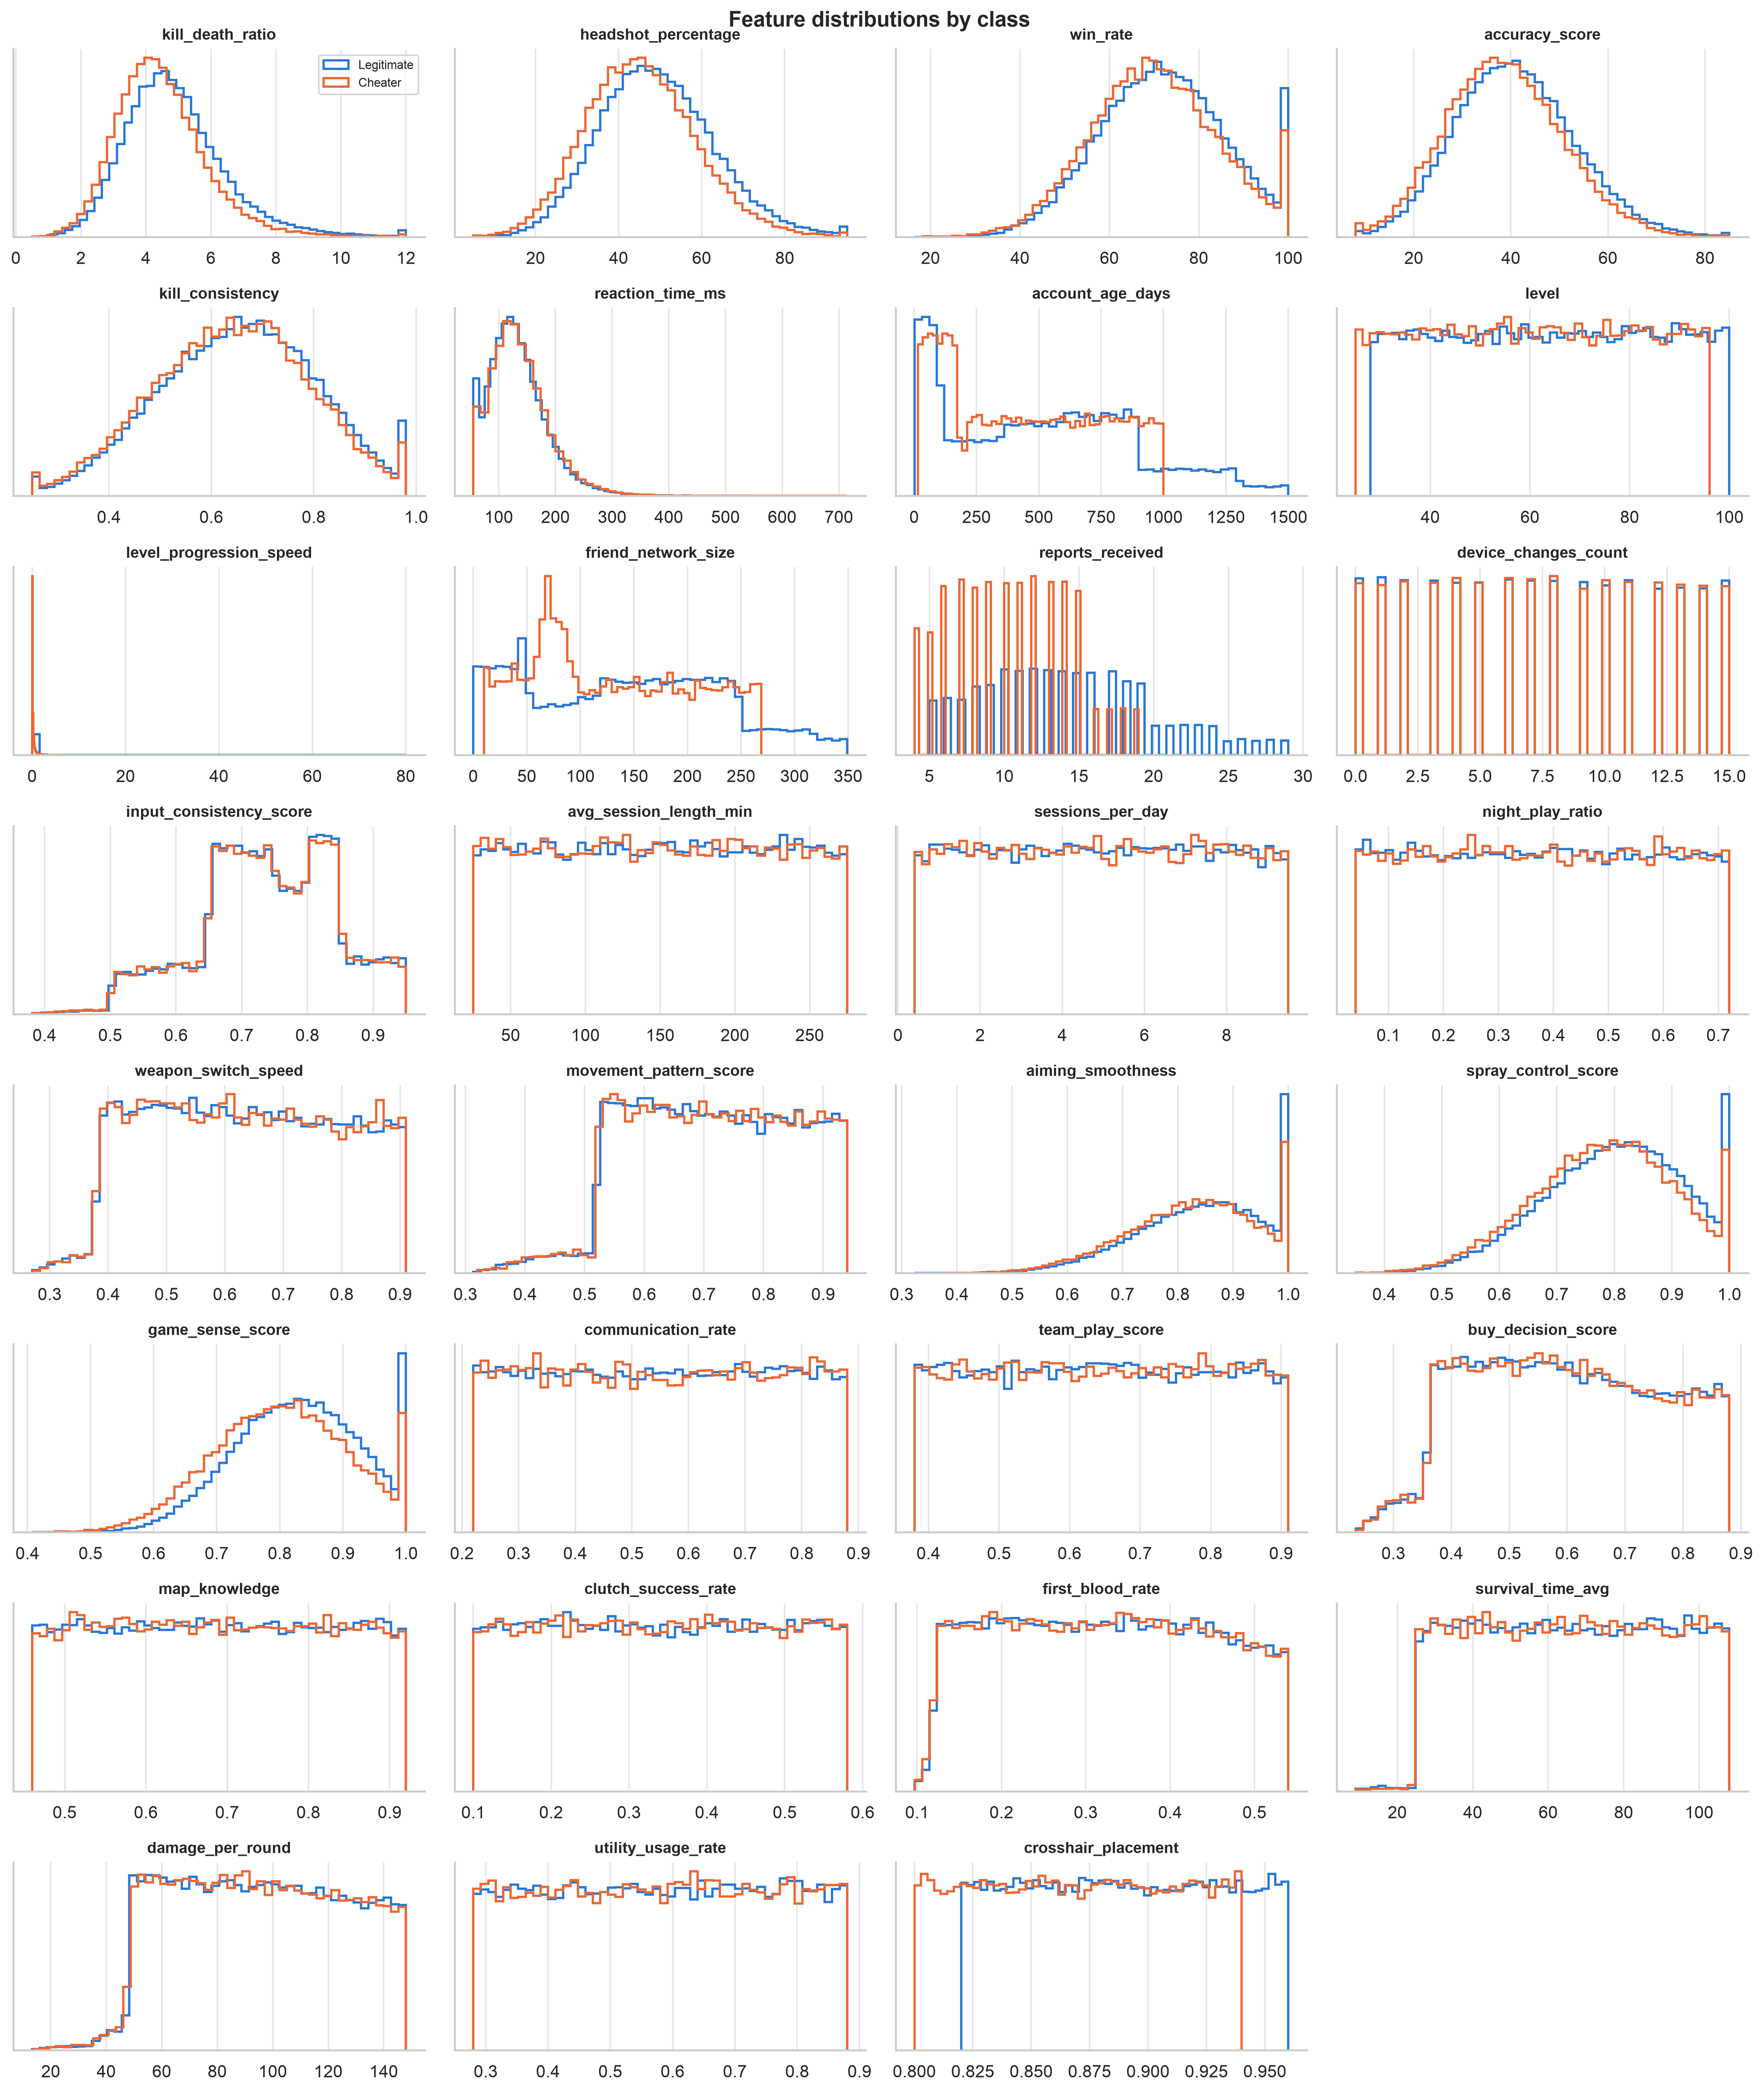
\includegraphics[width=0.92\linewidth]{assets/task1_feature_distributions.png}
\caption{การแจกแจงของฟีเจอร์ทั้ง 31 ตัวแปรใน Task 1 แยกตามกลุ่มสุจริตและผู้โกง แสดงภาวะอั้นที่ขอบบนและขอบเขตช่วงข้อมูลบัญชี}
\label{fig:t1_dist}
\end{figure}

\begin{figure}[H]\centering
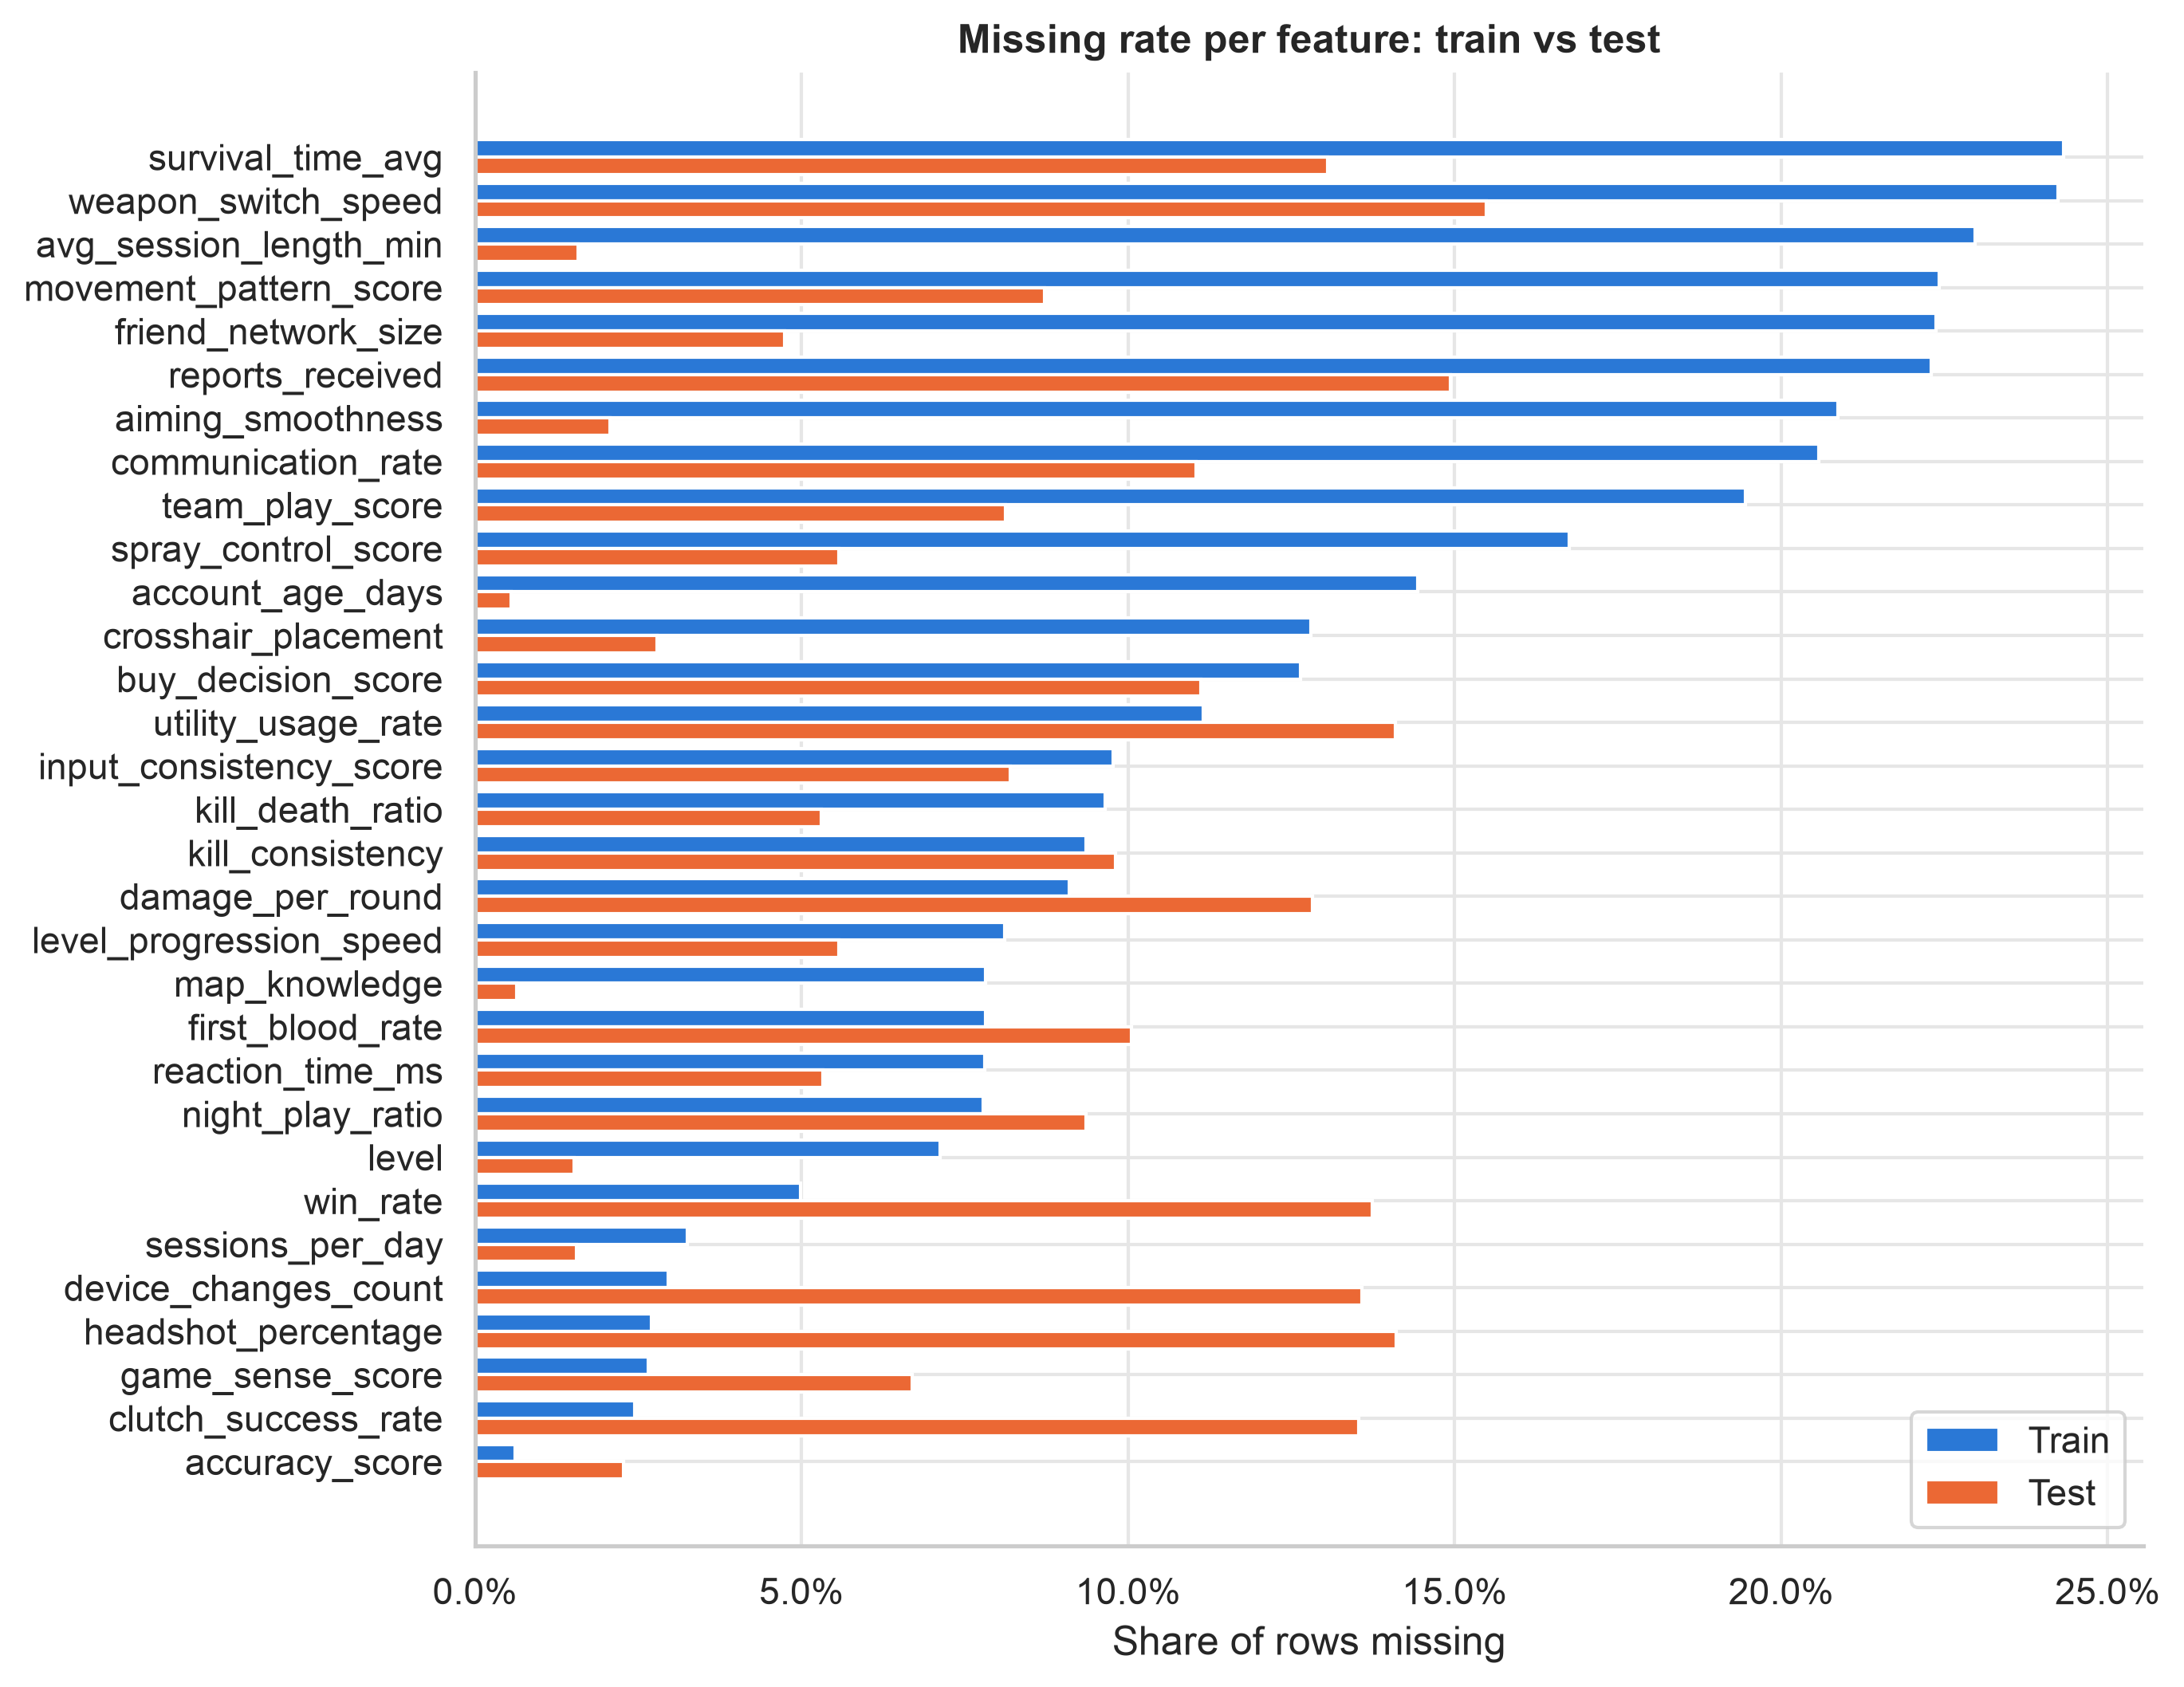
\includegraphics[width=0.86\linewidth]{assets/task1_missing_rate_train_test.png}
\caption{การเปรียบเทียบอัตราข้อมูลขาดหาย (Missing Rate) ระหว่าง Train Set และ Test Set ใน Task 1}
\label{fig:t1_miss}
\end{figure}

\subsection{การเตรียมข้อมูลและการสร้างคุณลักษณะ}
ดำเนินการภายใต้ 5-Fold Stratified K-Fold (\code{SEED=42}) บนข้อมูลที่มีป้ายกำกับ $90{,}816$ แถว โดยสร้างคุณลักษณะ 3 ระดับในทุก Training Fold:
\begin{enumerate}[leftmargin=1.8em,itemsep=2pt]
    \item \textbf{Physical Account Invariants:} เติมค่าอายุบัญชีด้วยสมการเชิงฟิสิกส์ของความก้าวหน้า (\code{age\_filled = 0.615 * level / level\_progression\_speed}) พร้อมสร้างอัตราส่วนเชิงพฤติกรรม \code{friends\_per\_day}, \code{reports\_per\_day}, \code{kd\_x\_acc} และ \code{aim\_comp} พร้อมชุดคัดกรอง 28 ฟีเจอร์หลัก (\code{COLS\_20\_FE}) ควบคู่กับชุด 31 ฟีเจอร์เดิม
    \item \textbf{Fold-Safe Aim-vs-Tactics Z-Gaps:} คำนวณค่ามาตรฐาน Z-score ของกลุ่มตัวชี้วัดทักษะการยิงและยุทธวิธีจำนวน 11 ตัวแปรภายในแต่ละ Training Fold (คงค่า \code{NaN} เดิมไว้ให้ Tree Model จัดการตามธรรมชาติ) แล้วสร้างส่วนต่างความต่างเชิงทักษะ ได้แก่ \code{aim\_minus\_tactics\_z}, \code{hs\_minus\_gs\_z} และ \code{xhair\_minus\_map\_z}
    \item \textbf{Analytical 8-Cohort Support \& 5-Profile Tobit-MVN5:} ถอดแบบจำลองกำเนิดข้อมูลเชิงวิเคราะห์ผ่าน 2 กลไก คือ (ก) โมเดลความน่าจะเป็นของ 8 กลุ่มประชากรบัญชี (4 Clean Cohorts, 4 Cheater Cohorts) โดยอินทิเกรตตัวแปรที่ขาดหายด้วย 12-Point Gauss-Legendre Quadrature และ (ข) แบบจำลอง \textbf{1D Tobit EM} สำหรับ \code{game\_sense\_score} ที่ถูกตัดขอบขวาที่ $1.0$ ร่วมกับ Yeo-Johnson Shrunk-Covariance Multivariate Normal EM ($\text{shrink}=0.3$, 12 รอบ EM) เพื่อจำแนกโปรไฟล์ทักษะ 5 กลุ่ม โดยฝึกกึ่งมีผู้สอนเฉพาะ Training Fold ร่วมกับข้อมูลไม่มีป้ายกำกับ $13{,}184$ แถวในไฟล์ฝึกสอน
\end{enumerate}

\subsection{การออกแบบโมเดลและผลลัพธ์การทดลอง}

โมเดลฐาน Logistic Regression ทำคะแนน OOF ROC-AUC $= 0.76782$ และ Nested $F_2 = 0.76637$ เท่านั้น เมื่อเพิ่มความละเอียด Bin Resolution ของ GBDTs (\code{LightGBM max\_bin=2047}, \code{XGBoost hist max\_bin=4096}, \code{CatBoost border\_count=1024}) ร่วมกับกฎสนับสนุนขอบเขตจากชุดฝึกสอน (\code{HardSupport Clamp}: แยกแถวที่มั่นใจสูงได้ \code{det\_y0 = 25,977} ผิด 1 ราย และ \code{det\_y1 = 9,922} ผิด 0 รายบน OOF) แล้วผสม 5 โมเดลด้วย Nested SLSQP Stack ค่า AUC เพิ่มเป็น $0.89477$ และ $F_2 = 0.83920$

จากนั้นเมื่อนำมาผสานเข้ากับ Analytical Cohort Logistic Regression และ 5-Profile Semi-Supervised Tobit-MVN5 โดยปรับน้ำหนักตามความครบถ้วนของข้อมูล (\code{(0.70, 0.10, 0.20)} สำหรับแถวครบถ้วน และ \code{(0.45, 0.40, 0.15)} สำหรับแถวที่มีค่าขาดหาย) โมเดลขั้นสุดท้ายบรรลุ \textbf{OOF Binary $F_2 = 0.841552$}, \textbf{ROC-AUC $= 0.896762$}, PR-AUC $= 0.840860$ และ LogLoss $= 0.350709$ ณ จุดตัด $\tau^* = 0.199023$ โดยปรับปรุงคะแนนดีขึ้นครบทั้ง 5 Folds เหนือขั้นตอนก่อนหน้า (\code{0.840965}, Paired Bootstrap 95\% CI \code{[+0.000158, +0.001005]}) รายละเอียดทั้งหมดแสดงใน \textbf{ตารางที่~\ref{tab:t1_ablation}}, \textbf{ตารางที่~\ref{tab:t1_folds}} และ \textbf{รูปที่~\ref{fig:t1_diag}}

\begin{table}[H]\centering
{\fontsize{9.5}{12.5}\selectfont\arrayrulecolor{RuleGray}
\caption{เปรียบเทียบผล 5-Fold Out-of-Fold ของแบบจำลองแต่ละขั้นใน Task 1}
\label{tab:t1_ablation}
\begin{tabular}{L{6.8cm}ccccc}
\toprule
\rowcolor{TableHead} \textbf{สถาปัตยกรรม / ขั้นตอนการทดลอง} & \textbf{ROC-AUC} & \textbf{Def $F_2$} & \textbf{Nested $F_2$} & \textbf{LogLoss} & \textbf{$\tau^*$} \\
\midrule
1. Logistic Regression Baseline (Fold-Safe) & 0.76782 & 0.48595 & 0.76637 & 0.53577 & 0.1394 \\
2. Full CleanDGP LGBM + HardSupport Clamp & 0.89448 & 0.63491 & 0.83919 & 0.35504 & 0.1681 \\
3. Interior 4-Model Specialist + HardClamp & 0.89400 & 0.63454 & 0.83888 & 0.35574 & 0.1822 \\
4. Semi-Supervised CleanZ LGBM + HardClamp & 0.89417 & 0.63435 & 0.83920 & 0.35539 & 0.1824 \\
5. Semi-Supervised XGBoost 4096 + HardClamp & 0.89391 & 0.62731 & 0.83907 & 0.35583 & 0.1943 \\
6. Semi-Supervised CatBoost 1024 + HardClamp & 0.89166 & 0.63582 & 0.83793 & 0.35833 & 0.1533 \\
7. 5-Stream Pure-Train Nested SLSQP Stack & 0.89477 & 0.63342 & 0.83920 & 0.35466 & 0.1750 \\
8. Analytical Cohort Support + GBDT Hybrid & 0.89526 & 0.63240 & 0.84043 & 0.35257 & 0.1829 \\
9. Cohort LR Account Likelihood Blend & 0.89646 & 0.63199 & 0.84097 & 0.35110 & 0.1935 \\
10. Semi-Sup 5-Profile Tobit-MVN (Standalone) & 0.89664 & 0.63497 & 0.84058 & 0.35052 & 0.1834 \\
\rowcolor{TableHead} \textbf{11. Cohort LR + Tobit-MVN5 Hybrid (Final)} & \textbf{0.89676} & \textbf{0.63281} & \textbf{0.84155} & \textbf{0.35071} & \textbf{0.1990} \\
\bottomrule
\end{tabular}}
\end{table}

\begin{table}[H]\centering
{\fontsize{9.5}{12.5}\selectfont\arrayrulecolor{RuleGray}
\caption{คะแนน $F_2$ ราย Fold ของระบบ Hybrid ขั้นสุดท้ายใน Task 1 (ชนะครบทั้ง 5 Folds)}
\label{tab:t1_folds}
\begin{tabular}{cccccc}
\toprule
\rowcolor{TableHead} \textbf{Fold} & \textbf{Cohort + GBDT $F_2$} & \textbf{Cohort LR Blend $F_2$} & \textbf{Final Hybrid $F_2$} & \textbf{$\Delta$ Gain} & \textbf{Threshold $\tau^*$} \\
\midrule
0 & 0.839041 & 0.839418 & 0.840027 & +0.000609 & 0.199023 \\
1 & 0.841513 & 0.841330 & 0.841807 & +0.000477 & 0.199057 \\
2 & 0.841050 & 0.842079 & 0.842689 & +0.000610 & 0.199023 \\
3 & 0.838370 & 0.839360 & 0.839489 & +0.000128 & 0.199023 \\
4 & 0.842151 & 0.842642 & 0.843752 & +0.001110 & 0.199023 \\
\bottomrule
\end{tabular}}
\end{table}

\begin{figure}[H]\centering
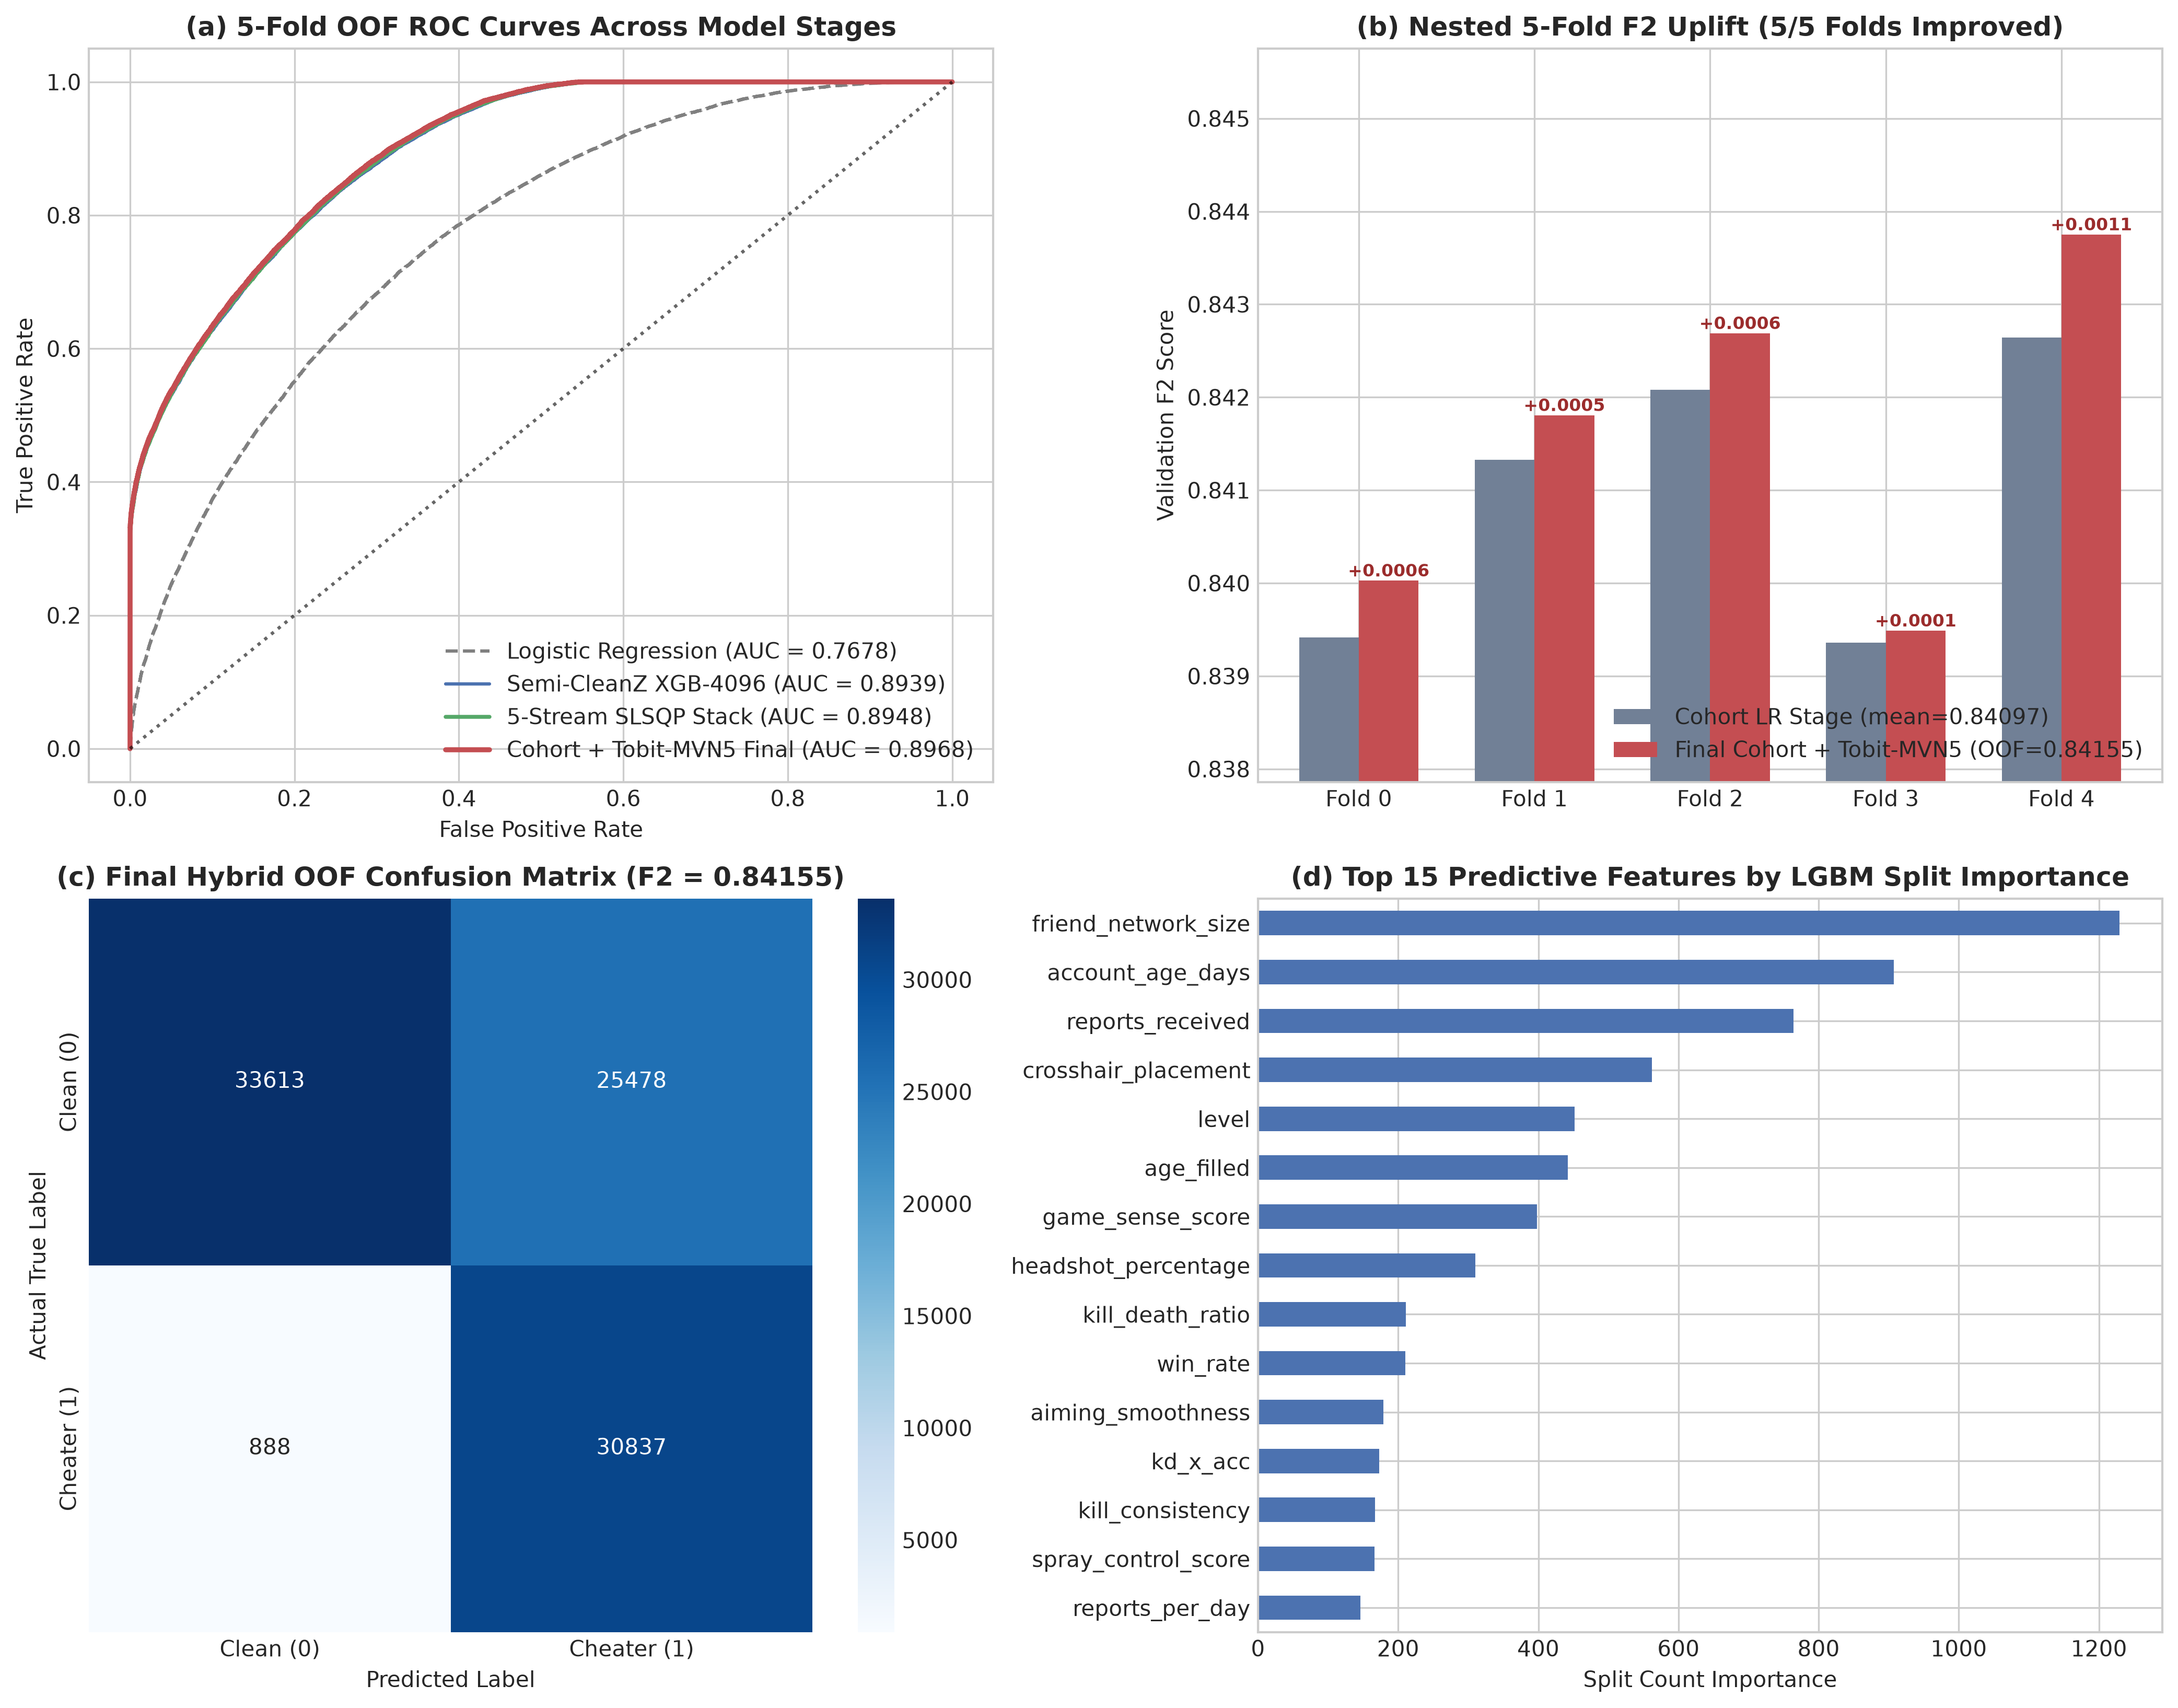
\includegraphics[width=0.95\linewidth]{assets/task1_diagnostics.png}
\caption{การวิเคราะห์ผลของ Task 1: เส้นโค้ง ROC ข้ามขั้นตอน การยกระดับ $F_2$ ทั้ง 5 Folds เมทริกซ์ความสับสน OOF และตัวแปรสำคัญ 15 อันดับแรกจาก LightGBM}
\label{fig:t1_diag}
\end{figure}

\begin{figure}[H]\centering
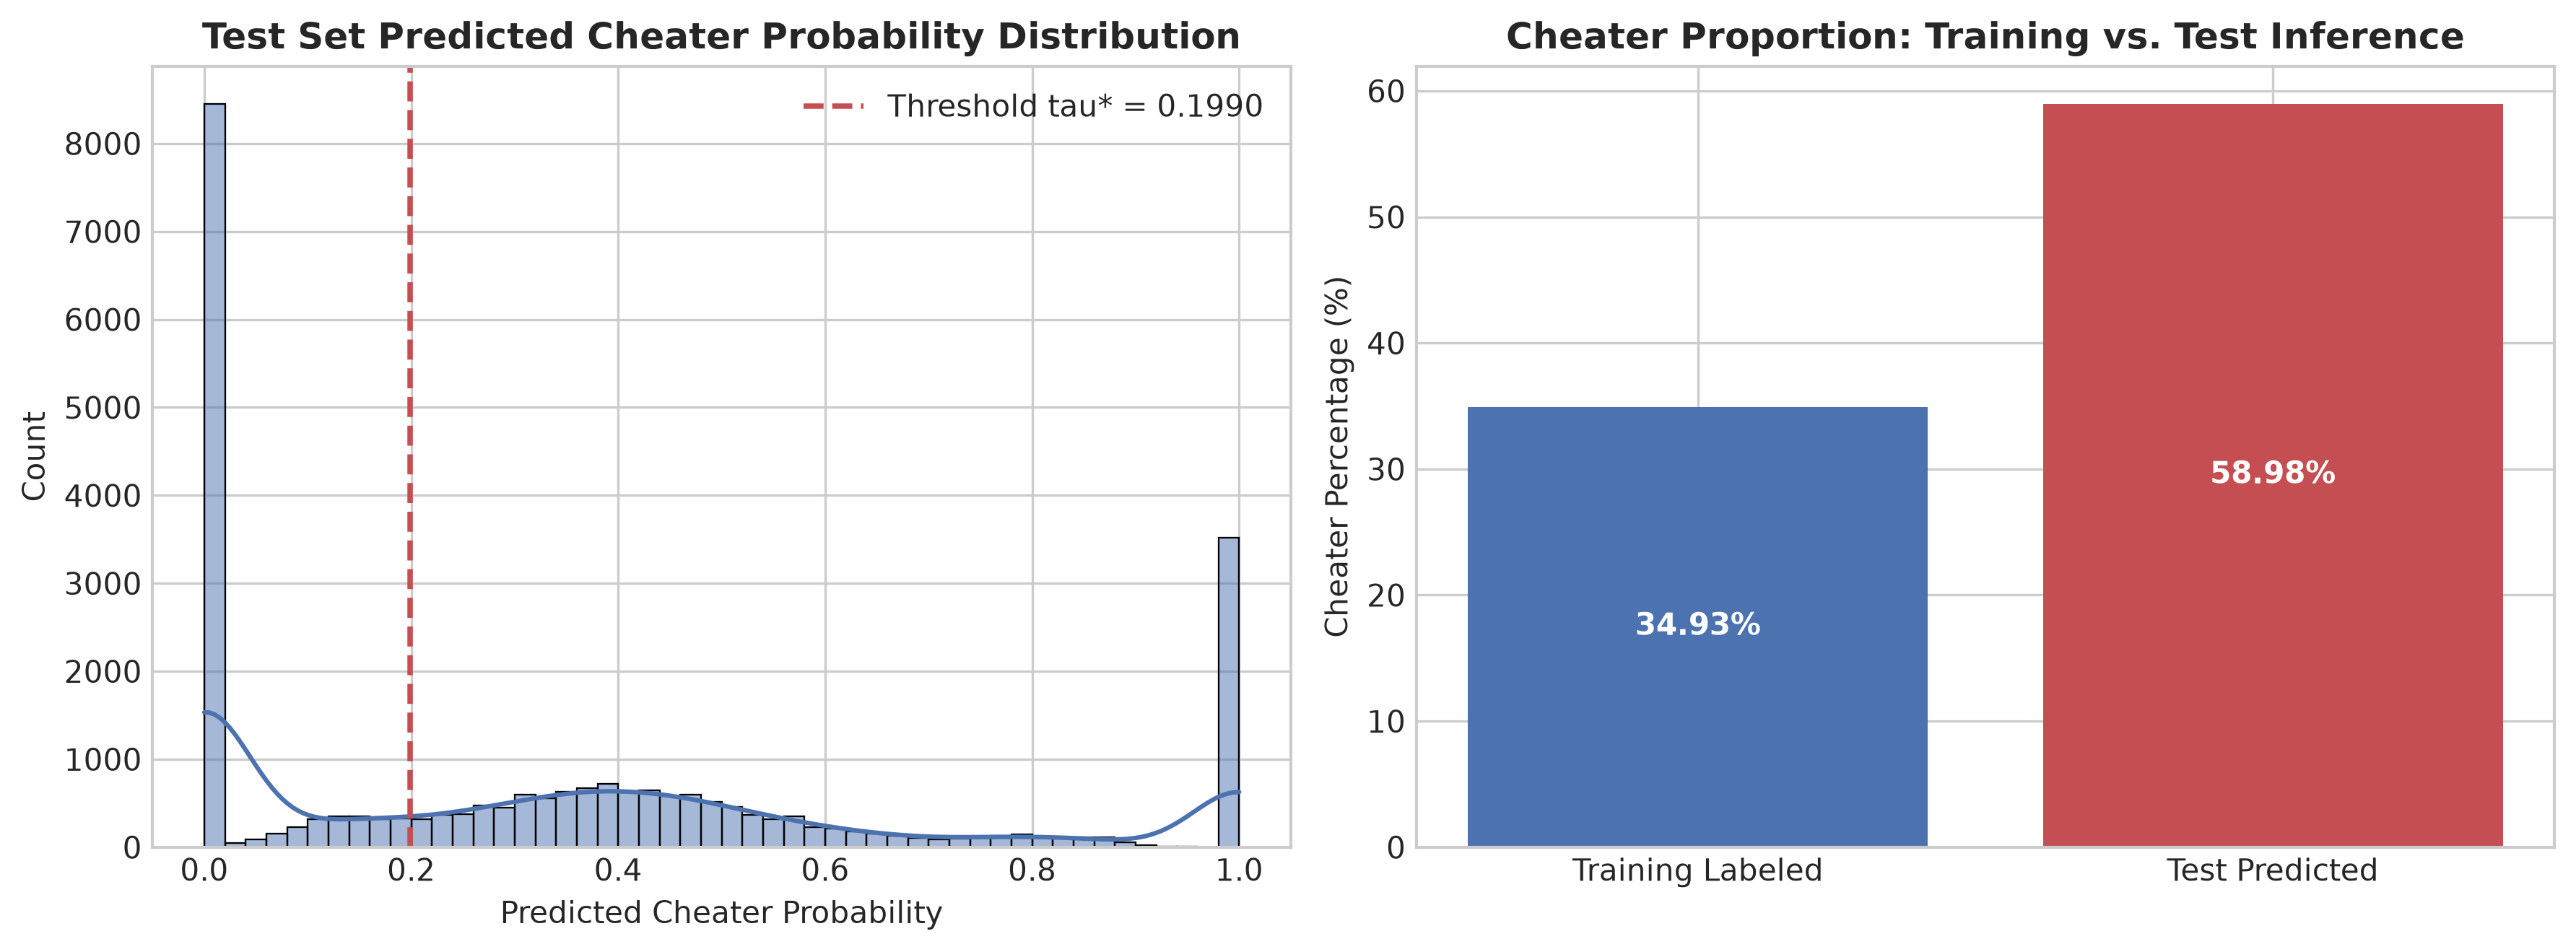
\includegraphics[width=0.88\linewidth]{assets/task1_test_alignment.png}
\caption{การกระจายตัวของความน่าจะเป็นบน Test Set เทียบจุดตัด $\tau^* = 0.1990$ และสัดส่วนการตรวจพบบัญชีโกง (15,270 จาก 25,889 บัญชี = 58.98\%)}
\label{fig:t1_align}
\end{figure}

\subsection{การวิเคราะห์ข้อผิดพลาดและการตีความเชิงธุรกิจ}

ปัญหาสำคัญที่พบในช่วงทดลองแรกคือโมเดลที่ใช้เพียง Tree Ensemble 15 ฟีเจอร์ทำผลงานตกต่ำบนข้อมูลที่มีค่าขาดหายและข้อมูลที่ถูกตัดขอบขวา (\code{game\_sense\_score = 1.0}) การเสริมสมการ Tobit Likelihood และการแยกน้ำหนักระหว่างแถวที่ข้อมูลครบถ้วนกับข้อมูลขาดหายช่วยยกระดับ $F_2$ ของกลุ่มข้อมูลขาดหายจาก $0.82599$ ขึ้นมาเป็น $0.82776$ (ส่วนกลุ่มข้อมูลครบถ้วนได้ $0.86137$)

ในมิติการปฏิบัติงานจริง (\textbf{รูปที่~\ref{fig:t1_align}}) แม้ตัวแบบจะติดธงผู้ต้องสงสัย $15{,}270 / 25{,}889$ บัญชี ($58.98\%$) เพื่อรักษาค่า Recall ตามวัตถุประสงค์ $F_2$ แต่สามารถคัดกรองบัญชีสุจริตบนขอบเขตแน่นอนออกได้ $8{,}266$ บัญชี ($31.93\%$) โดยไม่สร้างการแบนผิดพลาด และดึงกลุ่มโกงแน่นอน $3{,}341$ บัญชี ($12.91\%$) เข้าสู่คิวระงับเร่งด่วน ทำให้ทีมตรวจสอบที่มีขีดจำกัด 500 คดีต่อวันทำงานได้อย่างตรงจุดและลดปัญหาผู้เล่นสุจริตออกจากระบบ

% ==============================================================================
\clearpage
\section{Task 2: Player Segment Classification (Multi-Class Classification)}

\subsection{คำอธิบายปัญหาและการสำรวจข้อมูลเบื้องต้น}
Task 2 จัดกลุ่มผู้เล่นออกเป็น 4 กลุ่มพฤติกรรม ได้แก่ \code{0=Casual} ($40{,}957$ ราย หรือ $39.38\%$), \code{1=Core/Grinder} ($26{,}032$ ราย หรือ $25.03\%$), \code{2=Social/Hardcore} ($21{,}029$ ราย หรือ $20.22\%$) และ \code{3=Whale} ($15{,}982$ ราย หรือ $15.37\%$) จากข้อมูลฝึกสอน $104{,}000 \times 46$ คอลัมน์ และชุดทดสอบ $25{,}889 \times 45$ คอลัมน์ ภายใต้มาตรวัด \textbf{Unweighted Macro $F_1$} เนื่องจากคลาส 0 มีจำนวนมากกว่าคลาส 3 ถึง $2.56$ เท่า การทำนายด้วยค่า \code{argmax} ปกติจึงกดทอนการทำนายกลุ่ม Whale และ Hardcore นอกจากนี้ ชุดข้อมูลยังแทรกฟีเจอร์สัญญาณรบกวนชัดเจน 3 คอลัมน์ (\code{random\_metric\_1..3}) ซึ่งจำเป็นต้องคัดออกก่อนฝึกสอน

\subsection{การเตรียมข้อมูลและการออกแบบคุณลักษณะ}
หลังจากตัดคอลัมน์รหัสและสัญญาณรบกวน \code{random\_metric\_1..3} ออกทั้งหมด คณะผู้จัดทำแปลงตัวแปรลำดับ (\code{ENG\_MAP: Low=1..Veteran=4}, \code{LOY\_MAP: Bronze=1..Diamond=5}) จนได้ชุดคุณลักษณะสะอาด \code{Clean28} (25 ตัวแปรเชิงปริมาณและ 3 ตัวแปรอันดับ) แล้วสร้างฟีเจอร์เสริมภายในแต่ละ Fold ของ 5-Fold Stratified K-Fold (\code{SEED=42}) ดังนี้
\begin{enumerate}[leftmargin=1.8em,itemsep=2pt]
    \item \textbf{Missing-Aware ZLR Probabilities (\code{Clean28+ZLR}):} มาตรฐานข้อมูล Z-score ร่วมกับตัวแปรบ่งชี้ค่าว่างผ่าน Multinomial Logistic Regression ภายใน Fold เพื่อผลิตความน่าจะเป็นฐาน \code{lr\_p0..lr\_p3}
    \item \textbf{Orthogonal Persona-Axis Z-Scores (56 คอลัมน์):} สังเคราะห์ค่าเฉลี่ยและส่วนเบี่ยงเบนตาม 4 แกนพฤติกรรมหลัก (Spend, Engagement, Social, Competitive) พร้อมความต่างข้ามแกน (เช่น \code{spend\_minus\_engage\_z}, \code{spend\_minus\_comp\_z}) และอัตราส่วนเชิงประสิทธิภาพต่อเวลาเล่น (\code{spend\_per\_hour}, \code{spend\_per\_freq})
\end{enumerate}

\subsection{การพัฒนาแบบจำลองและการปรับเทียบ Affine Bayes Decision Rule}

คณะผู้จัดทำประเมินโมเดลฐาน 7 ตระกูลบน 5-Fold SKF ได้แก่ Parametric Expectation-Maximization Density (\code{ExactParamEM}, OOF LogLoss $= 0.59563$), \code{XGB\_Clean28}, \code{LGB\_Clean28}, \code{CB\_Clean28} (CatBoost), Deep Tabular \code{CleanTabM\_SWA3}, \code{Fact\_Clean28} และ \code{Oven\_Rev} พบว่า \code{ExactParamEM} จับโครงสร้างประชากรได้ดีที่สุด และเมื่อผสานความน่าจะเป็นในสัดส่วน \textbf{0.90 ExactParamEM + 0.10 CB\_Clean28} ช่วยเสริมความแม่นยำบริเวณเส้นแบ่งระหว่างกลุ่ม (Decision Boundary, $\text{margin} < 0.02$)

หลังจากนั้นจึงปรับเทียบความน่าจะเป็นด้วย 4-Parameter Zero-Mean Logit Bias (\code{bias = [+0.002124, +0.002960, -0.006227, +0.001143]}) และประยุกต์ใช้กฎตัดสินใจที่เหมาะสมที่สุดสำหรับ Macro-$F_1$ ในรูป \textbf{Affine Bayes Fixed-Point Rule}:
$$\hat{y}_i = \arg\max_{c \in \{0,1,2,3\}} \bigl(\alpha_c p_{i,c} - \beta_c\bigr)$$
โดย $\alpha = [2.4982, 3.9719, 5.0147, 6.7329]$ และ $\beta = [1.0252, 1.4845, 1.8033, 2.5184]$ ผลลัพธ์จาก Cross-Fitted Validation บรรลุ \textbf{Macro-$F_1 = 0.759799$} (Accuracy $77.21\%$, LogLoss $0.595756$) ชนะ \code{ExactParamEM} เดี่ยว ($0.759201$) ครบทั้ง 5 Folds ($0.75806$, $0.75766$, $0.76186$, $0.75902$, $0.76236$) รายละเอียดแสดงใน \textbf{ตารางที่~\ref{tab:t2_ablation}}, \textbf{ตารางที่~\ref{tab:t2_perclass}} และ \textbf{รูปที่~\ref{fig:t2_diag}}

\begin{table}[H]\centering
{\fontsize{9.5}{12.5}\selectfont\arrayrulecolor{RuleGray}
\caption{เปรียบเทียบผล 5-Fold Out-of-Fold ของโมเดลทั้ง 7 ตระกูลและขั้นตอนปรับเทียบใน Task 2}
\label{tab:t2_ablation}
\begin{tabular}{L{8.0cm}ccc}
\toprule
\rowcolor{TableHead} \textbf{โมเดล / ขั้นตอนการผสาน} & \textbf{OOF LogLoss} & \textbf{OOF Macro-$F_1$} & \textbf{น้ำหนักผสาน} \\
\midrule
ExactParamEM (Parametric EM Density) & \textbf{0.59563} & 0.75848 (Argmax) & 0.90 \\
XGB\_Clean28 & 0.60190 & 0.75747 & 0.00 \\
LGB\_Clean28 & 0.60208 & 0.75690 & 0.00 \\
CB\_Clean28 & 0.60233 & 0.75705 & 0.10 \\
CleanTabM\_SWA3 & 0.60376 & 0.75589 & 0.00 \\
Fact\_Clean28 & 0.61358 & 0.75571 & 0.00 \\
Oven\_Rev & 0.61651 & 0.75131 & 0.00 \\
Cross-Fitted 7-Model Blend (Raw Argmax) & 0.59576 & 0.75867 & --- \\
ExactParamEM (Cross-Fitted Affine Macro-$F_1$ Rule) & 0.59563 & 0.75920 & 1.00 \\
\rowcolor{TableHead} \textbf{0.90 ExactParamEM + 0.10 CB\_Clean28 + Logit-Bias + Affine Rule} & 0.59576 & \textbf{0.75980} & \textbf{Final} \\
\bottomrule
\end{tabular}}
\end{table}

\begin{table}[H]\centering
{\fontsize{9.5}{12.5}\selectfont\arrayrulecolor{RuleGray}
\caption{ประสิทธิภาพรายกลุ่มผู้เล่นของโมเดลขั้นสุดท้าย Task 2 (OOF 104,000 แถว) และสัดส่วนบน Test Set}
\label{tab:t2_perclass}
\begin{tabular}{lccccc}
\toprule
\rowcolor{TableHead} \textbf{กลุ่มผู้เล่น (Segment)} & \textbf{Support} & \textbf{Precision} & \textbf{Recall} & \textbf{$F_1$-Score} & \textbf{Test Predicted} \\
\midrule
0: Casual Player & 40,957 & 0.8082 & 0.8347 & 0.8212 & 10,587 (40.89\%) \\
1: Core / Grinder & 26,032 & 0.7452 & 0.7540 & 0.7496 & 6,582 (25.42\%) \\
2: Social / Hardcore & 21,029 & 0.7286 & 0.7087 & 0.7185 & 5,012 (19.36\%) \\
3: Whale (Big Spender) & 15,982 & 0.7769 & 0.7246 & 0.7498 & 3,708 (14.32\%) \\
\rowcolor{TableHead} \textbf{Macro Avg / Weighted Avg} & \textbf{104,000} & \textbf{0.7647} & \textbf{0.7555} & \textbf{0.7598} & \textbf{25,889 (100.00\%)} \\
\bottomrule
\end{tabular}}
\end{table}

\begin{figure}[H]\centering
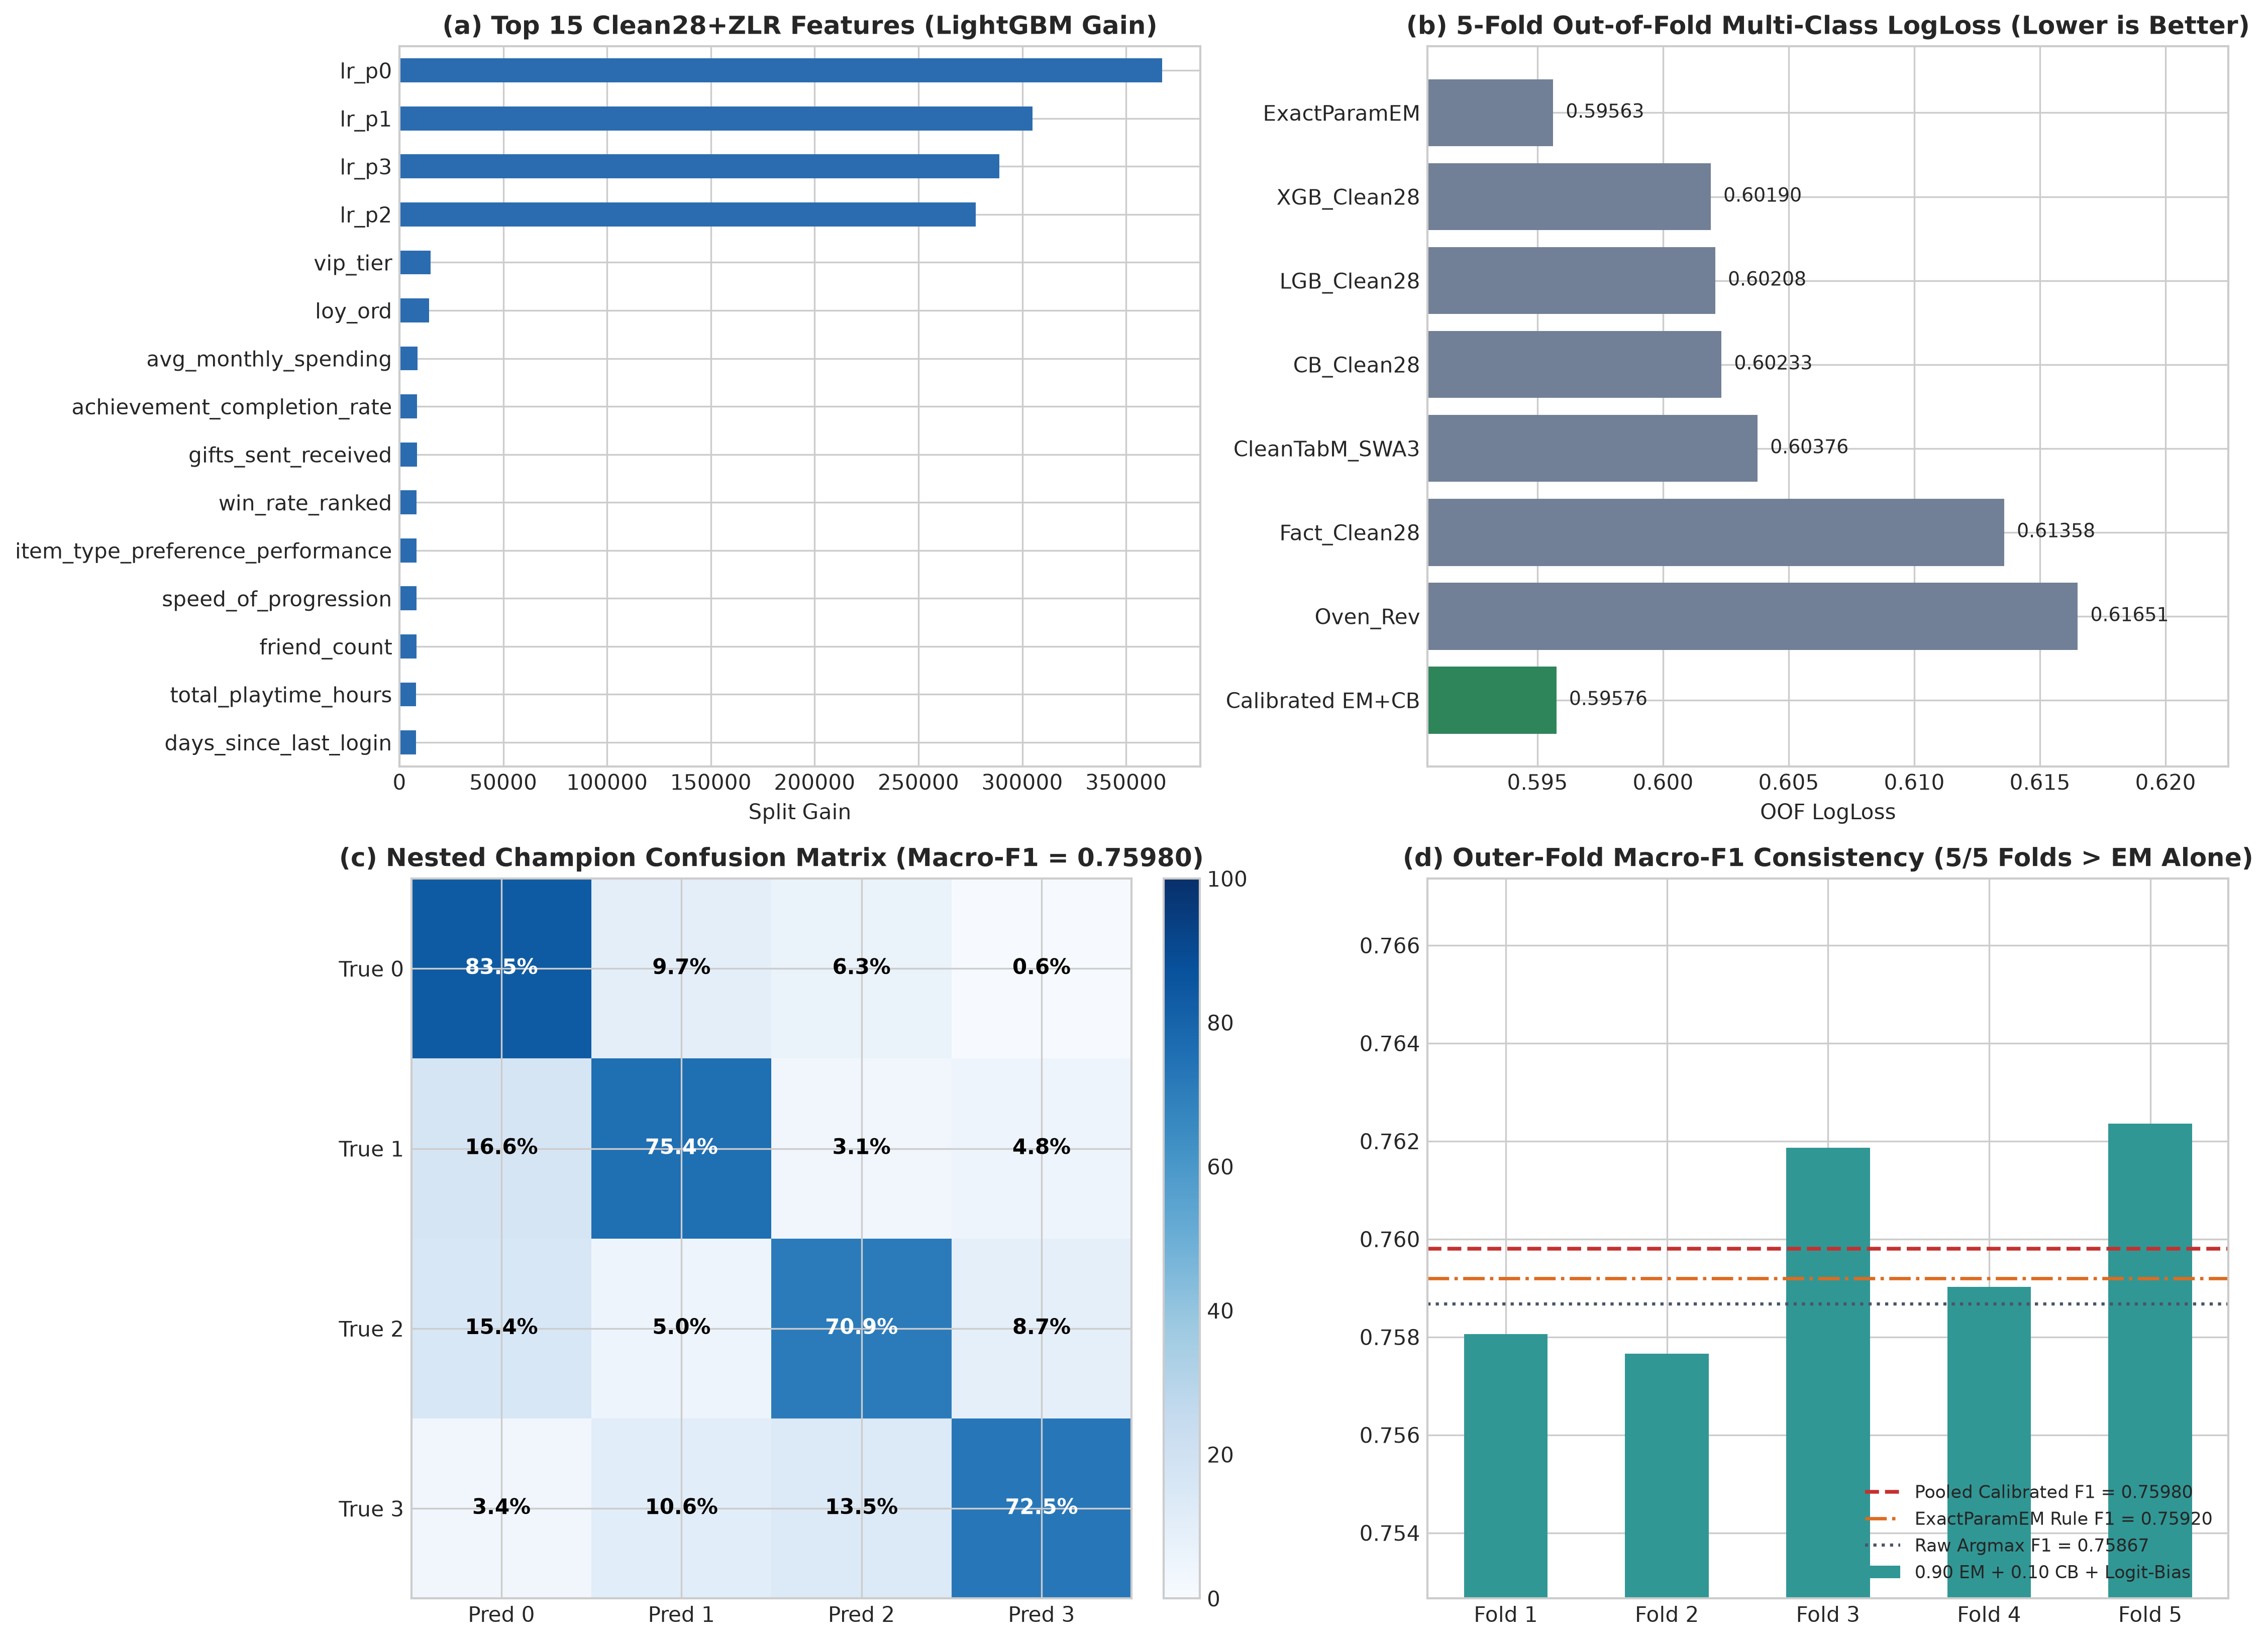
\includegraphics[width=0.95\linewidth]{assets/task2_diagnostics.png}
\caption{การวิเคราะห์ผลของ Task 2: ฟีเจอร์สำคัญของ Clean28+ZLR ค่า OOF LogLoss ของโมเดลทั้ง 7 ตระกูล เมทริกซ์ความสับสน และเสถียรภาพราย Fold}
\label{fig:t2_diag}
\end{figure}

\begin{figure}[H]\centering
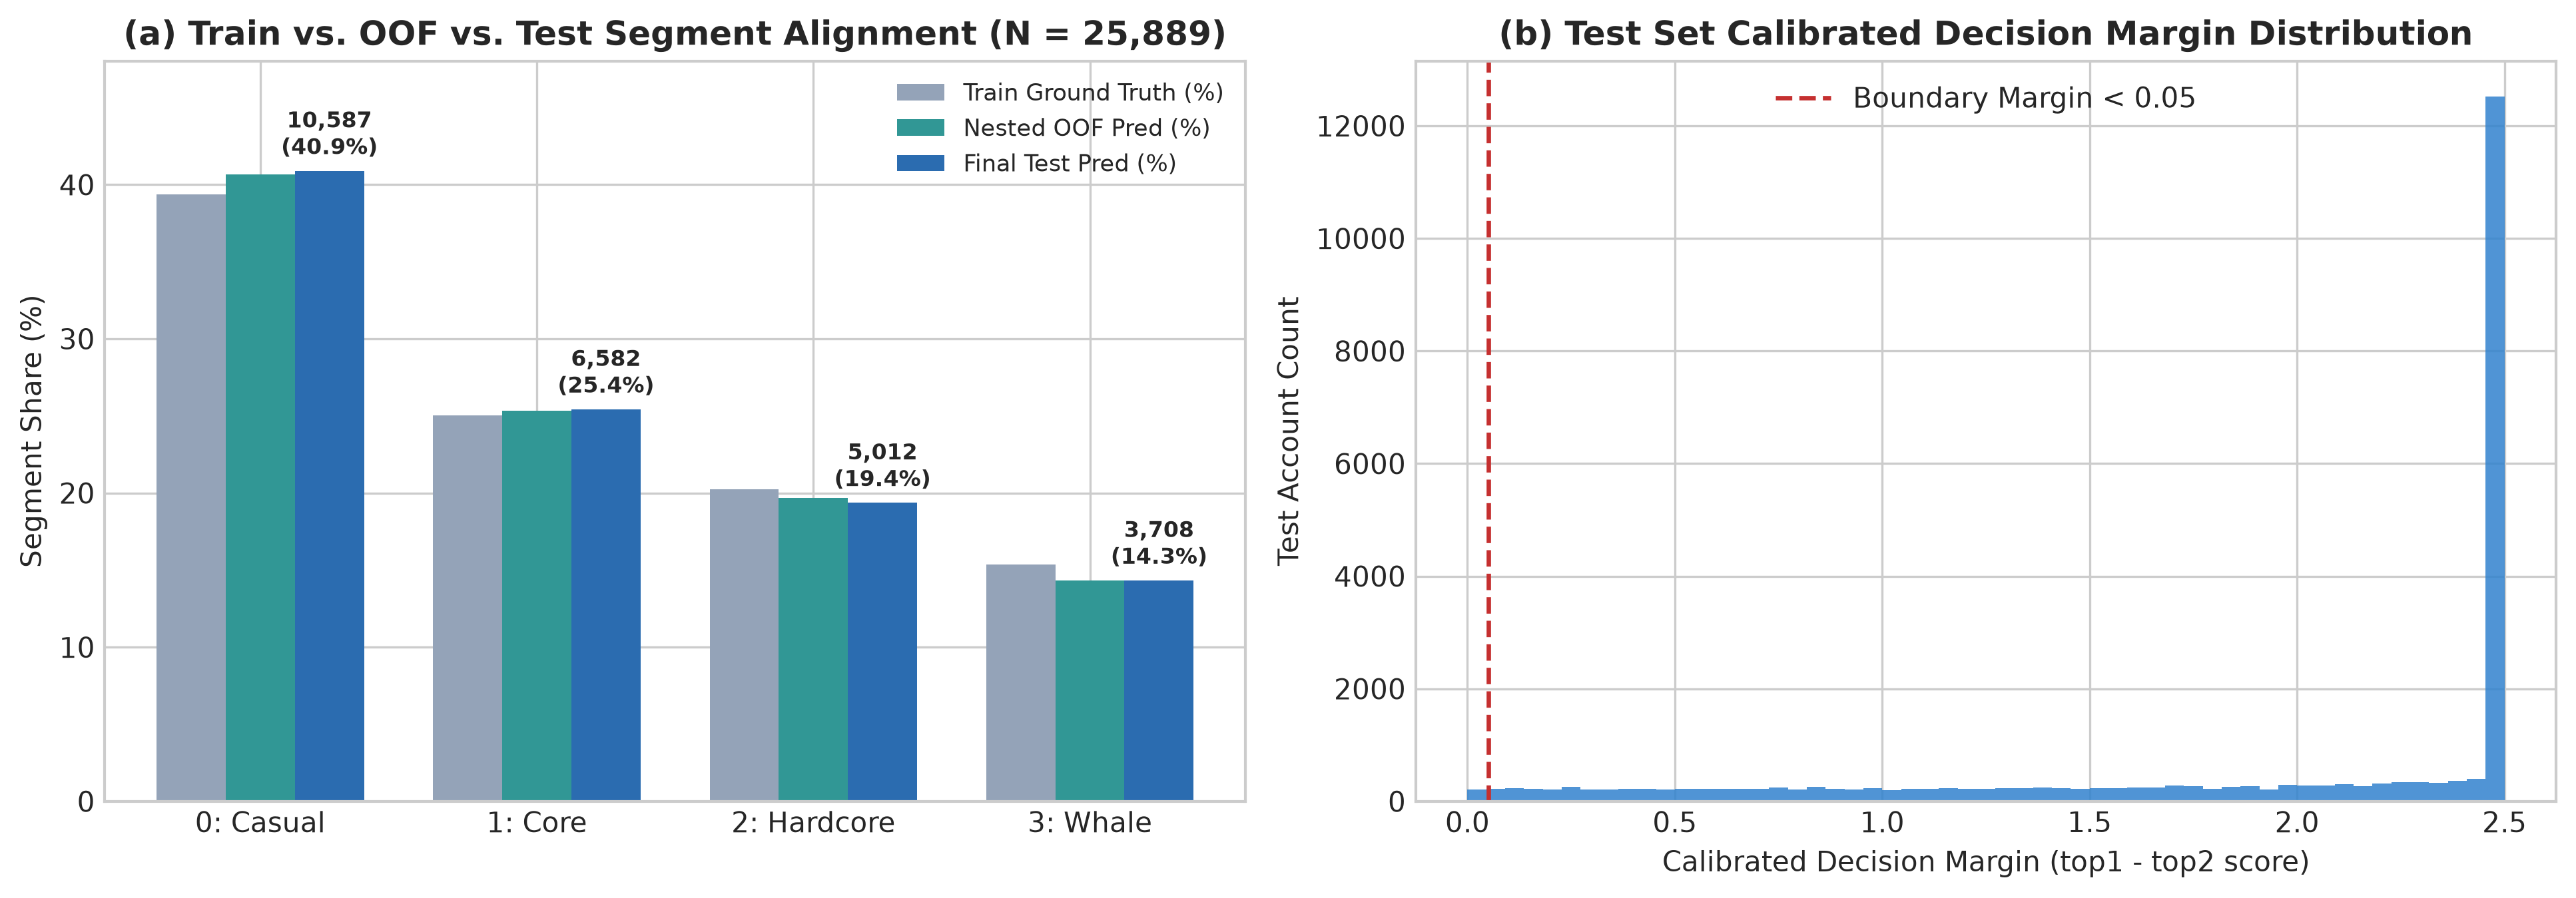
\includegraphics[width=0.88\linewidth]{assets/task2_test_alignment.png}
\caption{ความสอดคล้องของสัดส่วนกลุ่มผู้เล่นระหว่าง Train, OOF และ Test Set (25,889 แถว) พร้อม\mbox{การกระจายตัว}ของ Decision Margin}
\label{fig:t2_align}
\end{figure}

\subsection{ความผิดพลาดที่ค้นพบและผลกระทบต่อธุรกิจ}

ข้อผิดพลาดสำคัญที่พบระหว่างการพัฒนาเกิดขึ้นเมื่อโค้ดขั้นตอน Export ทำนายตกหล่นพจน์ชดเชย $-\beta_c$ ในสมการ $\arg\max_c(\alpha_c p_c - \beta_c)$ ขณะที่การใช้ SLSQP ลด LogLoss แบบรวมศูนย์ตัดน้ำหนัก CatBoost เหลือศูนย์ใน 3 Folds ส่งผลให้ Macro-$F_1$ ลดลงเหลือ $0.753158$ (ทำนายผิดเพี้ยน $1{,}622$ แถว) เมื่อปรับแก้ให้ใช้ฟังก์ชัน \code{predict\_segments} ชุดเดียวกันทั้งใน Validation และ Export พร้อมบังคับใช้น้ำหนัก $0.90/0.10$ และ Cross-Fitted Logit-Bias คะแนนเพิ่มขึ้นอย่างมีนัยสำคัญสู่ \textbf{0.759799} (95\% Paired Bootstrap CI เท่ากับ \code{[+0.000159, +0.000805]}) ทั้งนี้ควรระบุเป็นข้อสังเกตเชิงวิธีวิทยาว่าการจูน Logit Bias และกฎ Affine ดำเนินการแบบ Cross-Fitted บน OOF Probabilities ของโมเดลฐานที่แช่แข็งไว้ (Frozen OOF)

ในเชิงธุรกิจ (\textbf{รูปที่~\ref{fig:t2_align}}) โมเดลสามารถระบุกลุ่ม Whale ได้ถึง $3{,}708$ บัญชี ($14.32\%$) และกลุ่ม Social/Hardcore $5{,}012$ บัญชี ($19.36\%$) ด้วยสัดส่วนที่สอดคล้องกับประชากรจริง ช่วยให้ฝ่ายการตลาดหยุดยิงโปรโมชันราคาถูกให้ผู้เล่นที่พร้อมจ่ายอยู่แล้วและจัดสรรงบ 60 ล้านบาทต่อเดือนได้ตรงกลุ่มเป้าหมาย

% ==============================================================================
\clearpage
\section{Task 3: Monthly Spending Prediction (Regression)}

\subsection{คำอธิบายปัญหา กฎ Bayes-$L_1$ และการสำรวจข้อมูล}
Task 3 มุ่งพยากรณ์ยอดการใช้จ่ายล่วงหน้า 30 วัน (\code{spending\_30d} หน่วยบาท ในช่วง $[0, 300{,}000]$) ภายใต้มาตรวัด \textbf{NMAE Score} จากข้อมูลฝึกสอน $104{,}000 \times 34$ คอลัมน์ (มีค่าว่างรวม $193{,}731$ ช่อง) และชุดทดสอบ $25{,}889 \times 33$ คอลัมน์ (ค่าว่างรวม $48{,}266$ ช่อง) จาก EDA (\textbf{รูปที่~\ref{fig:t3_eda}}) พบเหตุผล 2 ประการที่ทำให้การทำ Regression มาตรฐานไม่ประสบความสำเร็จ

\begin{enumerate}[leftmargin=1.8em,itemsep=2pt]
    \item \textbf{ภาวะ Zero-Inflation 48.12\%:} ผู้เล่น $50{,}049$ รายไม่ใช้จ่ายเลย ($0.00$ บาท) การใช้ตัวพยากรณ์แบบคาดหมาย $E[Y \mid X] = p \cdot E[Y \mid Y>0, X]$ จะทายเลขบวกเล็กน้อยให้คนกลุ่มนี้เกือบทั้งหมด ทำให้ผลรวม $|y_i - \hat{y}_i|$ สูงเกินความจำเป็น
    \item \textbf{ภาวะ Heavy Right Tail และ Whale Spike:} ในกลุ่มผู้จ่ายเงิน $53{,}951$ ราย ($51.88\%$) ยอดเงินกระจายตัวกว้าง 5 อันดับขนาด ตั้งแต่ $0.09$ บาท, มัธยฐาน $2{,}314.05$ บาท, ค่าเฉลี่ย $20{,}234.88$ บาท, เปอร์เซ็นไทล์ที่ 99 เท่ากับ $184{,}398.64$ บาท จนถึงเพดาน $300{,}000.00$ บาท โดยมีองค์ประกอบการสุ่มจ่ายก้อนใหญ่ $\text{Uniform}[50{,}000, 300{,}000]$ ปะปนในกลุ่ม Segment 3 (Whale)
\end{enumerate}

ภายใต้การลดผลรวม $|y_i - \hat{y}_i|$ (สมมูลกับการเพิ่ม NMAE Score) คำตอบ Bayes-$L_1$ Optimal Forecast ที่แท้จริงเมื่อทราบ $p_i = P(Y_i > 0 \mid X_i)$ คือ:
$$\hat{y}_i^* = \begin{cases} 0 & \text{ถ้า } p_i \le 0.5 \\ Q_{q^*(p_i)}(Y_i \mid Y_i > 0, X_i), \quad q^*(p_i) = 1 - \dfrac{1}{2 p_i} & \text{ถ้า } p_i > 0.5 \end{cases}$$

\begin{figure}[H]\centering
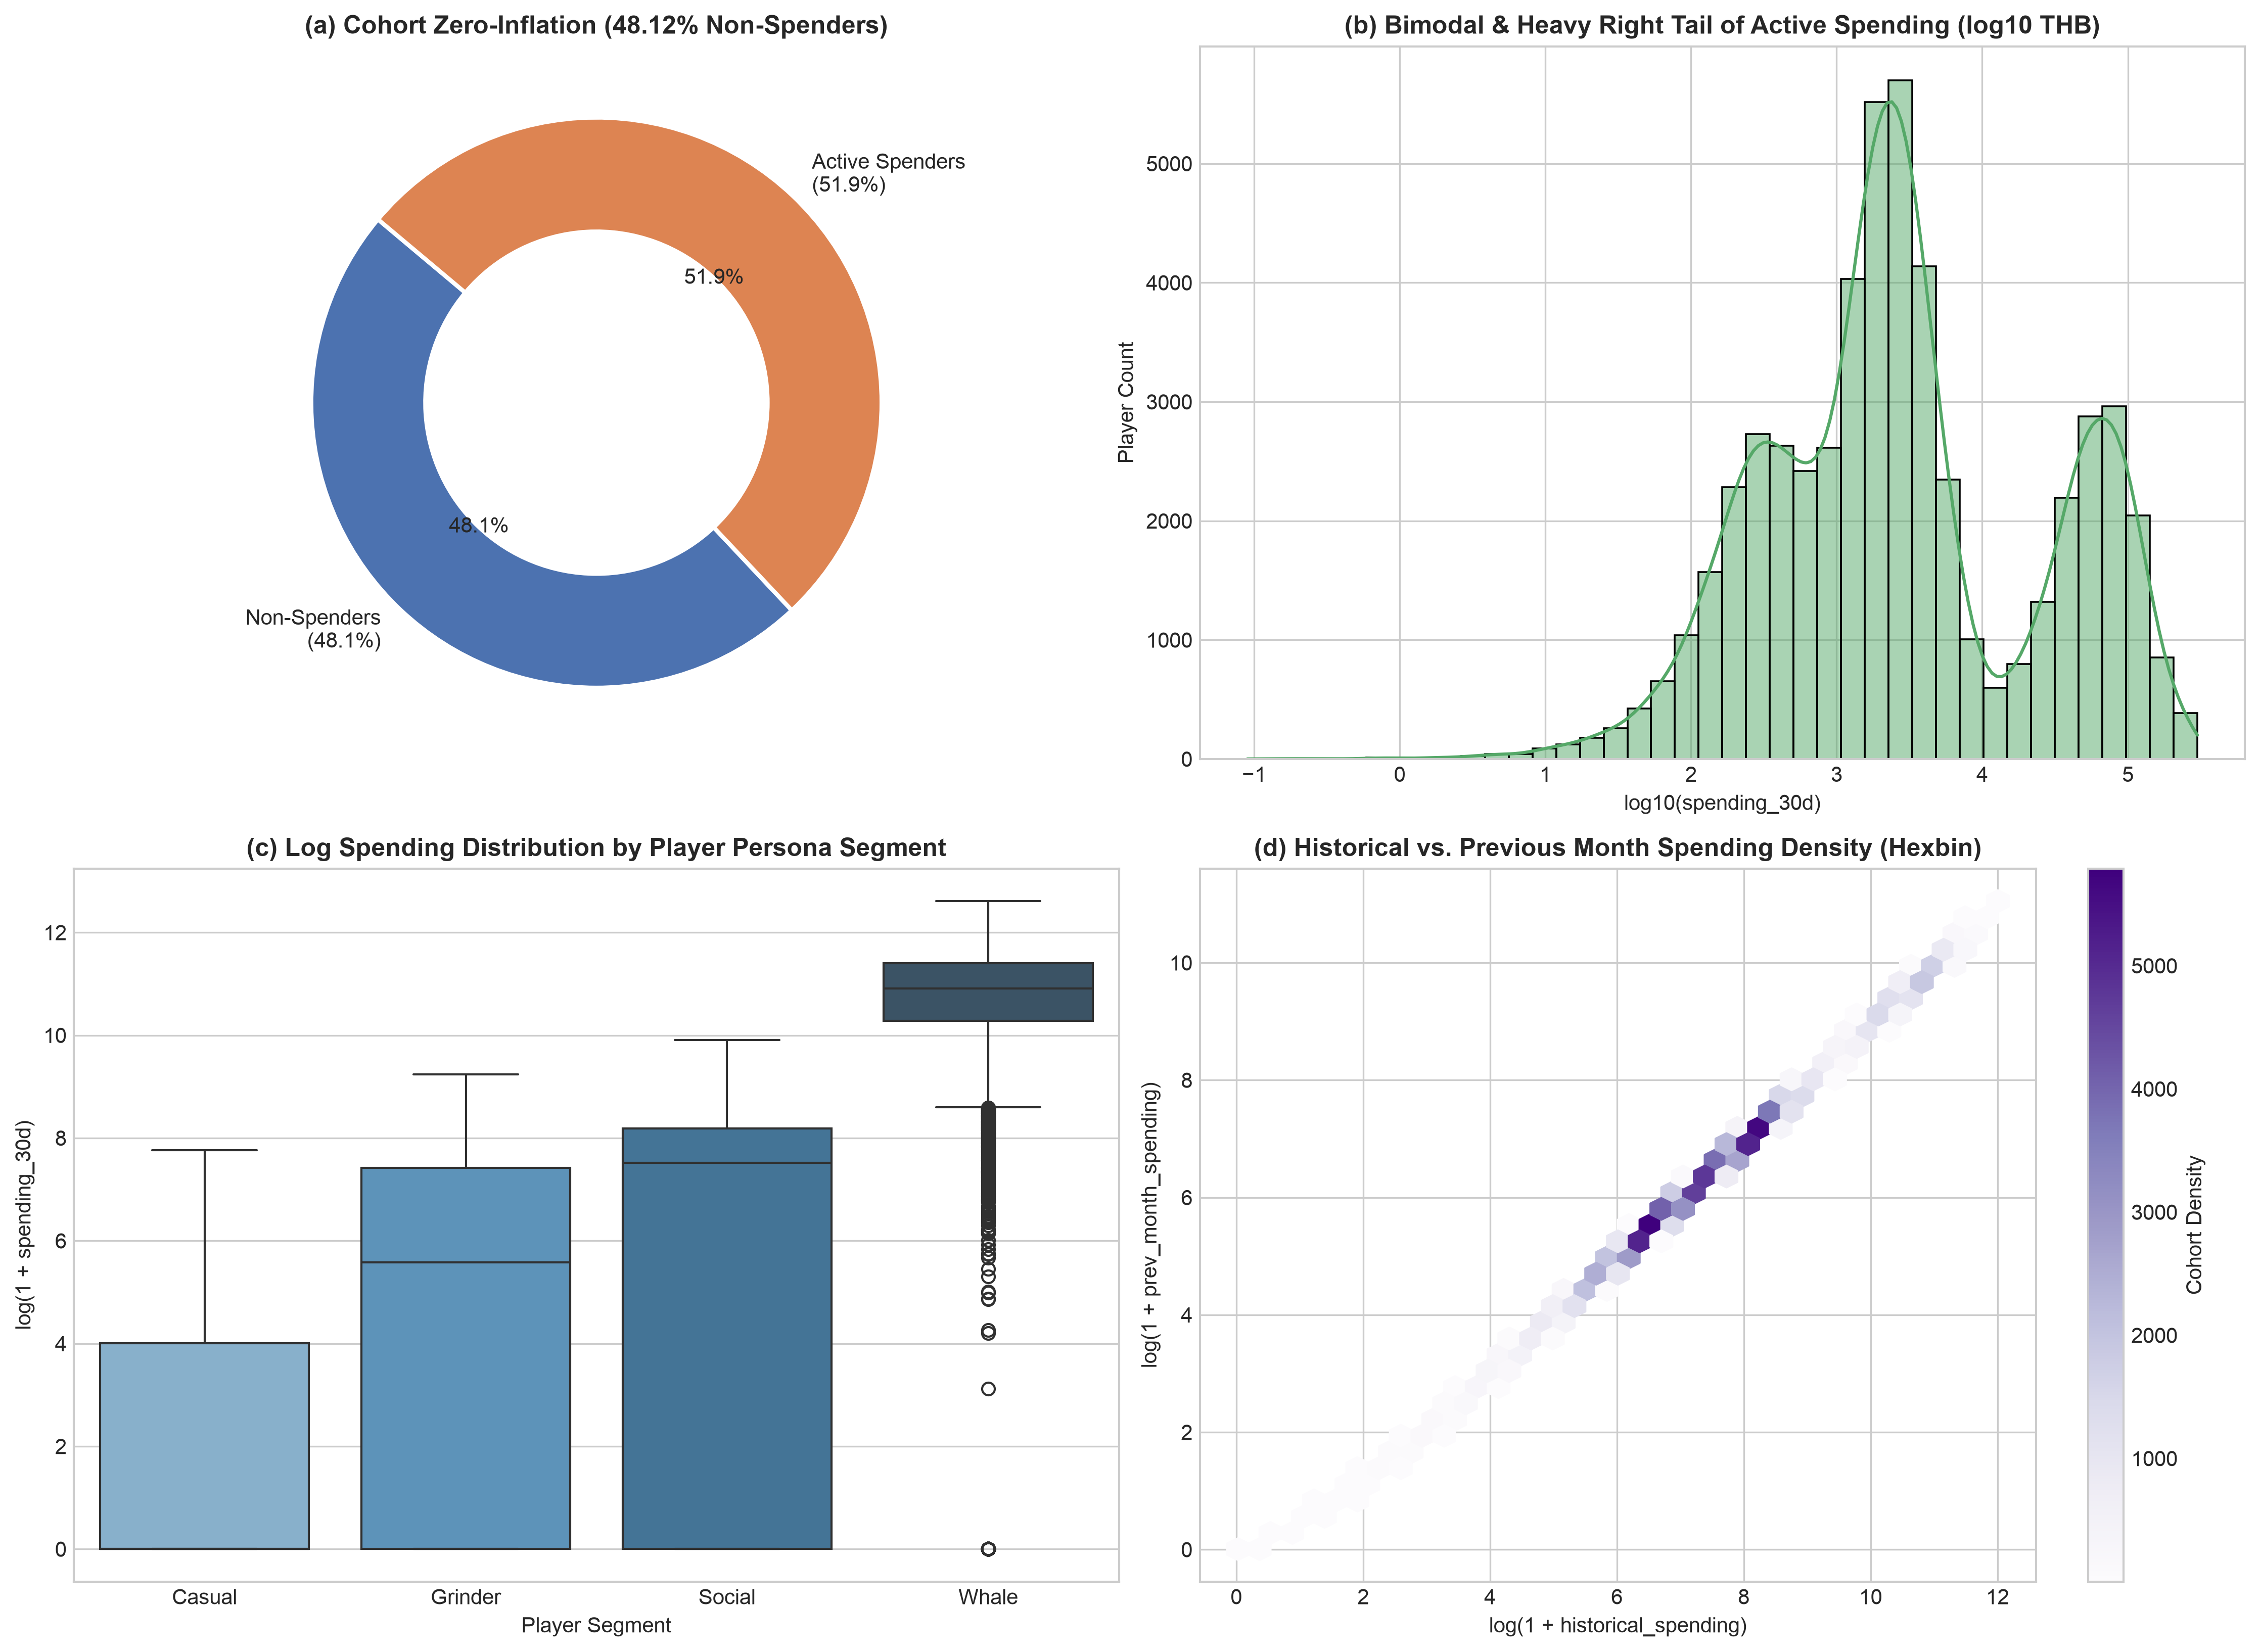
\includegraphics[width=0.92\linewidth]{assets/figure1-spending-eda.png}
\caption{การสำรวจข้อมูล Task 3: สัดส่วนผู้ไม่ใช้จ่าย 48.12\% การแจกแจงแบบสองยอดของยอดจ่ายในสเกล $\log_{10}$ ยอดจ่ายราย Segment และความสัมพันธ์กับยอดใช้จ่ายในอดีต}
\label{fig:t3_eda}
\end{figure}

\subsection{การเตรียมข้อมูลและการกู้คืนเอกลักษณ์เชิงพีชคณิต}
ดำเนินการภายใต้ 5-Fold Outer Stratified Split (จัดชั้นบนตัวแปร \code{y > 0}) พร้อม Inner 90/10 Early Stopping:
\begin{enumerate}[leftmargin=1.8em,itemsep=2pt]
    \item \textbf{Deterministic Identity Reconstruction (ความแม่นยำ 99.0\%):} ใช้กฎเอกลักษณ์ทางการเงินที่ค้นพบในข้อมูลเพื่อกู้คืนค่าว่างได้อย่างแม่นยำ ได้แก่ \code{historical\_spending = total\_transactions * avg\_transaction\_value}, \code{purchases\_on\_discount = total\_transactions * discount\_rate\_used} และ \code{is\_premium\_member = (vip\_status >= 3)} ร่วมกับค่ามัธยฐานสัดส่วนราย Fold (\code{prev\_month\_spending / historical\_spending}) ขยายฟีเจอร์สะอาดเป็น $44$ คอลัมน์
    \item \textbf{Fold-Safe Segment Recovery:} กู้คืนค่าว่างของ \code{segment} ($\sim 5.5\%$) ภายในแต่ละ Fold ด้วย Smooth-KDE Naive Bayes ร่วมกับ GBDT (\code{LogLoss = 0.1684}, ความแม่นยำราย Fold $\sim 94.2\%$)
    \item \textbf{Multiplicative Spending Law \& Huber Anchor:} บนกลุ่มผู้จ่ายเงินที่ไม่อั้นเพดาน ยอดใช้จ่ายเป็นไปตามความสัมพันธ์เชิงคูณในสเกลลอการิทึม ซึ่งประมาณค่าฐาน (Baseline Log Scale) ด้วย \code{HuberRegressor} (พารามิเตอร์ \code{epsilon=1.35}, \code{alpha=5.0}, MAE บนกลุ่ม uncapped $= 2{,}723.17$ บาท)
\end{enumerate}

\subsection{วิวัฒนาการจาก Quantile Hurdle สู่ ExactBayesL1V2}

ระบบรุ่นแรก (\code{Quantile Hurdle V3}) ประกอบด้วย Stage-1 จำนวน 6 โมเดลผสม (\code{SLSQP6}) และ Stage-2 พยากรณ์ Quantile Residuals 15 ระดับ ($0.02..0.55$) จาก 5 ตระกูลโมเดลเพื่อประเมิน $Q_{1 - 1/(2p)}$ ทำคะแนน Strict Outer OOF NMAE ได้ \code{0.795996} (MAE $2{,}690.26$ บาท) สูงกว่าค่ามัธยฐานพื้นฐาน ($0.500037$, MAE $10{,}495.48$ บาท) และ Log-Linear Ridge Hurdle ($0.646699$, MAE $5{,}734.68$ บาท)

เพื่อลดความคลาดเคลื่อนจากการแบ่ง Quantile คงที่ คณะผู้จัดทำจึงพัฒนาสถาปัตยกรรม \textbf{ExactBayesL1V2 Generative Marginalization} ซึ่งประกอบด้วย (1) ตาราง 32-Cell Exact Activation Table สำหรับ Stage-1 ที่ทำ OOF ROC-AUC $= 0.78535$ (สูงกว่า Logistic Regression $0.77614$ และ LightGBM $0.78408$), (2) กฎความหนาแน่นเชิงคูณของยอดใช้จ่าย, (3) องค์ประกอบผสม Segment-3 $\text{Uniform}[50{,}000, 300{,}000]$ และ (4) การแก้สมการหาค่ามัธยฐานมีเงื่อนไข $F_Y^{-1}(0.5 \mid X)$ โดยตรงด้วย \textbf{28-Step Bisection}

\code{ExactBayesL1V2} บรรลุ \textbf{Strict 5-Fold Outer OOF NMAE $= 0.796377$} (\textbf{MAE $= 2{,}683.96$ บาท}, เฉลี่ยราย Fold $0.796306 \pm 0.005708$) ชนะ Quantile Hurdle V3 ครบทั้ง 5 Folds ($0.786151, 0.798213, 0.799203, 0.798332, 0.799630$) ด้วยส่วนต่าง $+0.000381$ (95\% Paired Bootstrap CI \code{[+0.000212, +0.000544]}, $P = 1.0000$ จาก 1,000 รอบ) และได้รับการคัดเลือกในทุก Nested Inner Fold (\code{w\_v2=1.00, tau=0.500, scale=1.0000}) สรุปใน \textbf{ตารางที่~\ref{tab:t3_ablation}} และ \textbf{รูปที่~\ref{fig:t3_diag}}--\textbf{\ref{fig:t3_test}}

\begin{table}[H]\centering
{\fontsize{9.8}{13}\selectfont\arrayrulecolor{RuleGray}
\caption{เปรียบเทียบผล 5-Fold Strict Outer OOF Validation ของ Task 3}
\label{tab:t3_ablation}
\begin{tabular}{L{7.4cm}ccc}
\toprule
\rowcolor{TableHead} \textbf{แนวทางการสร้างแบบจำลอง (Paradigm)} & \textbf{OOF MAE (THB)} & \textbf{OOF NMAE} & \textbf{$\Delta$ vs. Median (pp)} \\
\midrule
Fold-Training Median Baseline & 10,495.48 & 0.500037 & 0.0000 \\
5-Fold Log-Linear Ridge Hurdle Baseline & 5,734.68 & 0.646699 & +14.6662 \\
Quantile Hurdle V3 (6-Stage-1 + 5-Family $Q_{\text{FINE}}$) & 2,690.26 & 0.795996 & +29.5959 \\
90\% ExactBayesL1V2 + 10\% Quantile Hurdle V3 Blend & 2,684.15 & 0.796365 & +29.6328 \\
\rowcolor{TableHead} \textbf{ExactBayesL1V2 Generative Marginalization (Final)} & \textbf{2,683.96} & \textbf{0.796377} & \textbf{+29.6340} \\
\bottomrule
\end{tabular}}
\end{table}

\begin{figure}[H]\centering
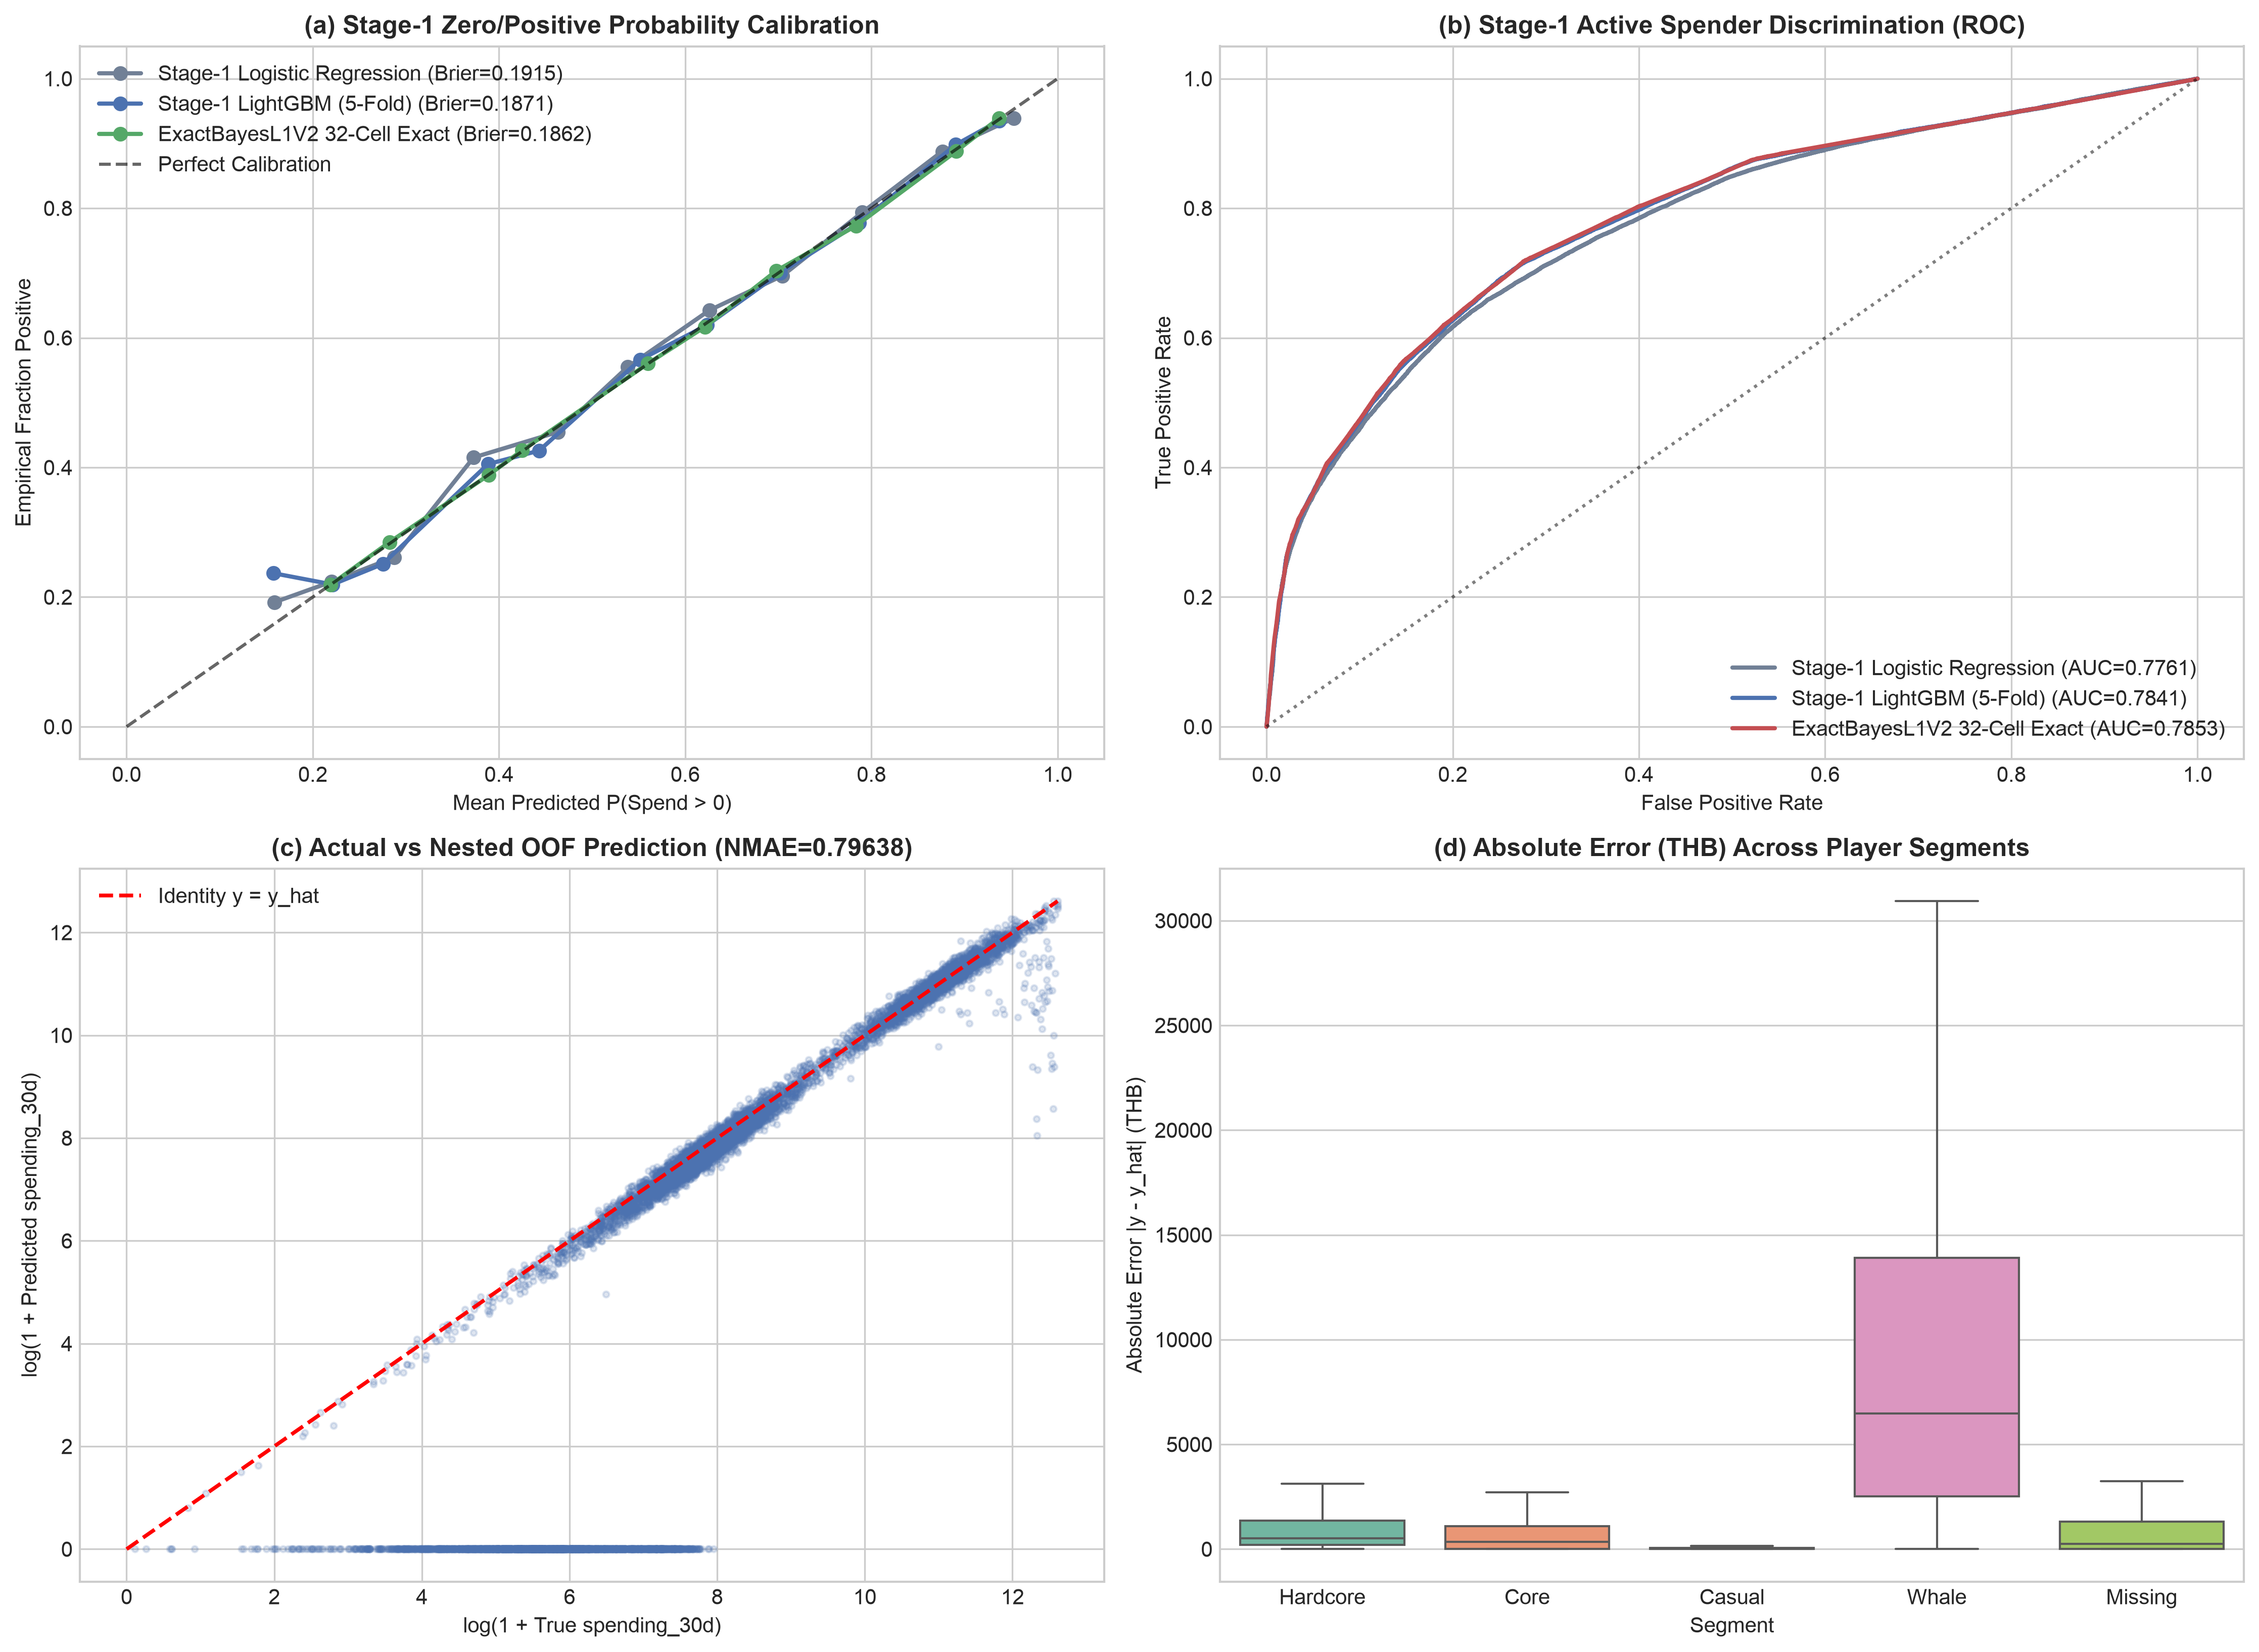
\includegraphics[width=0.95\linewidth]{assets/figure2-hurdle-calibration-diagnostics.png}
\caption{การวิเคราะห์ผล Stage-1 และ Stage-2 ของ Task 3: Reliability Calibration, Stage-1 ROC (ExactBayesL1V2 32-Cell AUC = 0.78535), Log Parity Plot และ Absolute Error ราย Segment}
\label{fig:t3_diag}
\end{figure}

\begin{figure}[H]\centering
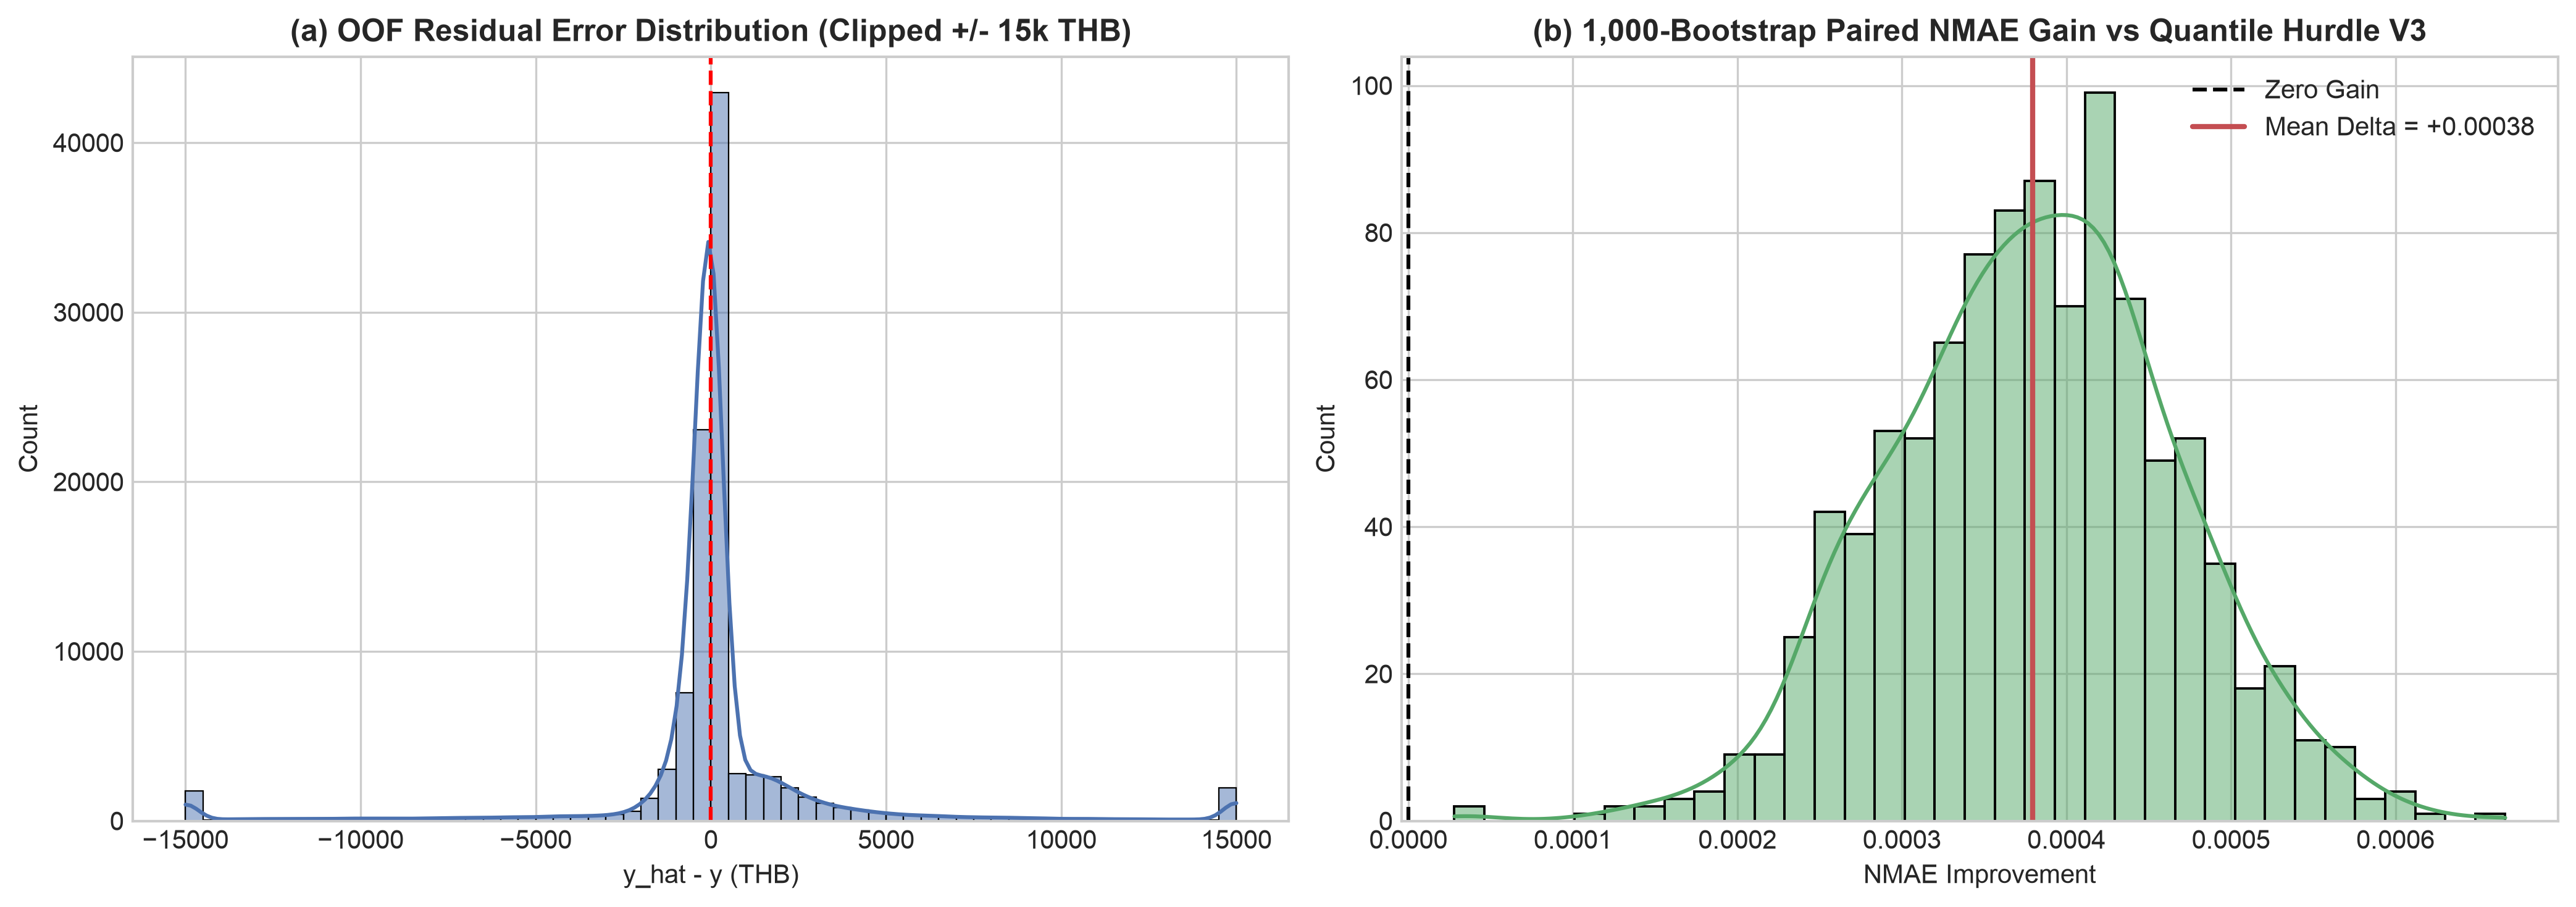
\includegraphics[width=0.92\linewidth]{assets/figure3-residual-error-distribution.png}
\caption{การกระจายตัวของค่าคลาดเคลื่อน OOF ($\pm 15\text{k}$ THB) และฮิสโตแกรม 1,000-Bootstrap Gain เหนือ Quantile Hurdle V3}
\label{fig:t3_res}
\end{figure}

\begin{figure}[H]\centering
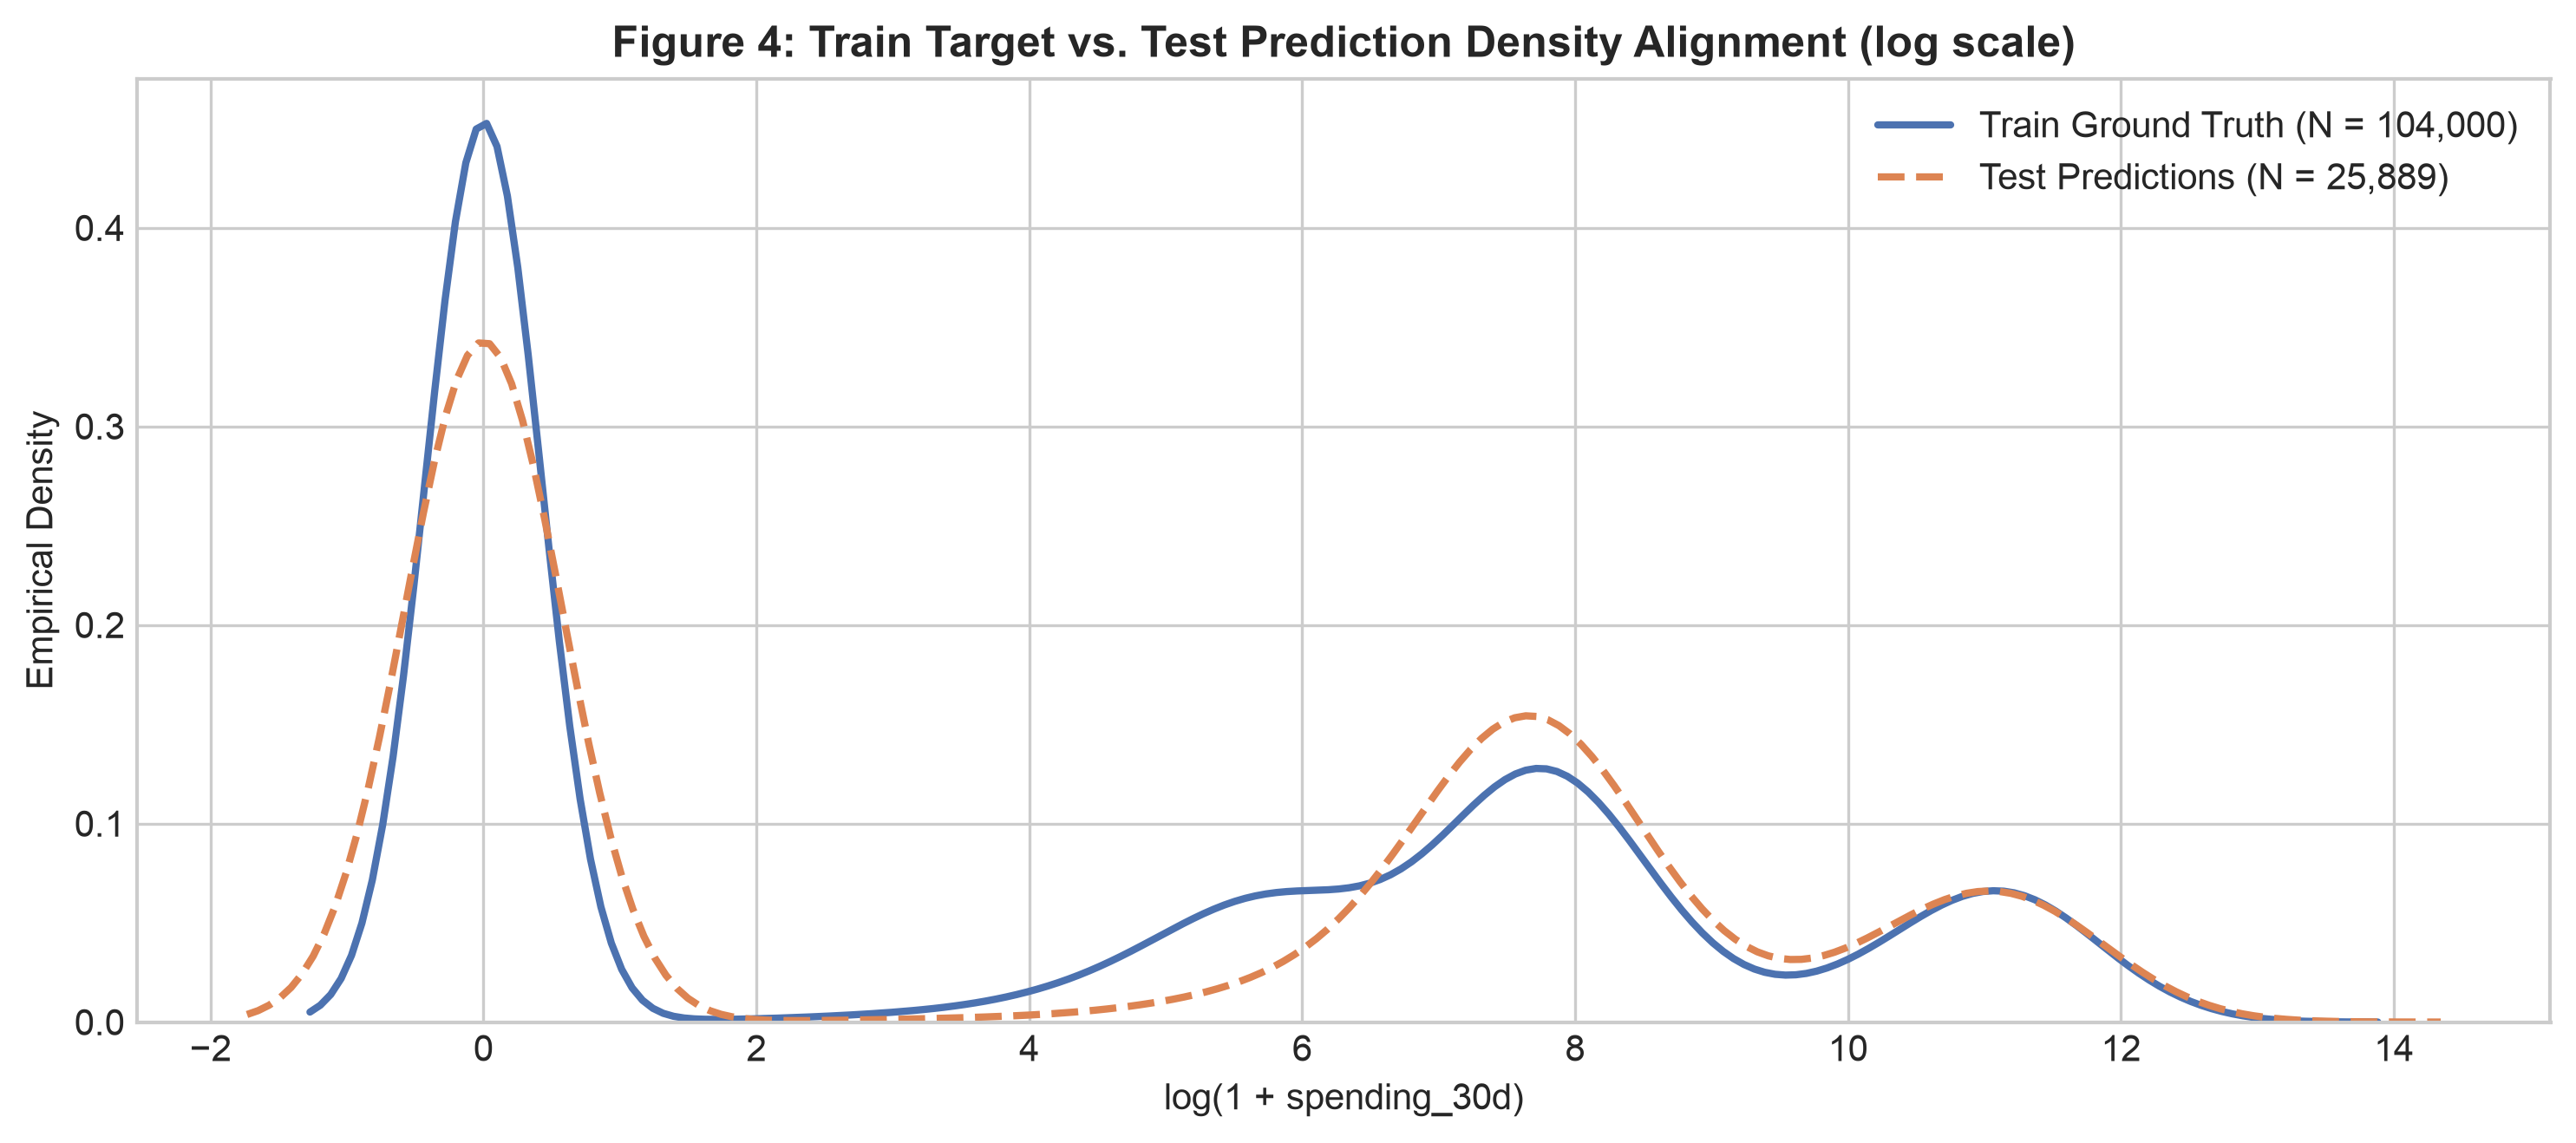
\includegraphics[width=0.88\linewidth]{assets/figure4-test-spending-prediction-density.png}
\caption{เปรียบเทียบความหนาแน่นของยอดทำนาย Test Set กับ Train Ground Truth ในสเกล Log (ทำนายศูนย์ 49.6\%, มัธยฐาน 78.76 บาท, สูงสุด 300,000 บาท)}
\label{fig:t3_test}
\end{figure}

\subsection{การวิเคราะห์ข้อผิดพลาดและผลกระทบต่อธุรกิจ}

ดังที่ปรากฏใน \textbf{รูปที่~\ref{fig:t3_diag}(d)} ค่าความคลาดเคลื่อนที่เหลืออยู่ส่วนมากมาจาก \textbf{Segment 3 (Whale)} เนื่องจากพฤติกรรมการจ่ายเงินก้อนใหญ่แบบสุ่ม $\text{Uniform}[50\text{k}, 300\text{k}]$ ไม่สามารถคาดการณ์ตัวเลขแม่นยำล่วงหน้าได้เกินกว่าค่ามัธยฐานเชิงทฤษฎี ส่วนกลุ่ม Casual, Core และ Hardcore มีความแม่นยำสูงมาก ในเชิงธุรกิจ ผลพยากรณ์บน Test Set ($49.60\%$ หรือ $12{,}841$ แถวมีค่าเท่ากับ $0.00$ บาท, ค่าเฉลี่ย $10{,}501.85$ บาท, มัธยฐาน $78.76$ บาท, รวม $271.88$ ล้านบาท) ช่วยให้ฝ่ายการเงินวางงบประมาณได้แม่นยำขึ้นและส่งต่อรายชื่อกลุ่มคาดการณ์จ่ายสูงให้ทีม VIP Support ดูแลทันที

% ==============================================================================
\clearpage
\section{Task 4: Game Title Detection (Image Classification)}

\subsection{คำอธิบายปัญหา การป้องกัน Frame Leakage และ EDA}
Task 4 จำแนกภาพหน้าจอการเล่นเกมออกเป็น 5 เกม ได้แก่ \code{0=7-11k} ($12{,}429$ ภาพ = $39.40\%$), \code{1=fiveN} ($4{,}407$ ภาพ = $13.97\%$), \code{2=freefried} ($5{,}596$ ภาพ = $17.74\%$), \code{3=pube} ($5{,}926$ ภาพ = $18.79\%$) และ \code{4=roblock} ($3{,}188$ ภาพ = $10.11\%$) รวม $31{,}546$ ภาพในชุดฝึกสอน และ $25{,}889$ ภาพในชุดทดสอบ ความละเอียด $230 \times 120$ พิกเซล RGB JPEG (\textbf{รูปที่~\ref{fig:t4_eda}}) ประเมินด้วย \textbf{Macro $F_1$} โดยอนุญาตให้ใช้ Pre-trained Vision Backbones ได้

จากการทำ EDA พบอุปสรรคสำคัญ 2 ประการ (1) การแบ่งข้อมูลแบบสุ่มปกติทำให้ภาพจากฉากเดียวกันหรือเฟรมต่อเนื่องอยู่ในทั้ง Train และ Validation ดังนั้นทีมงานจึงจัดกลุ่มภาพด้วย \textbf{Perceptual 64-bit dHash Clustering} (Hamming distance $\le 10$) แบ่งเป็น \textbf{28,088 กลุ่มฉากอิสระ} และใช้ \textbf{5-Fold StratifiedGroupKFold (SGKF)} เพื่อให้การวัดผลซื่อสัตย์ต่อภาพที่ไม่เคยเห็นจริง และ (2) พบภาพเสื่อมสภาพตามธรรมชาติ (สีเพี้ยน เอียง สัญญาณรบกวน) จำนวน $10{,}229$ ภาพ ควบคู่กับฉากเดี่ยว $7{,}931$ ภาพ จึงต้องออกแบบทั้งระบบฟื้นฟูภาพ (\code{decorrupt\_v4}) และชุดทดสอบความทนทานต่อความเสียหายขั้นรุนแรง (\code{ExtHard6})

\begin{figure}[H]\centering
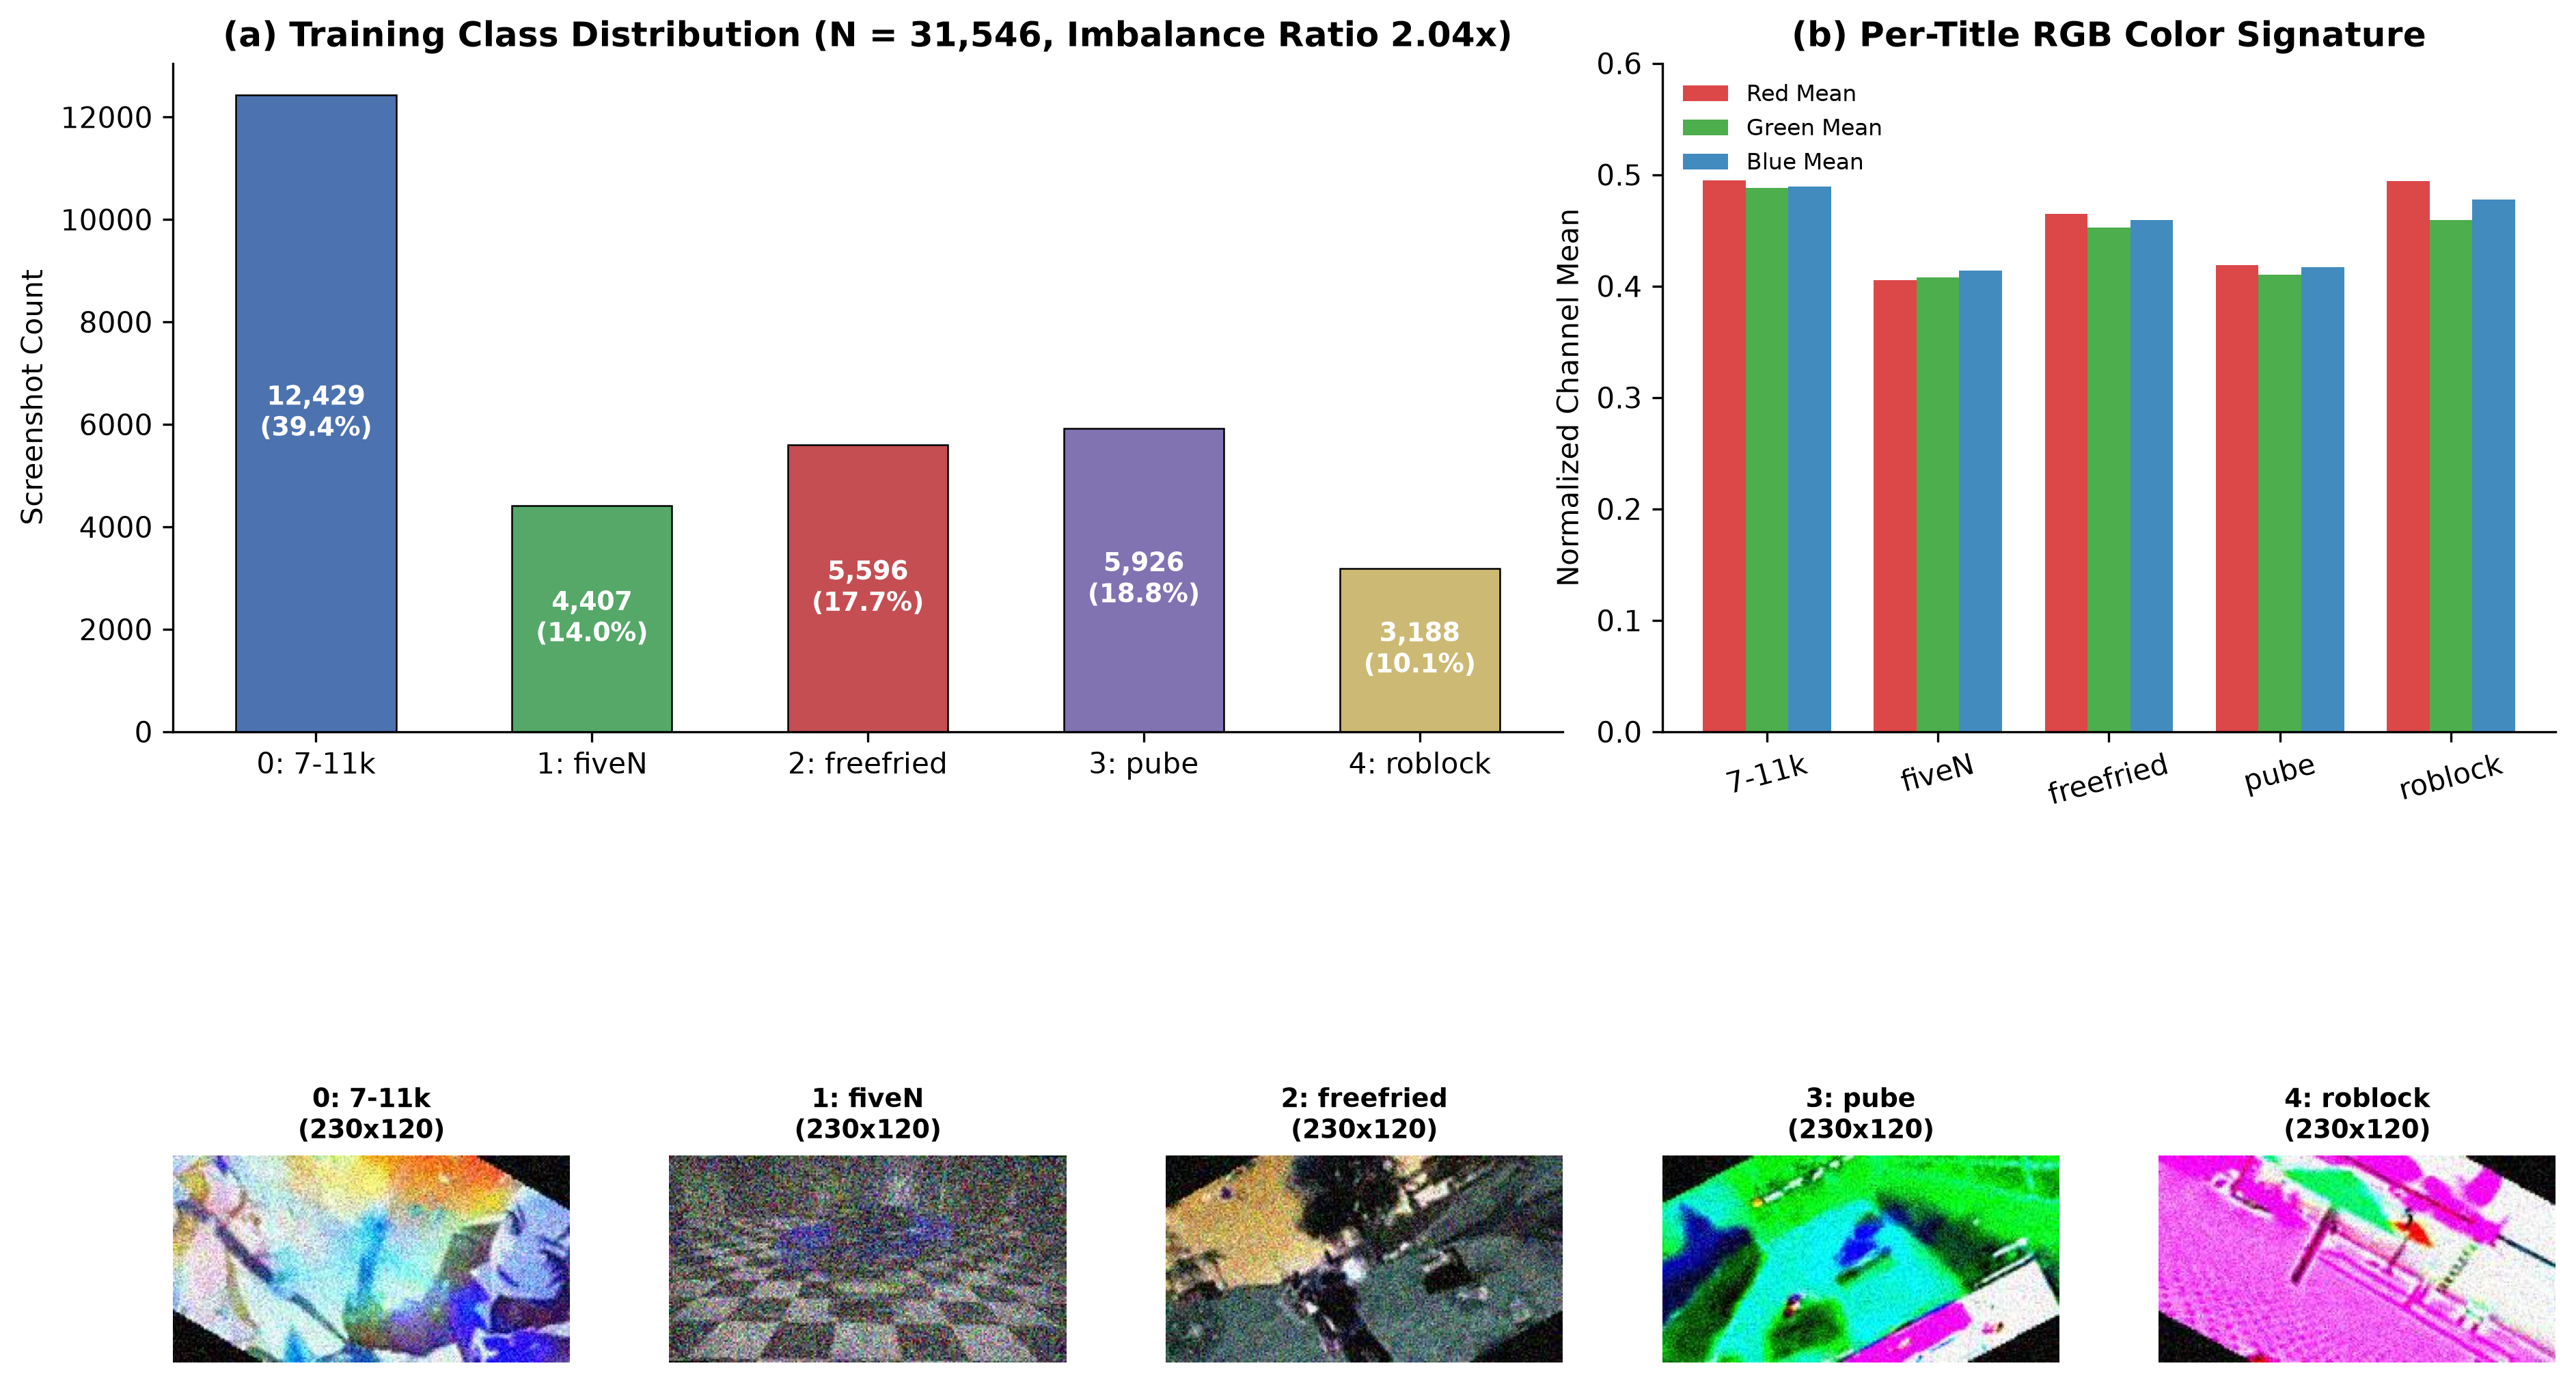
\includegraphics[width=0.92\linewidth]{assets/figure1-screenshot-eda.png}
\caption{สัดส่วนคลาสทั้ง 5 เกมในชุดฝึกสอน Task 4 (31,546 ภาพ, อัตราส่วนไม่สมดุล 2.04 เท่า) ค่าเฉลี่ยสี RGB และภาพตัวอย่างขนาด $230 \times 120$ พิกเซล}
\label{fig:t4_eda}
\end{figure}

\subsection{สถาปัตยกรรมหลายตระกูลและ Dual-Regime Log-Odds Fusion}

คณะผู้จัดทำพัฒนาโครงข่ายประมวลผลภาพ 2 ตระกูลหลักภายใต้ 5-Fold SGKF ล้วน ดังนี้:
\begin{enumerate}[leftmargin=1.8em,itemsep=2pt]
    \item \textbf{Scene-Hardened End-to-End Fine-Tuned Backbones:} ฝึกสอนโมเดลที่ความละเอียดเต็มสัดส่วน ($192 \times 384$ พิกเซล) ประกอบด้วย \code{CNXv3-Base}, \code{DINOv3L-Hard} และ \code{EVA02L-Hard} ประเมินทั้งแบบ 2-view ปกติ (\code{Orig2}) และ 6-view ฟื้นฟูภาพ (\code{Hard6 / ExtHard6}) ร่วมกับโมเดล ViT ขนาด $224$ พิกเซล (\code{EVA02-Large}, \code{EVA02-Base}, \code{DINOv3-ViT-L}, \code{DINOv3-ViT-B}) และ \code{ConvNeXtV2-Tiny} / \code{DINOv2-StageA/C}
    \item \textbf{Joint 12-Block 6-Backbone Foundation Engine (\code{FoundVLM-v3-Joint12Blk}):} สกัดเวกเตอร์ Embedding 4 มุมมอง (\code{raw}, \code{raw+hflip}, \code{decorrupt\_v4}, \code{decorrupt\_v4+hflip}) จากโมเดลฐาน 6 สถาปัตยกรรม (\code{SigLIP2-SO400M}, \code{DINOv3-ViT-L}, \code{DINOv2-ViT-G/14}, \code{CLIP-ConvNeXt-Large}, \code{CLIP-ViT-H/14}, \code{DINOv3-ConvNeXt-Base}) ต่อรวมเป็นเวกเตอร์ $13{,}568$ มิติ ปรับมาตรฐานด้วย PowerNorm ($p=0.75$) ผ่าน Dual-Condition \code{CosineResMLP} ที่บังคับความคงที่ระหว่างภาพดิบกับภาพฟื้นฟูด้วย Symmetric-KL Consistency Loss
\end{enumerate}

ขั้นตอนผสานผลใช้ \textbf{Nested Temperature-Calibrated Log-Odds Geometric Pooling} สองสภาวะ คือ \textbf{Clean Pool} (11 Active Streams) และ \textbf{Unconstrained \code{ExtHard6} Pool} (กำหนด \code{min\_bound = 0.00} ทำให้ลดน้ำหนัก \code{DINOv2-StageC-6TTA} ที่มีสัญญาณรบกวนลงเหลือ $0.0000$ โดยอัตโนมัติ และเน้นน้ำหนักไปที่ \code{FoundVLM-4Fam-Hard6} $0.2607$, \code{CNXv2-StageC-6TTA} $0.2321$, \code{EVA02L-Hard-Hard6} $0.2302$ และ \code{DINOv3L-Hard-Hard6} $0.2170$) ควบคุมการสลับด้วย \textbf{Consensus Restoration Shift Gate} (ใช้เกณฑ์ Jensen-Shannon Divergence $\text{JS}(\text{Orig2}, \text{Hard6}) > \tau_{98\%} = 0.004910$ และเอนโทรปีที่ลดลง ที่สัดส่วน $\gamma = 0.04$ คัดส่ง $795$ ภาพบน Test Set) พร้อม Prior Debiasing ($\alpha_{\text{lo}}=0.69 \to \alpha_{\text{hi}}=1.35$) ทำให้ได้ \textbf{Clean Unif-Prior Macro-$F_1 = 0.994636$}, All OOF $F_1 = 0.994054$, Corrupt $F_1 = 0.989205$, \textbf{ExtHard6 $F_1 = 0.969820$} และ OOF LogLoss $= 0.019164$ (\textbf{ตารางที่~\ref{tab:t4_ablation}}, \textbf{ตารางที่~\ref{tab:t4_perclass}} และ \textbf{รูปที่~\ref{fig:t4_diag}}--\textbf{\ref{fig:t4_test}})

\begin{table}[H]\centering
{\fontsize{9.2}{12.2}\selectfont\arrayrulecolor{RuleGray}
\caption{เปรียบเทียบผลวิวัฒนาการของโมเดล Task 4 ภายใต้ 5-Fold SGKF (Stage 1--5)}
\label{tab:t4_ablation}
\begin{tabular}{L{7.6cm}ccc}
\toprule
\rowcolor{TableHead} \textbf{โมเดล / ขั้นตอนการพัฒนา} & \textbf{Clean Unif $F_1$} & \textbf{ExtHard6 $F_1$} & \textbf{OOF LogLoss} \\
\midrule
Individual: Base ViT EVA02-Large (224px) & 0.989078 & --- & 0.069633 \\
Individual: Full-Res CNXv3-Base ($192 \times 384$ Hard6) & 0.988908 & 0.950293 & 0.053564 \\
Individual: Full-Res DINOv3L-Hard ($192 \times 384$ Hard6) & 0.991634 & 0.959898 & 0.048022 \\
Individual: Full-Res EVA02L-Hard ($192 \times 384$ Hard6) & 0.991497 & 0.959546 & 0.048044 \\
Individual: FoundVLM-v3-Joint12Blk (6-BB 13,568d) & 0.968200 & 0.925210 & 0.101140 \\
Stage 1: 9-Stream Base (E2E + ViTs + DINOv2) & 0.991313 & --- & 0.026300 \\
Stage 2: Hardened Trio + Restoration Shift Gate & 0.994412 & 0.968800 & 0.019381 \\
Stage 3: + 5-Backbone De-Corrupted FoundVLM-v1 & 0.994567 & 0.968804 & 0.018961 \\
Stage 4: + Dual-Condition SymKL FoundVLM-v2 & 0.994573 & 0.969549 & 0.019192 \\
\rowcolor{TableHead} \textbf{Stage 5 (Final): + Joint-12Blk \& Unconstrained ExtHard6} & \textbf{0.994636} & \textbf{0.969820} & \textbf{0.019164} \\
\bottomrule
\end{tabular}}
\end{table}

\begin{table}[H]\centering
{\fontsize{9.0}{12}\selectfont\setlength{\tabcolsep}{4.5pt}\arrayrulecolor{RuleGray}
\caption{ประสิทธิภาพรายเกมของโมเดลขั้นสุดท้าย Task 4 และสัดส่วนการทำนายบน Test Set (25,889 ภาพ)}
\label{tab:t4_perclass}
\begin{tabular}{clcccccc}
\toprule
\rowcolor{TableHead} \textbf{ID} & \textbf{ชื่อเกม (Slug)} & \textbf{Support} & \textbf{Clean Prec} & \textbf{Clean Rec} & \textbf{Clean $F_1$} & \textbf{ExtHard6 $F_1$} & \textbf{Test Predicted} \\
\midrule
0 & 7-11 Knights (\code{7-11k}) & 12,429 & 0.9970 & 0.9961 & 0.9966 & 0.9830 & 3,575 (13.81\%) \\
1 & FiveN (\code{fiveN}) & 4,407 & 0.9961 & 0.9930 & 0.9945 & 0.9737 & 6,790 (26.23\%) \\
2 & Free Fried (\code{freefried}) & 5,596 & 0.9957 & 0.9950 & 0.9954 & 0.9722 & 3,932 (15.19\%) \\
3 & PUBE (\code{pube}) & 5,926 & 0.9959 & 0.9941 & 0.9950 & 0.9704 & 6,278 (24.25\%) \\
4 & Roblock (\code{roblock}) & 3,188 & 0.9827 & 0.9950 & 0.9888 & 0.9549 & 5,314 (20.53\%) \\
\bottomrule
\end{tabular}}
\end{table}

\begin{figure}[H]\centering
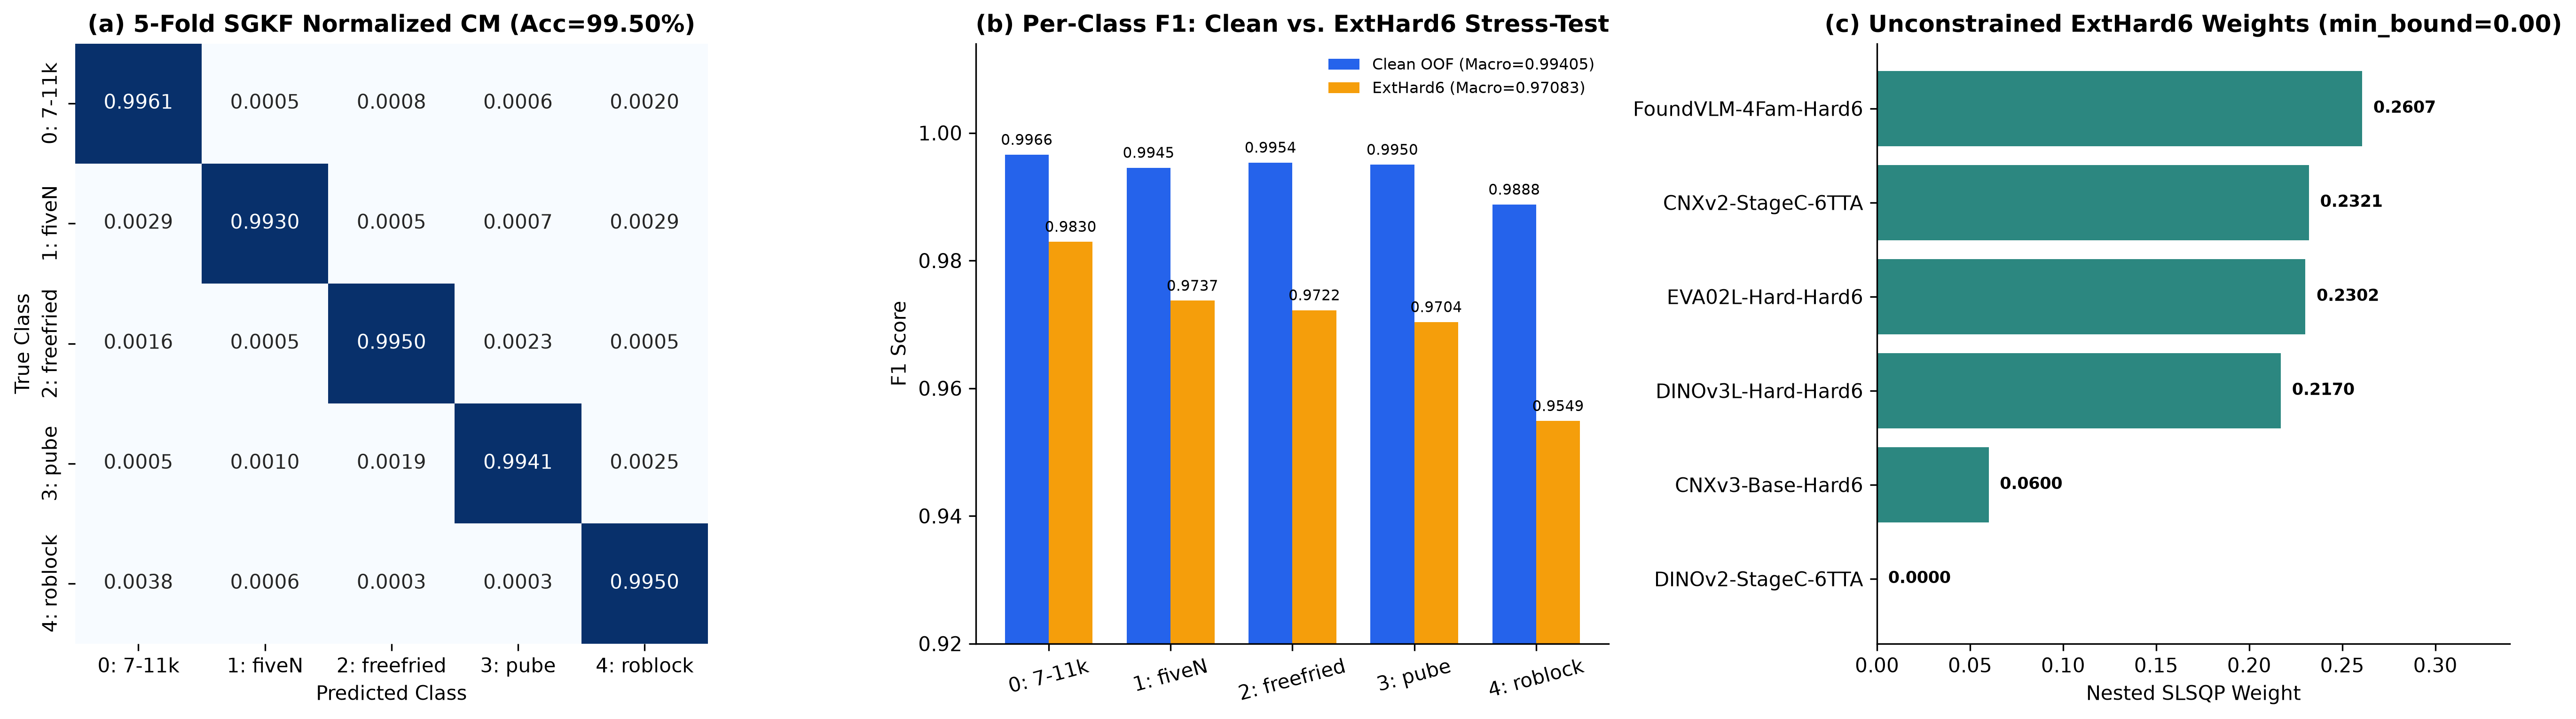
\includegraphics[width=0.95\linewidth]{assets/figure2-validation-diagnostics.png}
\caption{ผลการประเมิน 5-Fold SGKF ของ Task 4: เมทริกซ์ความสับสน (Accuracy 99.50\%) ค่า $F_1$ รายเกมในโหมดปกติกับ ExtHard6 และน้ำหนัก SLSQP ในกลุ่ม ExtHard6}
\label{fig:t4_diag}
\end{figure}

\begin{figure}[H]\centering
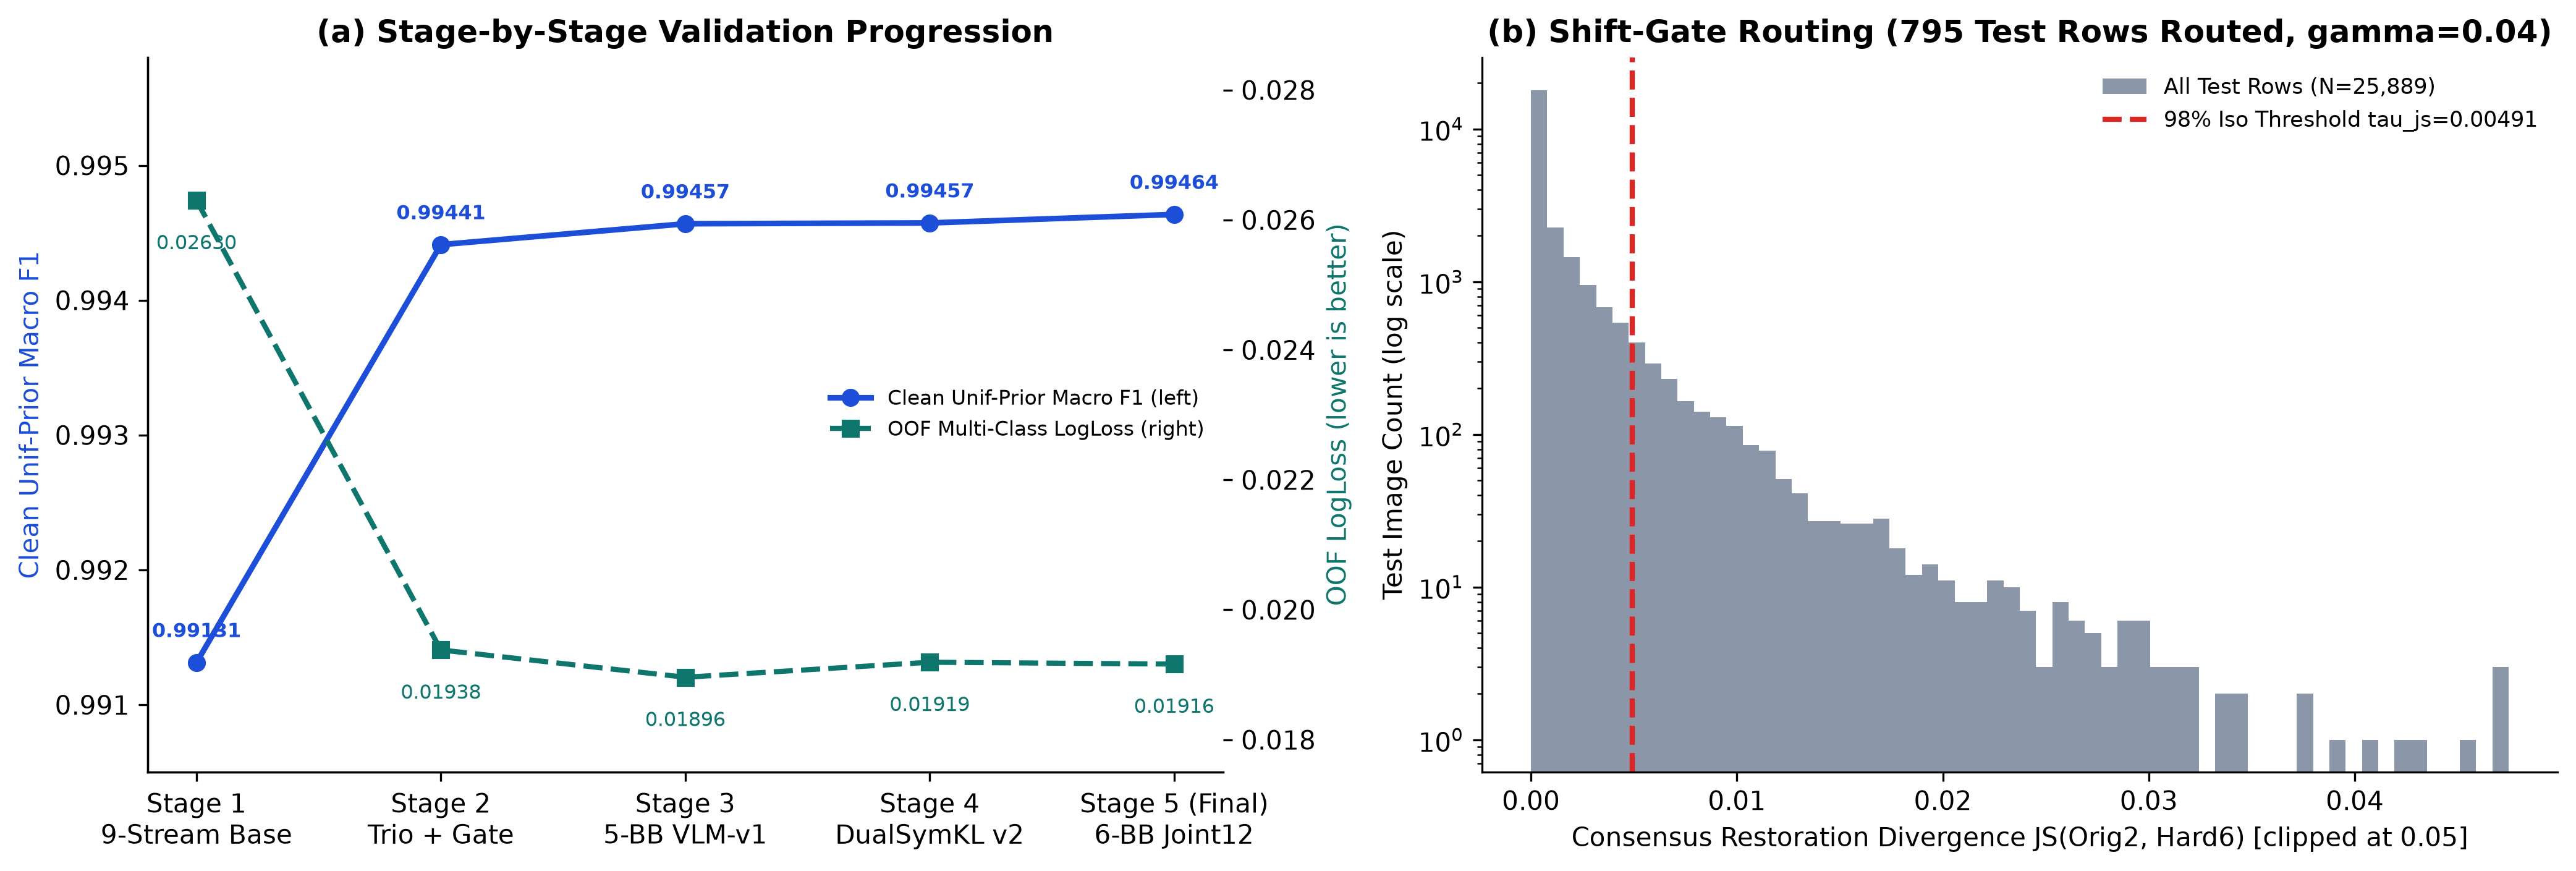
\includegraphics[width=0.94\linewidth]{assets/figure3-regime-error-analysis.png}
\caption{พัฒนาการความแม่นยำ Stage 1--5 ของ Task 4 และการกระจายตัวของ JS Divergence ใน Shift Gate ($\gamma = 0.04$, คัดส่ง 795 ภาพ)}
\label{fig:t4_regime}
\end{figure}

\begin{figure}[H]\centering
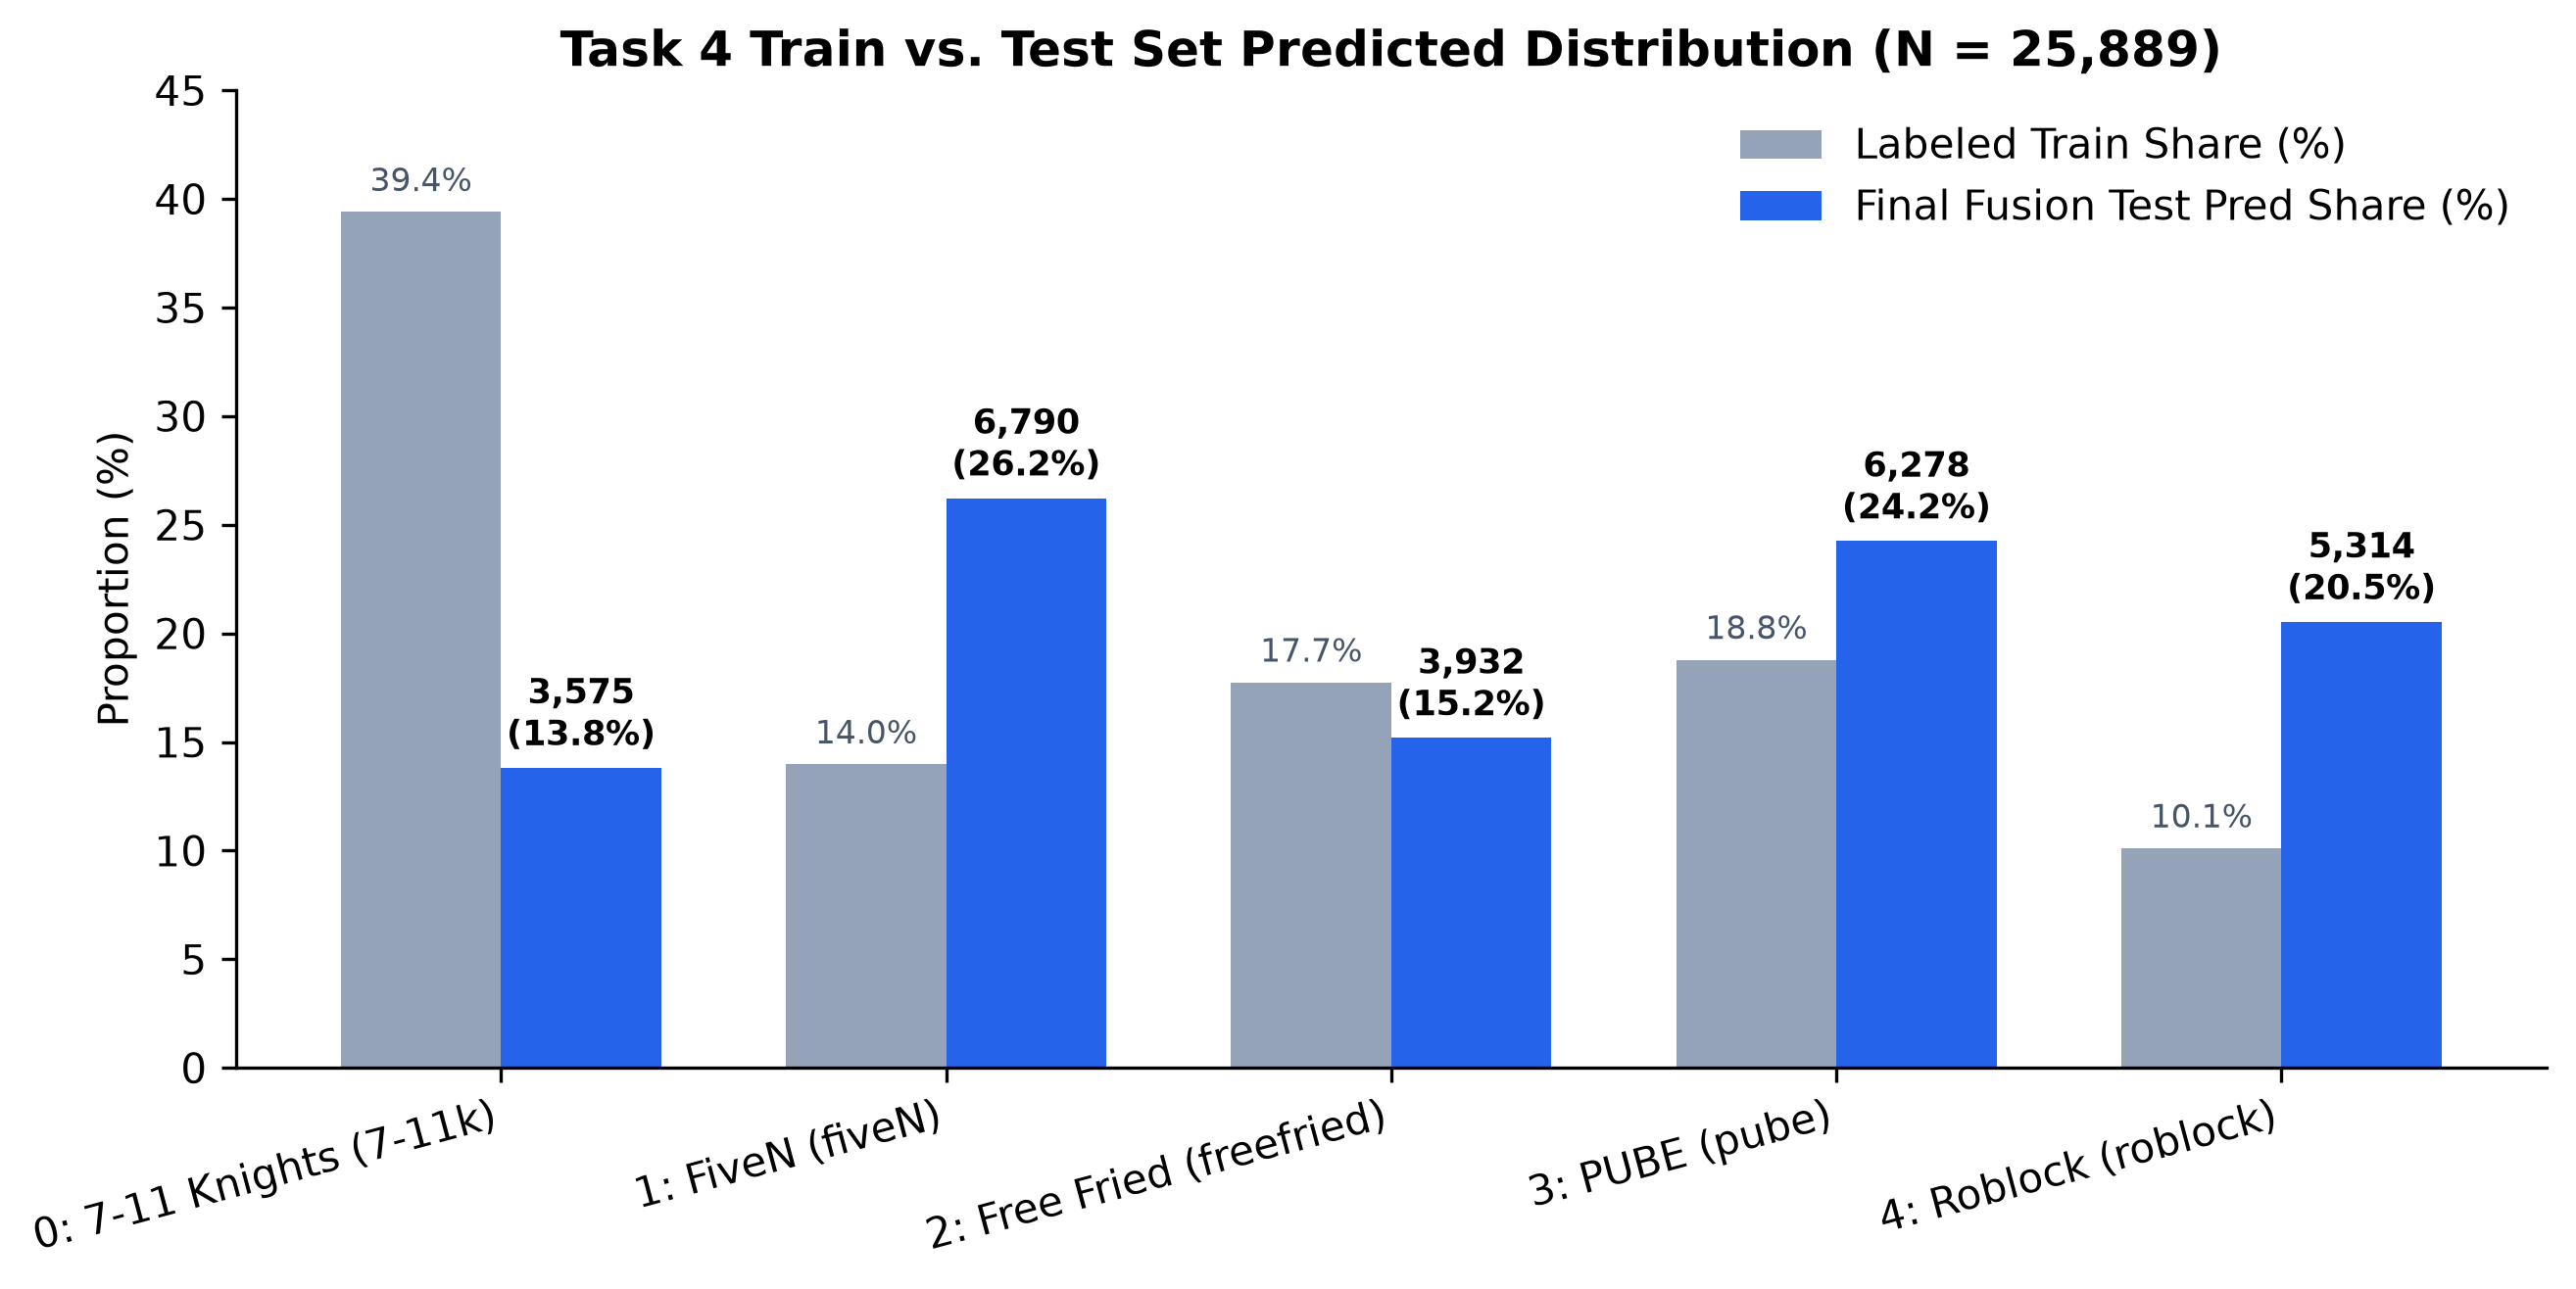
\includegraphics[width=0.86\linewidth]{assets/figure4-test-class-distribution.png}
\caption{เปรียบเทียบสัดส่วนคลาสทั้ง 5 เกมระหว่าง Train Set กับผลการทำนายบน Test Set (25,889 ภาพ)}
\label{fig:t4_test}
\end{figure}

\subsection{การวิเคราะห์ข้อผิดพลาดและผลกระทบต่อธุรกิจ}

ระหว่างพัฒนาพบกรณีศึกษาที่ส่งผลลบต่อการจำแนก 2 ประการ คือ (1) โมเดลความละเอียดต่ำ (\code{ConvNeXtV2-StageC} เพียงตัวเดียว) ทำให้สูญเสียรายละเอียด HUD และอินเทอร์เฟซของเกม และการกำหนดค่า Shift Gate รุกเกินไป ($\gamma = 0.08$) ส่งผลให้ภาพหน้าจอปกติบางส่วนถูกส่งผ่านไปประมวลผลแบบภาพเสียหาย การล็อก $\gamma = 0.04$ และปล่อยให้ SLSQP ปรับน้ำหนัก \code{DINOv2-StageC} เป็น $0.0000$ จึงช่วยรักษาความแม่นยำทั้งภาพสะอาดและภาพเสียหายได้พร้อมกัน

จากการเปรียบเทียบใน \textbf{รูปที่~\ref{fig:t4_test}} พบว่า Test Set มีการเปลี่ยนแปลงสัดส่วนเกมจาก Train Set อย่างชัดเจน (เช่น \textit{7-11 Knights} ลดจาก $39.4\%$ เหลือ $13.8\%$ ขณะที่ \textit{FiveN} และ \textit{Roblock} เพิ่มเป็น $26.2\%$ และ $20.5\%$) โมเดลที่ผ่านการปรับเทียบจึงสามารถคัดแยกตั๋วแจ้งปัญหา 2,000 ใบต่อวันและตรวจภาพกิจกรรม 50,000+ ภาพได้อย่างแม่นยำเกิน $99\%$ ในเกือบทุกเกม ลดเวลาทำงานเจ้าหน้าที่จาก 10 นาทีต่อใบลงสู่ระบบอัตโนมัติ

% ==============================================================================
\clearpage
\section{Task 5: Account Security Monitoring (Unsupervised Anomaly Detection)}

\subsection{คำอธิบายปัญหาและข้อจำกัดของวิธี Unsupervised มาตรฐาน}
Task 5 เป็นงานตรวจจับบัญชีผิดปกติ (\code{is\_anomaly = 1}) ภายใต้มาตรวัด \textbf{$F_3$ Score} ในสภาวะ \textbf{Unsupervised Pure-Test} โดยชุดข้อมูลมีเฉพาะ \code{test.csv} ขนาด $25{,}889 \times 123$ คอลัมน์ ปราศจากป้ายกำกับ ภายในประกอบด้วยตัวแปรพฤติกรรมระยะยาว 29 ตระกูล วัดผล 4 ช่วงเวลา (\code{\_1..\_4}), \code{account\_age\_days}, \code{behavior\_stability} และธงความมั่นคงปลอดภัย 4 ตัว (\code{password\_changed}, \code{vpn\_usage}, \code{suspicious\_login\_time}, \code{mass\_item\_sale}) ซึ่งทีมผู้พัฒนา \textbf{กันออกจากการสร้างแบบจำลองโดยสิ้นเชิง} เพื่อใช้ทวนสอบความน่าเชื่อถือในขั้นตอนสุดท้าย

ข้อค้นพบสำคัญคือ อัลกอริทึมระยะทางบนปริภูมิรวมทั้งหมด (Full-Space Detectors) เช่น Isolation Forest มาตรฐาน หรือ Dense Autoencoder ประสบปัญหา Feature Dilution เนื่องจากบัญชีที่ผิดปกติจริงมักแสดงความผิดปกติรุนแรงบนฟีเจอร์เฉพาะทางเพียง 1--4 ตัวแปร จากกว่า 75+ มิติ ขณะที่ตัวแปรอื่นทั้งหมดยังอยู่ในเกณฑ์ปกติ

\subsection{วิศวกรรมความเบี่ยงเบนเฉพาะบุคคลและกฎ 8 Archetypes}

ทีมงานแปลงอนุกรมเวลา 4 ช่วงเวลาเป็นตัวแปรเปรียบเทียบตนเองเพื่อดึงสัญญาณความผิดปกติออกมาให้ชัดเจน ได้แก่ \textbf{Personal Drift (\code{\_\_drift4})} (ช่วงที่ 4 ลบค่ามัธยฐานช่วง 1--3), \textbf{Population Level \& Spread (\code{\_\_level}, \code{\_\_spread})} สำหรับตรวจบอตที่มีพฤติกรรมซ้ำเดิมผิดธรรมชาติ และ \textbf{Geo Displacement (\code{geo\_\_disp4}, \code{geo\_\_disp\_max})} วัดระยะการเปลี่ยนพิกัดล็อกอินโดยรองรับเส้นแบ่งเขตวัน

เมื่อประยุกต์ \textbf{1D Density-Gap CBLOF ($\ge 100\times$ Core Spacing)} และ \textbf{Soft-Max Robust Tail Score} ($\tau > 18.35$ ครอบคลุม 826 บัญชีปลายหาง) ร่วมกับการค้นหาช่องว่างความหนาแน่น พบกลุ่มความผิดปกติที่แยกตัวจากกลุ่มปกติอย่างเด็ดขาด 7 กลุ่มฟีเจอร์เดี่ยว (เช่น \code{behavior\_stability} มีช่องว่างห่างจากกลุ่มหลักถึง $38{,}792.1\times$) ผสานกับกล่องไฮเปอร์สี่เหลี่ยม 12 มิติสำหรับกลุ่มที่ 8 คือ \code{erratic\_combat} (\code{kda\_std} $\in [0.7, 1.0]$, \code{accuracy\_std} $\in [9.0, 12.0]$, \code{performance\_stability} $\in [0.85, 0.95]$ ที่สังเกต $\ge 6$ คาบ, \textbf{รูปที่~\ref{fig:t5_box}}) สามารถแยกบัญชีผิดปกติแบบชัดเจนได้ \textbf{2,052 บัญชี (7.93\%)}

\subsection{การกู้คืนบัญชี Unstable Behavior ด้วย ExactBayesUB}

ในกลุ่มบัญชีที่ตัวแปร \code{behavior\_stability} ขาดหาย (\code{NaN} $\sim 5\%$) ทีมงานแทนที่โมเดลต้นไม้ (LightGBM/CatBoost) ด้วยแบบจำลองความน่าจะเป็นเชิงวิเคราะห์แบบไร้พารามิเตอร์ฝึกสอนชื่อ \textbf{ExactBayesUB} บนตัวกรองเบื้องต้น (\code{purchase\_frequency} $\in [3, 6]$, \code{account\_age\_days} $\ge 795$) โดยอินทิเกรตความหนาแน่นร่วมแบบ Closed-Form ของพฤติกรรมปกติเทียบกับ Unstable เหนือ \code{purchase\_frequency\_1..4}, \code{login\_count\_1..4} (ใช้ 200-Point Gauss-Legendre Quadrature) และ \code{account\_age\_days}

เมื่อทำ Masked Validation บนบัญชีปกติที่ทราบค่าจริง $22{,}926$ ราย ($2{,}393$ รายผ่านตัวกรองเบื้องต้น, $246$ รายผิดปกติ) \code{ExactBayesUB} ทำคะแนน \textbf{Masked ROC-AUC $= 0.9940$} ($0.93656$ ภายในตัวกรอง $2{,}393$ แถว เทียบ $0.91251$ ของ LightGBM เดิม) และ \textbf{PR-AUC $= 0.7992$} เมื่อเลือกจุดตัดที่เพิ่มค่า Expected-$F_3$ สูงสุดได้จุดตัด \code{0.11513} ซึ่งกู้คืนบัญชีซ่อนเร้นได้เพิ่มอีก \textbf{+25 บัญชี} รวมเป็น \textbf{2,077 / 25,889 บัญชี (8.02\%)} โดยให้ค่า Expected-$F_3 = 0.99835$ ณ จุดกู้คืน 25 บัญชี (ใกล้จุดสูงสุดบนเส้นโค้งที่ \textbf{0.998363} ภายใน $10^{-5}$) สรุปผลใน \textbf{ตารางที่~\ref{tab:t5_summary}} และ \textbf{รูปที่~\ref{fig:t5_diag}}--\textbf{\ref{fig:t5_align}}

\begin{table}[H]\centering
{\fontsize{9.6}{12.5}\selectfont\arrayrulecolor{RuleGray}
\caption{สรุปจำนวนบัญชีแต่ละ Archetype และผลทวนสอบบน Security Flags ที่ซ่อนไว้ของ Task 5}
\label{tab:t5_summary}
\begin{tabular}{L{4.8cm}ccccc}
\toprule
\rowcolor{TableHead} \textbf{กลุ่มพฤติกรรม (Archetype)} & \textbf{บัญชี} & \textbf{สัดส่วน} & \textbf{เปลี่ยนรหัสผ่าน} & \textbf{ใช้ VPN} & \textbf{ขายไอเทมมาก} \\
\midrule
\code{normal} (บัญชีปกติ) & 23,812 & 91.98\% & 4.90\% & 15.26\% & 2.07\% \\
\code{account\_takeover} & 508 & 1.96\% & \textbf{61.49\%} & \textbf{50.61\%} & \textbf{43.54\%} \\
\code{account\_sale\_boosting} & 310 & 1.20\% & 5.84\% & 14.78\% & 2.40\% \\
\code{low\_activity} & 265 & 1.02\% & 5.67\% & 11.58\% & 1.23\% \\
\code{silent\_account} & 263 & 1.02\% & 5.67\% & 9.09\% & 1.98\% \\
\code{unstable\_behavior} & 246 & 0.95\% & 5.88\% & 14.22\% & 2.98\% \\
\code{erratic\_combat} (12D Box) & 244 & 0.94\% & 3.91\% & 17.09\% & 2.55\% \\
\code{bot\_24\_7} & 207 & 0.80\% & 4.12\% & 18.97\% & 1.01\% \\
\code{unstable\_behavior\_nan} & 25 & 0.10\% & 0.00\% & 8.33\% & \textbf{13.64\%} \\
\code{vpn\_pricing\_abuse} (เฉพาะกลุ่ม) & 9 & 0.03\% & 11.11\% & \textbf{100.00\%} & 0.00\% \\
\bottomrule
\end{tabular}}
\end{table}

\textit{หมายเหตุ:} กฎ \code{vpn\_pricing\_abuse} (\code{purchase\_frequency\_4 > 7.5}) มีบัญชีที่เข้าเงื่อนไขรวม $189$ บัญชี แต่ $180$ บัญชีซ้อนทับกับ \code{account\_takeover} จึงคงเหลือในตารางลำดับชั้นอิสระไม่ซ้ำซ้อนจำนวน $9$ บัญชี

\begin{figure}[H]\centering
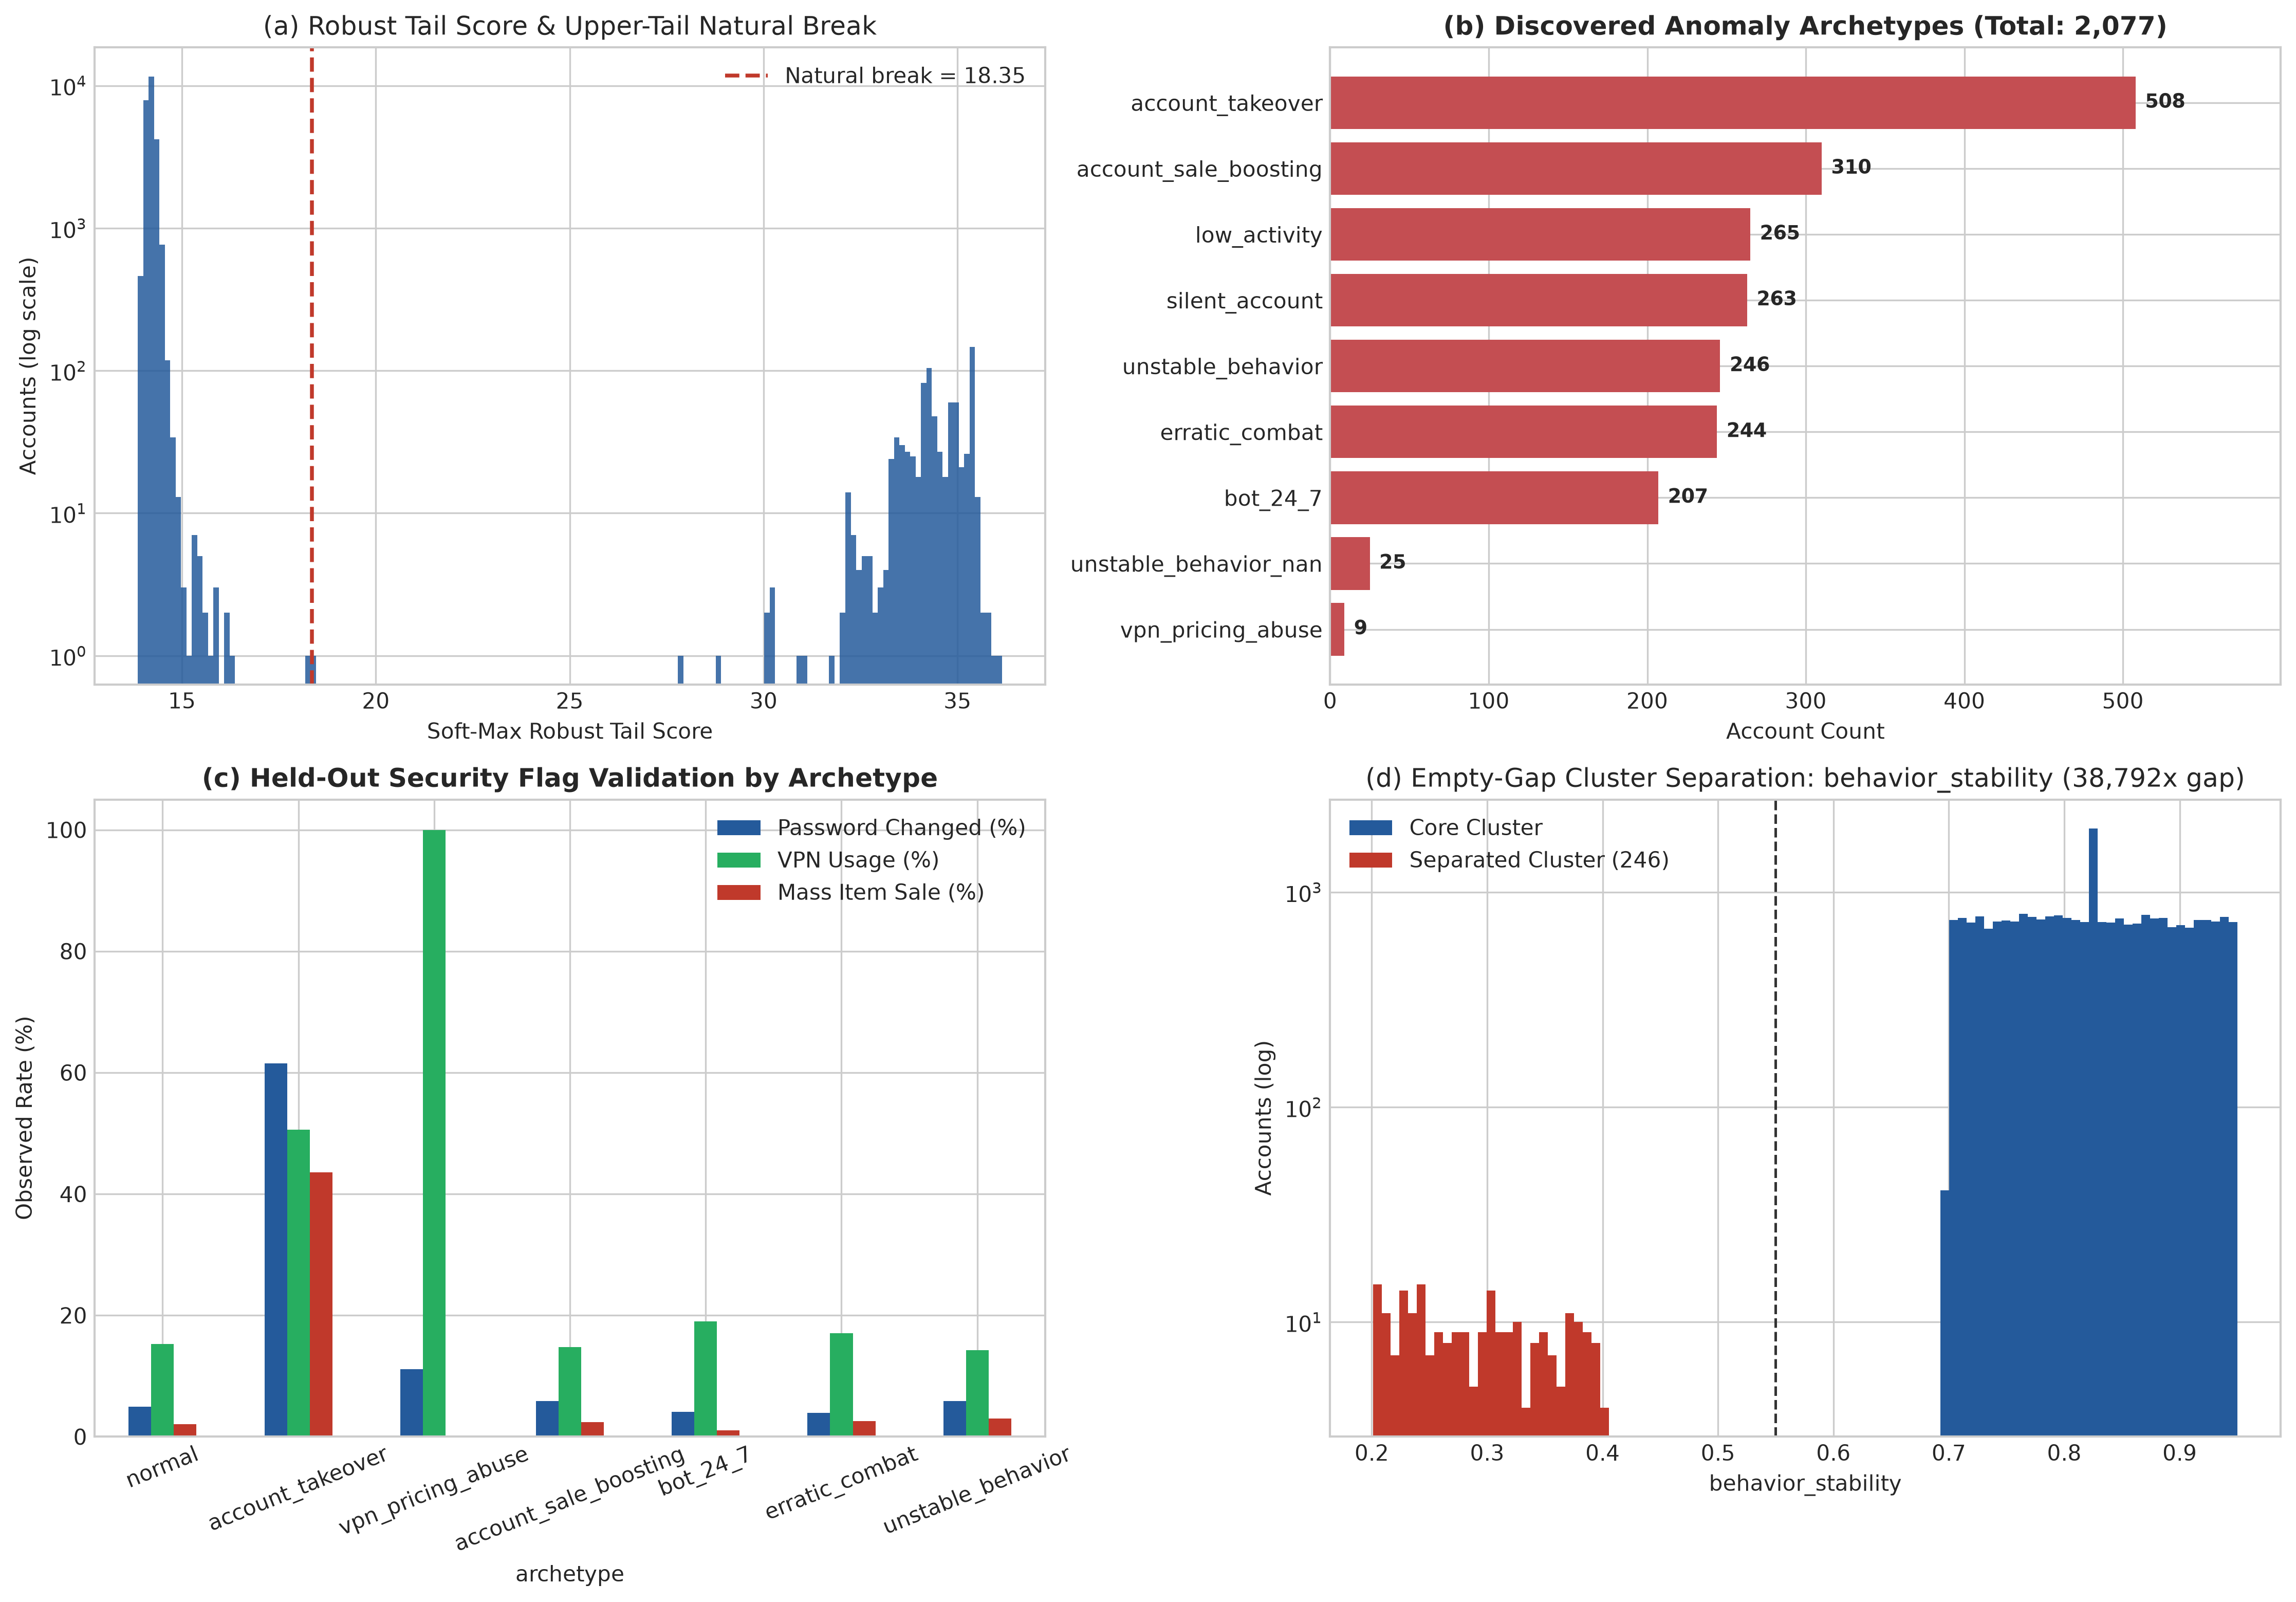
\includegraphics[width=0.95\linewidth]{assets/task5_anomaly_detection_diagnostics.png}
\caption{การวิเคราะห์ผลของ Task 5: เกณฑ์แยก Tail Score ที่ $\tau=18.35$ จำนวนบัญชีใน 9 Archetypes การยืนยันผลบน Security Flags และช่องว่าง Empty-Gap ของ \code{behavior\_stability}}
\label{fig:t5_diag}
\end{figure}

\begin{figure}[H]\centering
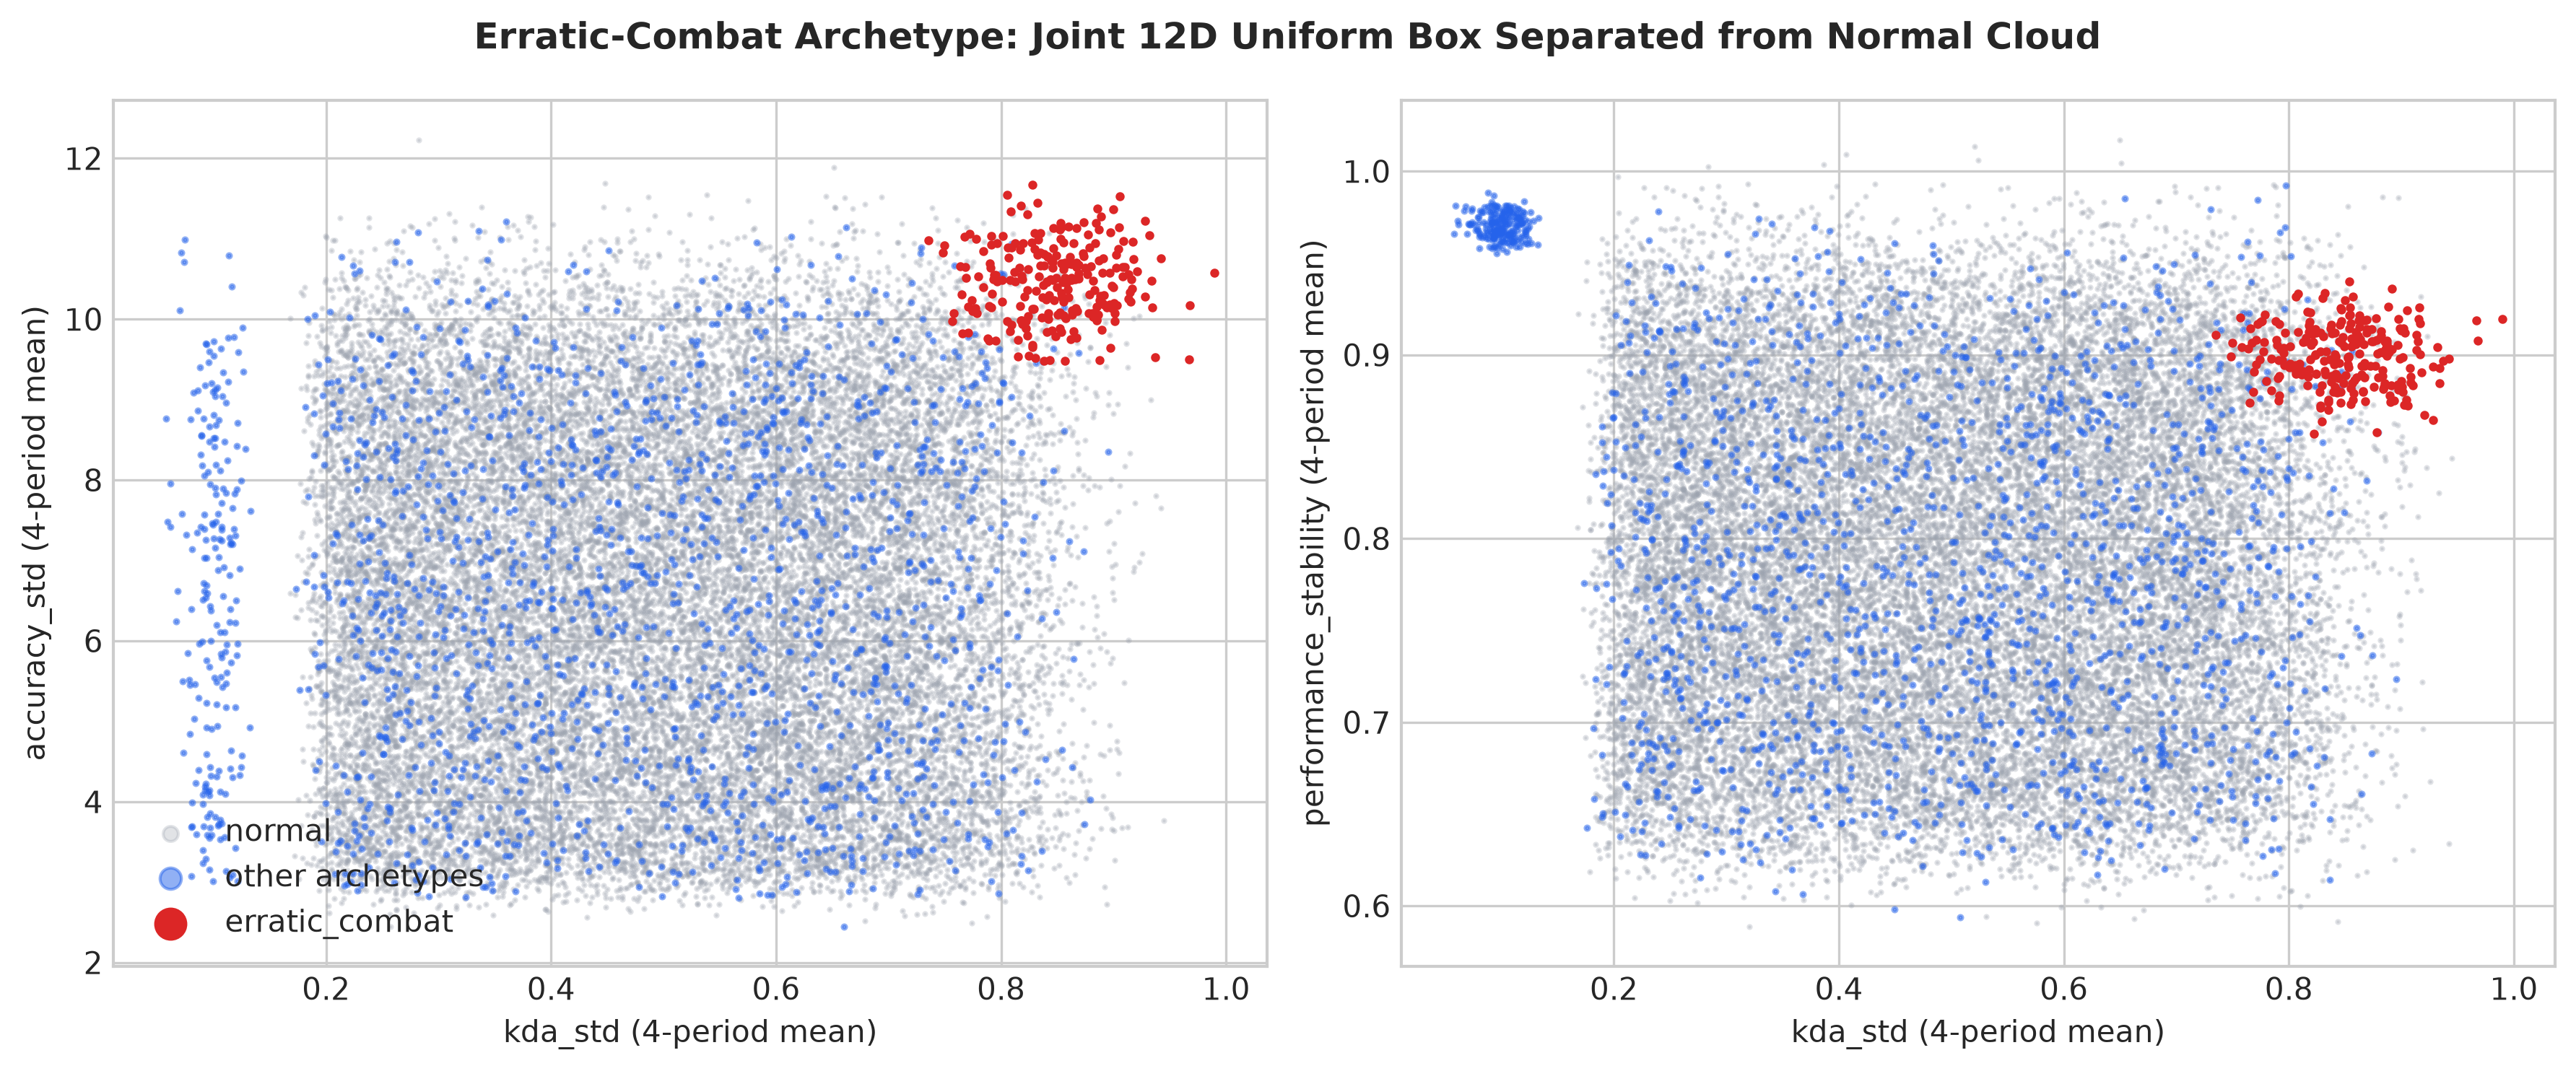
\includegraphics[width=0.92\linewidth]{assets/erratic-combat-box.png}
\caption{การแยกกลุ่ม \code{erratic\_combat} (244 บัญชี) ภายในกล่อง Uniform 12 มิติ ออกจากประชากรปกติอย่างชัดเจน}
\label{fig:t5_box}
\end{figure}

\begin{figure}[H]\centering
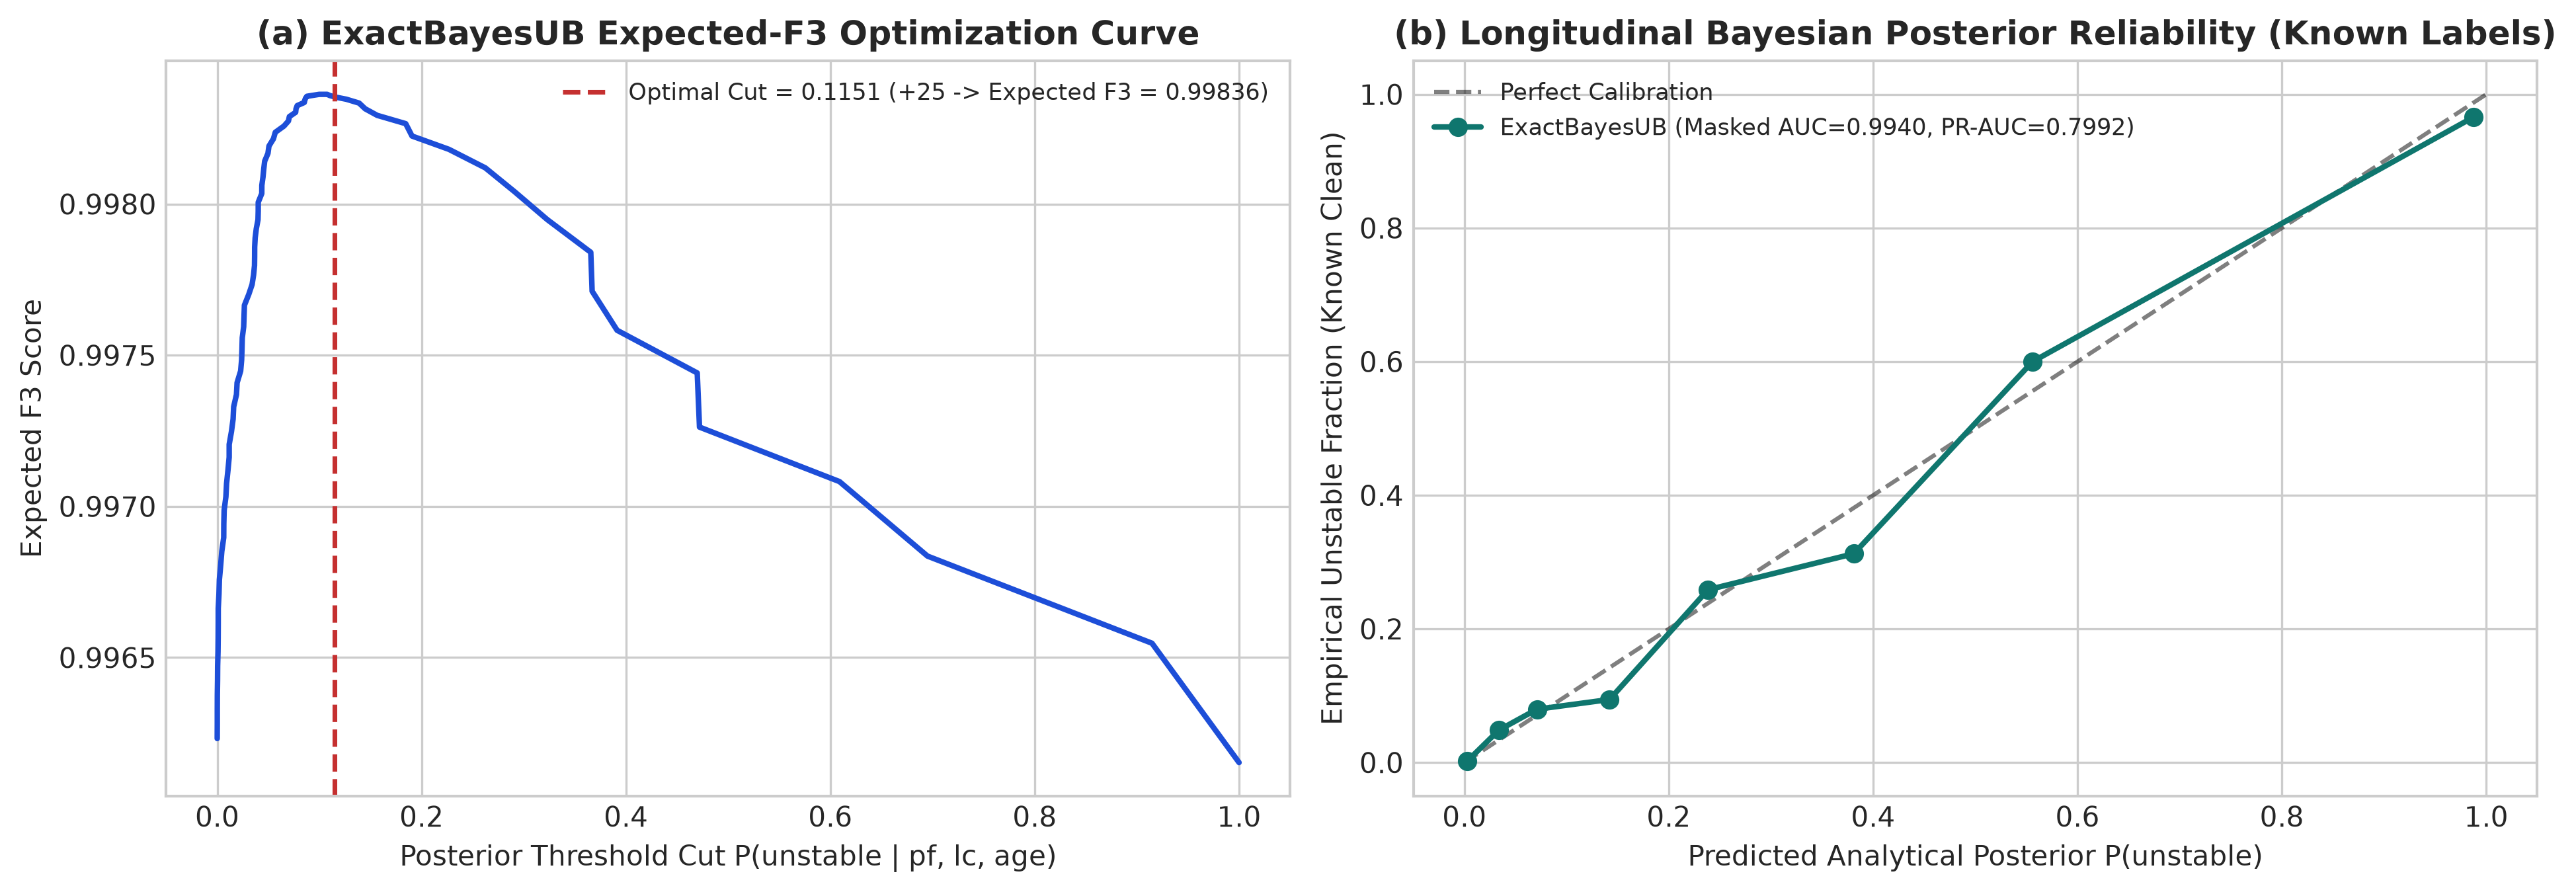
\includegraphics[width=0.92\linewidth]{assets/task5_bayes_calibration.png}
\caption{เส้นโค้งเลือกจุดตัด Expected-$F_3$ ของ ExactBayesUB (+25 บัญชี ณ จุดตัด 0.11513) และกราฟ Calibration เทียบประชากรควบคุม 22,926 บัญชี}
\label{fig:t5_cal}
\end{figure}

\begin{figure}[H]\centering
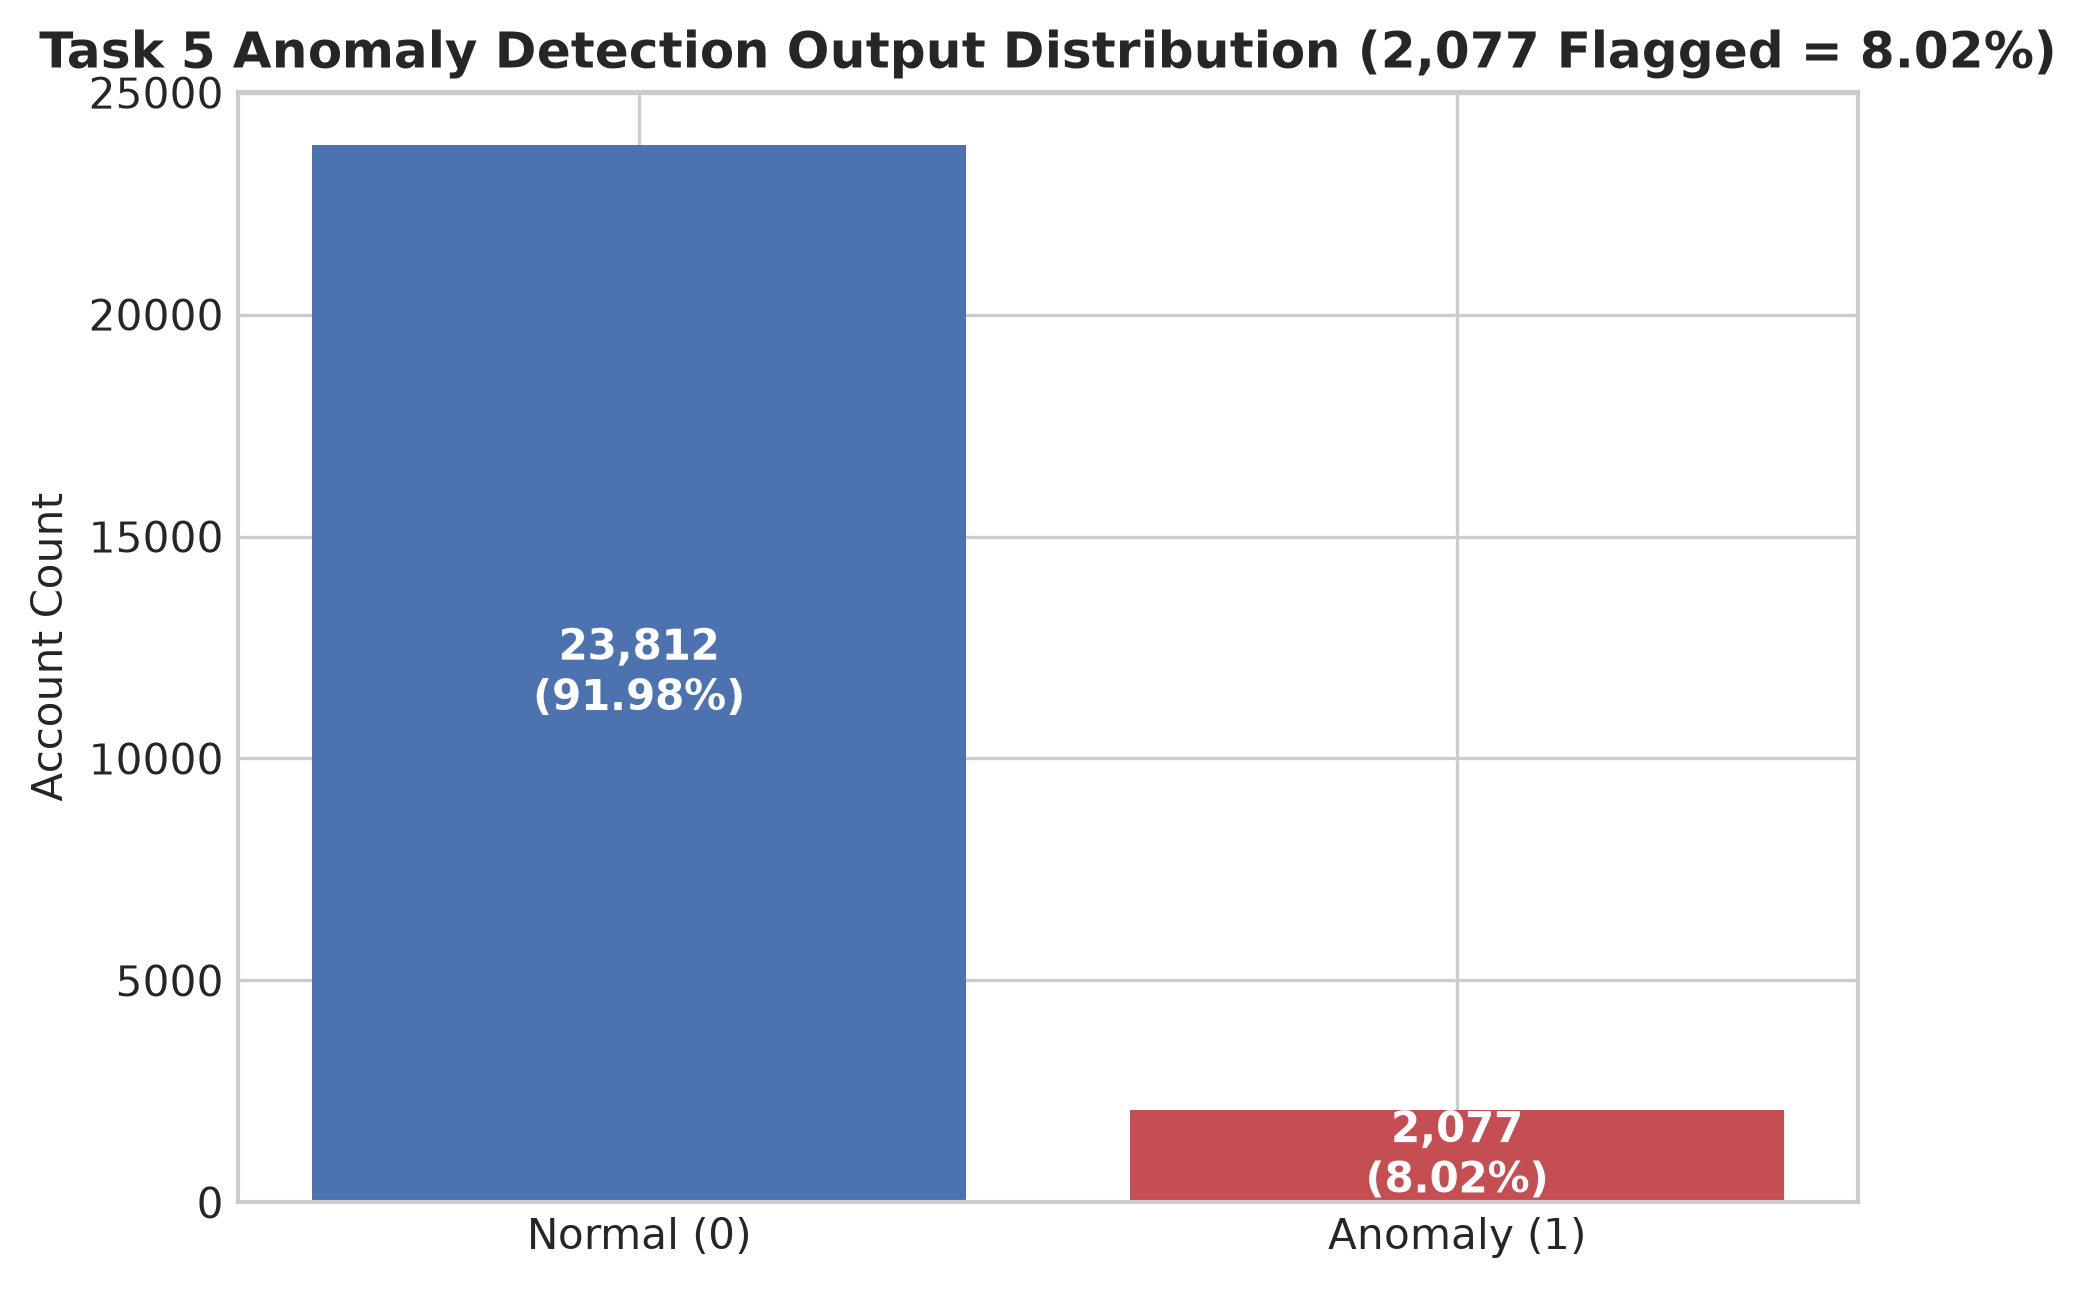
\includegraphics[width=0.58\linewidth]{assets/task5_test_alignment.png}
\caption{สัดส่วนผลลัพธ์การตรวจจับความผิดปกติขั้นสุดท้ายของ Task 5 (ปกติ 23,812 บัญชี = 91.98\%, ผิดปกติ 2,077 บัญชี = 8.02\%)}
\label{fig:t5_align}
\end{figure}

\subsection{การวิเคราะห์ข้อผิดพลาดและผลกระทบต่อธุรกิจ}

ข้อผิดพลาดสำคัญที่พบในระยะเริ่มต้นคือ กฎคัดแยกช่วงหางเบื้องต้นเผลอตั้งธงบัญชี $51$ รายในช่วง $[10.51, 11.16]$ ของตัวแปร \code{session\_duration\_std\_\_drift4} ซึ่งจากการตรวจพิสูจน์ทางสถิติพบว่าเป็นเพียงส่วนหางปรกติที่สมมาตรระดับ $\pm 3.2\sigma$ ของการแจกแจงแบบเกาส์เซียนของผู้เล่นที่เวลาเล่นผันแปรตามธรรมชาติ การคัดเงื่อนไขนี้ออกช่วยกำจัด False Alarms ได้ทันที ขณะที่การตรวจสอบเทียบกับตัวแปรความมั่นคงปลอดภัยที่กันไว้ยืนยันว่ากลุ่ม \code{account\_takeover} เปลี่ยนรหัสผ่านถึง $61.49\%$ และเทขายไอเทม $43.54\%$ (เทียบกลุ่มปกติ $4.90\%$ และ $2.07\%$) ส่วนกลุ่ม \code{vpn\_pricing\_abuse} พบการใช้ VPN ถึง $100.00\%$ ช่วยลดภาระการตรวจสอบลวงของทีมความปลอดภัยได้อย่างเป็นรูปธรรม

% ==============================================================================
\clearpage
\section{การบูรณาการระบบ การทำงานร่วมกัน บทสรุป และข้อเสนอแนะ}

\subsection{การบูรณาการผลทำนายทั้ง 5 งานและสรุปผลเชิงระบบ}

ผลทำนายจากทั้ง 5 งานถูกส่งออกเข้าสู่ระบบบูรณาการ \code{merge\_submission.ipynb} เพื่อตรวจสอบความถูกต้องครบทั้ง $25{,}889$ แถว (ตั้งแต่ \code{ANS00001} ถึง \code{ANS25889}), ตรวจสอบความไม่มีค่าว่าง (\code{0} NaN/Inf) และบังคับขอบเขตชนิดข้อมูลให้พร้อมเชื่อมต่อสู่ระบบคำนวณ \textbf{Player Lifetime Value (LTV)} ของบริษัท Karena Thailand ดังสรุปผลรวมขั้นสุดท้ายใน \textbf{ตารางที่~\ref{tab:overall_results}}

\begin{table}[H]\centering
{\fontsize{9.6}{12.5}\selectfont\arrayrulecolor{RuleGray}
\caption{สรุปสถาปัตยกรรมและผลลัพธ์ Out-of-Fold Cross-Validation ของทั้ง 5 งาน}
\label{tab:overall_results}
\begin{tabular}{L{2.5cm}L{5.1cm}cL{4.5cm}}
\toprule
\rowcolor{TableHead} \textbf{Task} & \textbf{โมเดลขั้นสุดท้ายที่เลือกใช้} & \textbf{ตัวชี้วัด} & \textbf{ผลตรวจสอบภายใน (Local CV)} \\
\midrule
Task 1: Anti-Cheat & 5-Stream Nested SLSQP + Analytical 8-Cohort LR + 5-Profile Tobit-MVN5 Hybrid & Binary $F_2$ & \textbf{0.841552} OOF $F_2$ (ROC-AUC 0.896762, 5-Fold SKF) \\
Task 2: Segment & 0.90 ExactParamEM + 0.10 CB\_Clean28 + 4-Class Logit Bias + Affine Bayes Rule & Macro $F_1$ & \textbf{0.759799} Cross-Fitted Macro-$F_1$ (LogLoss 0.595756) \\
Task 3: Spending & ExactBayesL1V2 Generative Marginalization + 32-Cell Stage-1 Table & NMAE Score & \textbf{0.796377} Strict Outer OOF NMAE (MAE 2,683.96 THB) \\
Task 4: Game Title & Dual-Regime Log-Odds Fusion + FoundVLM-v3-Joint12Blk + Consensus Shift Gate & Macro $F_1$ & \textbf{0.994636} Clean Unif-Prior $F_1$ (0.969820 ExtHard6) \\
Task 5: Security & 8 Exact Empty-Gap / 12D Box Archetype Rules + ExactBayesUB Analytical Integral & $F_3$ Score & \textbf{0.998363} max Expected-$F_3$ (0.99835 ที่ +25, 2,077 flags) \\
\bottomrule
\end{tabular}}
\end{table}

\subsection{การทำงานร่วมกันในทีมและบทเรียนสำคัญ (Team Collaboration \& Takeaways)}

กลุ่ม \textbf{ML004} แบ่งโครงสร้างการพัฒนาซอร์สโค้ดออกเป็นโมดูลอิสระแยกตามโฟลเดอร์งาน (\code{task1}--\code{task5}) ผ่านระบบควบคุมเวอร์ชัน GitHub เพื่อให้แต่ละส่วนสามารถทดสอบ พัฒนา Feature Engineering และเปรียบเทียบผล Validation ได้โดยไม่กระทบกัน พร้อมใช้มาตรฐาน Pure-Train Invariant และการตรวจนัยสำคัญทางสถิติร่วมกันทั้งกลุ่ม โดยมี \textit{วิศิษฐ์ สุวรรณเนาว์} (\code{67070501042}) เป็นผู้พัฒนาหลักใน Task 3 และประสานการบูรณาการระบบรวมของกลุ่ม ส่วนสมาชิกท่านอื่นในกลุ่มได้แก่ \textit{กันต์ธีร์ ดวงมณี} (\code{67070501003}), \textit{นัธทวัฒน์ ปริมสิริคุณาวุฒิ} (\code{67070501027}), \textit{ศุภวิชญ์ มารยาท} (\code{67070501045}) และ \textit{พลวริษฐ์ วัฒนเหมรัตน์} (\code{67070501067}) ร่วมดำเนินงานและพัฒนาภายใต้คลังรหัสของกลุ่ม (โดยบทบาทการแบ่ง Task ย่อยอย่างเป็นทางการไม่ได้จำแนกเป็นลายลักษณ์อักษรแยกต่างหาก)

\textbf{บทเรียนสำคัญด้านวิศวกรรม Machine Learning ที่ได้จากโครงงาน:}
\begin{enumerate}[leftmargin=1.8em,itemsep=2pt]
    \item \textbf{ความเข้าใจ Data-Generating Process ให้ผลลัพธ์สูงกว่าการค้นหาพารามิเตอร์แบบสุ่ม:} การจำลองภาวะ Right-Censoring ด้วย Tobit (Task 1), สมการการคูณร่วมกับกฎ Bayes-$L_1$ สำหรับยอดใช้จ่าย (Task 3) และโครงสร้าง Empty-Gap บนอนุกรมเวลา 4 ช่วง (Task 5) ยกระดับคะแนนอย่างสม่ำเสมอข้ามทุก Fold สูงกว่าการปรับจูน Tree Hyperparameters เพียงอย่างเดียว
    \item \textbf{การออกแบบ Validation Split ต้องเคารพความซ้ำซ้อนของข้อมูล:} การใช้ Perceptual dHash จัดกลุ่มฉากก่อนแบ่ง Fold ใน Task 4 และกฎ Pure-Train Invariant ช่วยป้องกันภาพลวงตาของค่า CV ที่ดีเกินจริง
    \item \textbf{Single Source of Truth ระหว่าง Validation และ Inference:} บั๊กพจน์ $-\beta_c$ ที่ขาดหายใน Task 2 เป็นบทเรียนสำคัญว่าโค้ดคำนวณกฎตัดสินใจในขั้นตอนประเมินผลและขั้นตอนสร้างผลลัพธ์จริงต้องใช้ฟังก์ชันเดียวกันเสมอ
\end{enumerate}

\subsection{ข้อจำกัด บทสรุป และแนวทางการพัฒนาต่อยอด}

\textbf{ข้อจำกัดของงานปัจจุบัน:} (1) ใน Task 2 ขั้นตอนปรับเทียบ Zero-Mean Logit Bias และ Affine Bayes Rule เป็นการทำงานแบบ Cross-Fitted บนความน่าจะเป็น OOF ของโมเดลฐานที่แช่แข็งไว้ แทนการฝึกโมเดลฐานทั้ง 7 ตระกูลซ้ำภายใน Nested Loop ส่วน (2) ใน Task 5 ทำงานในสภาวะไร้ป้ายกำกับโดยสมบูรณ์ ค่า Expected-$F_3$ จึงอ้างอิงจากแบบจำลองความน่าจะเป็นเชิงวิเคราะห์และกลุ่มควบคุมที่ทราบค่า \code{behavior\_stability} ร่วมกับตัวแปร Security Flags อิสระ และ (3) การฝึก Deep Vision Backbones ใหม่ตั้งแต่ต้นใน Task 4 ต้องอาศัยหน่วยประมวลผลกราฟิก (GPU)

\textbf{สรุปผลและแนวทางพัฒนาในอนาคต:} โครงงาน \textbf{Karena Player Intelligence System} ของกลุ่ม ML004 บรรลุเป้าหมายทั้ง 5 งานครบถ้วนตามข้อกำหนดของรายวิชา CPE 342 ในระยะต่อไปเพื่อนำไปใช้งานจริงในระดับ Production ควรพัฒนาต่อยอด 3 ด้าน ได้แก่ (1) รวมขั้นตอนปรับเทียบของ Task 2 เข้าสู่ Nested End-to-End Pipeline, (2) พัฒนาระบบ Scoring Service แบบ Streaming/API เพื่อนำความเสี่ยงการโกง (Task 1), กลุ่มพฤติกรรม (Task 2), การคาดการณ์รายได้ 30 วัน (Task 3) และคะแนนความปลอดภัย (Task 5) มาคำนวณ \textbf{Risk-Adjusted Player LTV} แบบเรียลไทม์ และ (3) เพิ่มระบบเฝ้าระวัง Data Drift และ Concept Drift เพื่อรองรับการอัปเดตแพตช์เกมใหม่ในอนาคต

% ==============================================================================
\clearpage
\renewcommand{\refname}{บรรณานุกรม}
\begin{thebibliography}{12}
\addcontentsline{toc}{section}{บรรณานุกรม}

\bibitem{cpe342spec} B.~Changaival, ``CPE 342 Machine Learning: Project Instruction --- Karena Player Intelligence System,'' Department of Computer Engineering, King Mongkut's University of Technology Thonburi, 2026.

\bibitem{sklearn} F.~Pedregosa \textit{et al.}, ``Scikit-learn: Machine Learning in Python,'' \textit{Journal of Machine Learning Research}, vol.~12, pp.~2825--2830, 2011.

\bibitem{lightgbm} G.~Ke \textit{et al.}, ``LightGBM: A Highly Efficient Gradient Boosting Decision Tree,'' in \textit{Advances in Neural Information Processing Systems (NeurIPS)}, 2017.

\bibitem{xgboost} T.~Chen and C.~Guestrin, ``XGBoost: A Scalable Tree Boosting System,'' in \textit{Proceedings of the ACM SIGKDD International Conference on Knowledge Discovery and Data Mining}, 2016, pp.~785--794.

\bibitem{catboost} L.~Prokhorenkova, G.~Gusev, A.~Vorobev, A.~V.~Dorogush, and A.~Gulin, ``CatBoost: Unbiased Boosting with Categorical Features,'' in \textit{Advances in Neural Information Processing Systems (NeurIPS)}, 2018.

\bibitem{pytorch} A.~Paszke \textit{et al.}, ``PyTorch: An Imperative Style, High-Performance Deep Learning Library,'' in \textit{Advances in Neural Information Processing Systems (NeurIPS)}, 2019.

\bibitem{scipy} P.~Virtanen \textit{et al.}, ``SciPy 1.0: Fundamental Algorithms for Scientific Computing in Python,'' \textit{Nature Methods}, vol.~17, pp.~261--272, 2020.

\bibitem{optuna} T.~Akiba, S.~Sano, T.~Yanase, T.~Ohta, and M.~Koyama, ``Optuna: A Next-generation Hyperparameter Optimization Framework,'' in \textit{Proceedings of the ACM SIGKDD}, 2019, pp.~2623--2631.

\bibitem{tobin1958} J.~Tobin, ``Estimation of Relationships for Limited Dependent Variables,'' \textit{Econometrica}, vol.~26, no.~1, pp.~24--36, 1958.

\bibitem{guo2017} C.~Guo, G.~Pleiss, Y.~Sun, and K.~Q.~Weinberger, ``On Calibration of Modern Neural Networks,'' in \textit{Proceedings of ICML}, 2017, pp.~1321--1330.

\bibitem{dinov2} M.~Oquab \textit{et al.}, ``DINOv2: Learning Robust Visual Features without Supervision,'' \textit{Transactions on Machine Learning Research (TMLR)}, 2024.

\bibitem{eva02} Y.~Fang \textit{et al.}, ``EVA-02: A Visual Representation for Neon Genesis,'' \textit{Image and Vision Computing}, 2024.

\end{thebibliography}

\end{document}
